\chapter{Revisão bibliográfica}

\section{Aprendizado de Máquina }

\subsection{Modelo McCulloch-Pitts}
Para que seja possível iniciar uma discussão acerca de redes neurais artificiais, é necessário voltar a atenção para o primeiro modelo de neurônio biológico proposto por McCulloch e Pitts em 1943. Este é o modelo mais clássico de neurônio em RNA (redes neurais artificiais), proposto em um trabalho intitulado ``Um cálculo lógico das ideias intrínsecas da atividade neural'' \cite{zuben_attux}.

Em um neurônio biológico, as sinapses possuem canais que permitem a entrada e saída de íons de modo que torna o neurônio capaz de receber sinais de entrada através da mesma. Dependendo da intensidade resultante destes sinais de entrada, isto é, se a intensidade resultante for superior a um determinado limiar, o neurônio libera neurotransmissores na sinapse, o que por sua vez corresponde à emissão de um sinal de saída.

McCulloch e Pitts então empreenderam a primeira tentativa de entender a atividade neural a partir de unidades elementares  da computação, construindo um modelo baseado em simplificações do que se sabia na época sobre o neurônio biológico. Seu modelo é baseado principalmente nas seguintes premissas \cite{zuben_attux},\cite{jacson}:

\begin{itemize}
\item O neurônio tem apenas dois estados: ativo ($1$) ou inativo ($0$);
\item Uma certa quantidade fixa de sinapses deve ser excitada de forma a excitar o neurônio;
\item A atividade de uma sinapse inibitória bloqueia completamente a atividade do neurônio.
\end{itemize}

Matematicamente então, o neurônio de McCulloch Pitts, a cada iteração:
\begin{itemize}
\item Soma as entradas com peso unitário $\sum_{j}x_{j}$;
\item Se esse valor ultrapassar um limiar $\theta$, e a entrada inibitória $x_i$ não estiver ativa ($0$), o neurônio é ativado ($1$);
\item Se não, o neurônio permanece inativo ($0$).
\end{itemize}
Isto é:
\begin{equation}f\left(x_{1},\dots,x_{N}\right)=\left\{ \begin{array}{ccccc}
1 & se & \sum_{j=1}^{N}x_{j}>\theta & e & x_{i}=0\\
0 & se & \sum_{j=1}^{N}x_{j}\leq\theta & ou & x_{i}=1
\end{array}\right. . \end{equation}

Evidentemente, esse modelo apresenta algumas limitações, dentre elas pode-se destacar que o mesmo não é capaz de aprender a partir dos dados disponíveis nem diferenciar a importância das entradas e, por fim, a entrada inibitória ainda pode ser uma limitação inconveniente.

\subsection{Modelo de Rosenblatt}

Nos anos de 1950 e 1960, Frank Rosenblatt, inspirado pelo trabalho de Warren McCulloch e Waltper Pitts, desenvolve seu próprio modelo, conhecido também como perceptron \cite{nielsen2015neural}. Rossenblatt propôs modificações simples para o cálculo da saída, dentre as quais pode-se destacar a introdução de pesos diferentes para cada entrada e a remoção da entrada inibitória.

Utilizando os pesos, foi capaz de expressar as diferentes importâncias que cada entrada poderia possuir. Então sendo o peso $w_j$ correspondente à entrada $x_j$ e mantendo a notação do limiar $\theta$, a saída do neurônio $f$ é dada por:
\begin{equation}f\left(x_{1},\dots,x_{N}\right)=\left\{ \begin{array}{ccc}
1 & se & \sum_{j=1}^{N}w_{j}x_{j}>\theta\\
0 & se & \sum_{j=1}^{N}w_{j}x_{j}\leq\theta
\end{array}\right. . \end{equation}
Onde foi pequena alteração da notação, o limiar foi passado para outro lado da igualdade, onde recebe o nome de viés ($b=-\theta$) . Isto é:
\begin{equation}
f\left(x_{1},\dots,x_{N}\right)=\left\{ \begin{array}{ccc}
1 & se & \sum_{j=1}^{N}w_{j}x_{j}+b>0\\
0 & se & \sum_{j=1}^{N}w_{j}x_{j}+b\leq0
\end{array}\right.\rightarrow f\left(x_{1},\dots,x_{N}\right)=\left\{ \begin{array}{ccc}
1 & se & \sum_{j=1}^{N}w_{j}x_{j}>\theta\\
0 & se & \sum_{j=1}^{N}w_{j}x_{j}\leq\theta
\end{array}\right.
\end{equation}
o somatório do produto entre pesos e entradas pode ser escrito como um produto interno, utilizando a notação da Mecânica Quântica:
\begin{equation}f=\left\{ \begin{array}{ccc}
1 & se & \left\langle w|x\right\rangle +b>0\\
0 & se & \left\langle w|x\right\rangle +b\geq0
\end{array}\right. . \end{equation}
Onde:
\begin{equation}\left\langle w|x\right\rangle =\overrightarrow{w}\cdot\overrightarrow{x}=\left[\begin{array}{cccc}
w_{1} & w_{2} & \cdots & w_{N}\end{array}\right]^{T}\left[\begin{array}{c}
x_{1}\\
x_{2}\\
\vdots\\
x_{N}
\end{array}\right]=\sum_{j=1}^{N}w_{j}x_{j} .\end{equation}
Pode-se  perceber que o viés é equivalente a uma entrada $x_b=b$ com um peso $w_b=1$. Um exemplo prático da usabilidade de perceptrons é a possibilidade de construção da porta lógica NAND. Considerando um perceptron com um viés de $b=3$  e duas entradas com pesos iguais $w_1=w_2=-2$, e passando a denotar o somatório como função ativação $z\left(x_{1},x_{2}\right)$ tem-se:
\begin{equation}z=-2x_{1}-2x_{2}+3.\end{equation}
A partir da função ativação é possível construir a seguinte tabela de entradas e saídas:
\begin{center}
\begin{tabular}{|l|l|l|l|}
\hline
$x_1$ & $x_2$ & $z$ & $f$ \\ \hline
0     & 0     & 3   & 1                                             \\ \hline
1     & 0     & 1   & 1                                             \\ \hline
0     & 1     & 1   & 1                                             \\ \hline
1     & 1     & -1  & 0                                             \\ \hline
\end{tabular}
\end{center}
Esta tabela é idêntica a tabela verdade da porta NAND. A NAND é uma porta universal para a computação clássica. Deste modo, o perceptron também é universal para a computação clássica, e através de uma rede de perceptrons é possível computar qualquer função lógica \cite{nielsen2015neural}.

Porém, a maior novidade que surge em comparação ao modelo anterior, é que uma vez que a entrada inibitória pode ser simulada por entradas simples \cite{rojas}, a remoção dela junto com as outras modificações propostas por Rosenblatt tornou seu modelo mais flexível, e concedeu a capacidade ao perceptron de ter seus pesos e viés atualizados através de um algoritmo de aprendizado. Isto é, sem uma intervenção direta pelo programador. O algoritmo de aprendizagem nos permite resolver problemas que são extremamente difíceis de se propor um modelo diretamente, um exemplo que podemos citar são problemas de classificação de imagens.

\subsubsection{Regra de aprendizado}

Rosenblatt provou que a regra de aprendizado proposta em seu trabalho sempre converge para os pesos corretos para resolver o problema em questão, se estes pesos existirem. A regra de aprendizado também é conhecida como algoritmo de aprendizado, ou algoritmo de treinamento \cite{NND}. O algoritmo do perceptron é do tipo  aprendizado supervisionado. Isto significa que é fornecido um conjunto de exemplos (dados de treinamento) do comportamento apropriado da rede:
\begin{equation}\left\{ \left|x_{1}\right\rangle ,t_{1}\right\} ,\left\{ \left|x_{2}\right\rangle ,t_{2}\right\} ,\dots,\left\{ \left|x_{N}\right\rangle ,t_{N}\right\} . \end{equation}
Onde $t_j$ é o saída desejada correspondente à entrada $\left|x_{j}\right\rangle $. Então a regra de aprendizado é usada para ajustar os pesos e o viés do neurônio de modo  a mover as saídas do mesmo para mais próximo às saídas desejadas. Um conceito importante é a fronteira de decisão. Esta é definida para quando a função de ativação é igual a zero, isto é:
\begin{equation}z=\left\langle w|x\right\rangle +b=0.\end{equation}A fronteira de decisão é um hiperplano (um sub-espaço de dimensão $N-1$ em um espaço de dimensão $N$) no espaço de entrada. Para ficar mais concreto, como exemplo pode-se restringir a análise à duas entradas, então se o espaço de entrada tem 2 dimensões $\left(x_{1},x_{2}\right)=\left(x,y\right)$, logo o hiperplano é uma reta (1 dimensão)  em que a saída é $0$ de um lado e $1$ do outro. Especificamente:
\begin{equation}
\begin{split}
x_{1}w_{1}+w_{2}x_{2}+b=0, \\
x_{2}=-\frac{w_{1}}{w_{2}}x_{1}-\frac{b}{w_{2}}.
 \end{split}
\end{equation}
 Isto é uma equação da reta do tipo $y=ax+b$ onde $a=-\frac{w_{1}}{w_{2}}$ e $b=-\frac{b}{w_{2}}$. Sendo $a$  a inclinação da reta, um vetor perpendicular a fronteira de decisão deve ter a inclinação $\left(-\frac{1}{a}\right)=\frac{w_{2}}{w_{1}}$. Portanto o vetor peso $\left|w\right\rangle $ é perpendicular a reta formada pela fronteira de decisão.  Desta maneira, este perceptron é capaz de classificar corretamente um conjunto de dados de duas dimensões no qual as duas classes podem ser separadas por uma reta. O algoritmo de aprendizado é responsável por ajustar a inclinação (através dos pesos) e a distância da origem (pelo viés) desta reta.

Desta maneira, é possível compreender as regras de aprendizado do perceptron para atualização dos pesos em 3 regras:
 
 \begin{itemize}
	 \item Se foi classificado corretamente, não realizamos nenhuma alteração;
 \item Se era para ser classificado como $t=1$, e foi classificado errado $f=0$, soma-se o vetor de entrada: $\left|w\right\rangle '=\left|w\right\rangle '+\left|x\right\rangle $;
 \item Se era para ser classificado como $t=0$, e foi classificado errado $f=1$, subtrai o vetor de entrada: $\left|w\right\rangle '=\left|w\right\rangle '-\left|x\right\rangle $.
 \end{itemize}
 
 Dessa maneira, aproxima-se o vetor peso $\left|w\right\rangle$ do vetor de entrada $\left|x\right\rangle $ quando a classificação deveria ser $t=1$ e o foi classificado errado, e afasta-se quando a classificação correta é $t=0$ mas foi classificado incorretamente.  Essas três regras ainda podem ser unificadas ao se notar que o sinal da operação com o vetor $\left|x\right\rangle $  pode ser descrito pela diferença $e=\left(t-f\right)$, que nada mais é do que uma medida simples do erro. Dessa maneira, de forma unificada pode-se escrever: \begin{equation}\left|w\right\rangle '=\left|w\right\rangle '+e\left|x\right\rangle . \end{equation}
E lembrando que o viés pode ser descrito como um peso para uma entrada em que a entrada é $x_j=1$, de maneira análoga:
\begin{equation}b'=b+e . \end{equation}
A fim de aumentar o controle sobre a aprendizagem, pode-se considerar ainda uma taxa de aprendizado $\eta$ :
\begin{equation}
\begin{split}
\left|w\right\rangle ' & =\left|w\right\rangle '+ e \eta \left|x\right\rangle, \\
b' & =b+\eta e.
\end{split}
\end{equation}
Perceptrons ainda são naturalmente limitados, essas limitações foram demonstradas em um livro chamado Perceptrons por Marvin Minsky e Seymour Papert. A fronteira de decisão do perceptron é linear, logo um perceptron pode ser usado para classificar problemas que podem ser descritos de maneira linearmente separável, porém infelizmente muitos problemas não são linearmente separáveis, como a porta lógica XOR \cite{NND}.


\subsection{Modelo Sigmoide}

Outra limitação mais evidente do modelo do perceptron se encontra nos valores de saída que são binários. Além disso a regra de aprendizado foi desenhada para atualizar os valores de cada perceptron individualmente, então para a construção de uma rede neural em que se utiliza a saída de um perceptron ($p_{11}$) como entrada de outro perceptron ($p_{12}$), seria necessário saber qual é o valor intermediário esperado  (a saída de $p_{11}$, que serve de entrada para $p_{12}$). Deste modo, para a construção de uma rede neural mais complexa, é necessário também um modelo genérico mais complexo.

Sigmoide é um tipo de neurônio artificial similar aos perceptrons, porém modificado para que pequenas variações nos pesos e viés causem apenas uma pequena variação na saída, uma vez que agora a saída é um valor contínuo. É por isso que sigmoides são os principais modelos de neurônios e junto com o algoritmo de aprendizado do gradiente descendente permitem a construção de redes mais complexas.

Para atingir esse objetivo, o neurônio sigmoide aceita entradas e saída entre $0$ e $1$, ou seja, não trabalha mais apenas com valores binários na saída. A função ativação clássica de um sigmoide é:
\begin{equation}f\left(x_{1},\dots,x_{N}\right)\equiv\frac{1}{1+e^{-\left(\left\langle w|x\right\rangle -b\right)}}. \end{equation}
Pode-se conferir que para casos extremos em que $g=\left\langle w|x\right\rangle -b\rightarrow\infty$ e $g= \left\langle w|x\right\rangle -b\rightarrow -\infty,$  a função vale respectivamente:
\begin{equation}
\begin{split}
\lim_{g\rightarrow\infty}f & =\lim_{g\rightarrow \infty}\frac{1}{1+e^{-g}}=1, \\
\lim_{g\rightarrow-\infty}f & =\lim_{g\rightarrow-\infty}\frac{1}{1+e^{-g}}=0.
\end{split} 
\end{equation}
Desta maneira, a função sigmoide mantém a saída entre os valores $0$ e $1$, porém não mais de forma binária, mas de maneira suave.

\subsubsection{Gradiente descendente}

A mudança na função de ativação do neurônio sigmoide permite que seja utilizado um novo algoritmo de aprendizado, mais complexo, mas que também permite a construção de redes mais complexas. Como a regra de aprendizado visa aproximar os pesos e viés de maneira que o resultado da rede se aproxime do resultado esperado, é interessante que seja possível quantificar o erro da rede ao classificar um conjunto de dados de treinamento. Assim, pode-se concentrar em minimizar esse valor.

Com esta finalidade define-se uma função custo, isto é, uma função que serve exatamente para quantificar  o erro. Considerando que a rede pode apresentar mais de uma saída, pode-se escrever o vetor de saídas desejadas para um determinado vetor de entrada $\left|x_j\right\rangle $ como $\left|d_j\right\rangle $ . De forma mais explícita, para $M$ saídas possíveis temos  $ \left|d_{j}\right\rangle =\left[\begin{array}{cccc}
d_{j1} & d_{j2} & \dots & d_{jM}\end{array}\right]^{T} $. Então o elemento $d_{ji}$  corresponde à saída desejada pelo neurônio $i$ para o vetor de entrada $j$. De forma análoga, pode-se escrever o vetor dos resultados obtidos pela rede como $\left|f_{j}\right\rangle $. A partir desta notação, uma típica função custo pode ser escrita, para $N$ pesos e $K$  entradas, como \cite{nielsen2015neural}:
\begin{equation}C\left(w_{1},\dots,w_{N},b\right)=\frac{1}{2K}\sum_{j=1}^{K}\left\Vert \left|d_{j}\right\rangle -\left|f_{j}\right\rangle \right\Vert ^{2} . \end{equation}
Onde a norma de um vetor $\left|x\right\rangle $  é definida como $\left\Vert \left|x\right\rangle \right\Vert =\sqrt{\left\langle x|x\right\rangle }$. Quando os pesos são atualizados, a expectativa é de que ocorra uma diminuição do valor da função custo, isto é, uma variação negativa. Para tornar os cálculos mais compactos, uma alternativa é absorver o viés no vetor dos pesos como um peso $w_{N+1}=b$. 
\begin{equation}\left|w\right\rangle =\left[\begin{array}{c}
w_{1}\\
w_{2}\\
\vdots\\
w_{N}\\
b
\end{array}\right]=\left[\begin{array}{c}
w_{1}\\
w_{2}\\
\vdots\\
w_{N}\\
w_{N+1}
\end{array}\right]\qquad\left|x\right\rangle =\left[\begin{array}{c}
x_{1}\\
x_{2}\\
\vdots\\
x_{N}\\
1
\end{array}\right]=\left[\begin{array}{c}
x_{1}\\
x_{2}\\
\vdots\\
x_{N}\\
x_{N+1}
\end{array}\right] . \end{equation}
A diferencial total da função custo é dada por:
\begin{equation}
\begin{split}
dC&=\sum_{j=1}^{N+1}\frac{\partial C}{\partial w_{j}}dw_{j}, \\
\Delta C&\approx\sum_{j=1}^{N+1}\frac{\partial C}{\partial w_{j}}\Delta w_{j}.
\end{split} 
\end{equation}
Pela definição do gradiente para $N+1$ dimensões do espaço de pesos temos $\nabla_w\equiv\sum_{j=1}^{N+1}\widehat{w}_{j}\frac{\partial}{\partial w_{j}}$, e definindo um vetor de variações dos pesos como $\left|\Delta w\right\rangle =\sum_{j=1}^{N+1}\Delta w_{j}\widehat{w}_{j}$,  é possível então reescrever a variação da função custo como:
\begin{equation}\Delta C\approx\nabla_{w}C\cdot\left|\Delta w\right\rangle . \end{equation}
Supondo uma variação no vetor peso da seguinte forma: $\left|\Delta w \right\rangle =-\eta\nabla_{w}C$,  espera-se que a função custo seja minimizada. Pois a diferencial da função custo torna-se, desde que a variação proposta seja pequena o suficiente:
\begin{equation}
\begin{split}
\Delta C & \approx\nabla_{w}C\cdot\left|\Delta w\right\rangle, \\
& \approx \nabla_{w}C\cdot\left(-\eta\nabla_{w}C\right), \\
 & \approx -\eta\left\Vert \nabla_{w}C\right\Vert ^{2}.
\end{split} 
\end{equation}
Onde $\eta$  é chamada de taxa de aprendizado, análogo ao caso do perceptron. Portanto o algoritmo do gradiente descendente consiste em atualizar os pesos da seguinte forma:
\begin{equation}
\begin{split}
\left|w\right\rangle ' & =\left|w\right\rangle +\left|\Delta w\right\rangle, \\
& =\left|w\right\rangle -\eta\nabla_{w}C.
\end{split}  
\end{equation}
E o gradiente da função custo, de forma mais específica:
\begin{equation}
\begin{split}
\nabla_{w}C & =\frac{1}{2K}\sum_{j=1}^{N}\left(\nabla_{w}\left\Vert \left|d_{j}\right\rangle -\left|f_{j}\right\rangle \right\Vert ^{2}\right) \\
 & =\frac{1}{K}\sum_{j=1}^{K}\left(\left\Vert \left|d_{j}\right\rangle -\left|f_{j}\right\rangle \right\Vert \right)\left(\nabla_{w}\left\Vert \left|d_{j}\right\rangle -\left|f_{j}\right\rangle \right\Vert \right) .
 \end{split}  
 \end{equation}
Isto decorre da regra da cadeia. Vale destacar que enquanto $\left|d_{j}\right\rangle $ é um vetor de constantes, o vetor $\left|f_{j}\right\rangle $ é formado por elementos $f_{ji}$  que são obtidos através da função de ativação. O primeiro termo entre parênteses no gradiente da função custo é simplesmente a diferença entre os resultados desejados e o obtido pela rede. Como a regra de aprendizado é aplicada depois da rede classificar os dados de treinamento, isto pode ser obtido diretamente a partir dos valores resultantes, sendo assim, resta unicamente a tarefa de calcular o segundo termo, que vai depender de detalhes específicos da rede.

Apesar de envolver um cálculo mais complicado que para o caso do perceptron, este algoritmo de aprendizado possui a vantagem de que só é necessário  saber as saídas desejadas de toda a rede para aplicar a regra de aprendizado em cada um dos neurônios que compõem esta mesma rede.

\subsection{Método Kernel}

Perceptrons e sigmoides são modelos que são relativamente fáceis de implementar e otimizar, mas são classificadores lineares, isto é, são limitados a fronteiras de decisões lineares, é para lidar com essa questão que surge o método kernel. Este método tem como principal objetivo capturar padrões não-lineares nos dados mapeando-os em dimensões mais elevadas no qual exibem um padrão linear \cite{kernel2}.  Isto é feito à custas de um aumento no custo computacional necessário para realizar o treinamento. Porém, uma das vantagens que a computação quântica nos oferece em comparação à computação clássica é o aumento no poder computacional, uma vez que a quantidade de coeficientes aumenta exponencialmente com a quantidade de qubits e a natureza da mecânica quântica nos permite utilizar recursos de paralelismo. O problema que o método kernel se propõe a solucionar pode ser enunciado da seguinte forma: tendo duas classes de objetos,  para um novo  novo objeto é necessário classificá-lo em uma das classes  \cite{kernel}.

Considerando então os seguintes dados empíricos:
\begin{equation}
\left(x_{1},y_{1}\right),\dots,\left(x_{m},y_{m}\right)\in\mathcal{X}\times\left\{ \pm1\right\}  .
\end{equation}Onde:
\begin{itemize}
\item  $ \mathcal{X} $: conjunto de onde os padrões $x_{i}$ são retirados, chamado também de domínio;
\item $ x_{i}\rightarrow $ entradas, casos, instâncias, observações;
\item  $\left\{ \pm1\right\}$: conjunto onde retira-se as saídas $y_{i}$:
\item $y_{i}\rightarrow $ rótulos, alvos, saídas, observações.
\end{itemize}
 
Pode-se notar que há somente duas classes, ou seja, um padrão de reconhecimento ou classificação binária. É necessário um tipo adicional de estrutura, para generalizar os dados que não estamos vendo. Isto é, de maneira esquematizada:

\begin{enumerate}
\item Dado um novo padrão $ x\in\mathcal{X}$, queremos predizer o correspondente $y\in\left\{ \pm1\right\}$ ;
\item Fazendo isso para cada $x\in\mathcal{X}$ nos leva a estimar uma função $f : X\rightarrow\left\{ \pm1\right\}$;
\item Queremos escolher $y$ de forma que $\left(x,y\right)$ seja coerente aos exemplos de treinamento;
\item Precisamos então ter noções de similaridade em $\mathcal{X}$ e $\left\{ \pm1\right\}$.
\end{enumerate}

A similaridade da saída é obtida de forma bastante direta, como há somente duas classes, os rótulos podem ser apenas idênticos entre si ou diferentes. Já a similaridade das entradas é mais complicado de se obter e constitui o núcleo do aprendizado de máquina. Consideramos  uma medida de similaridade na forma:
\begin{equation}
\begin{split}
k:\mathcal{X}\times\mathcal{X}\rightarrow\mathbb{R}, \\
\left(x_i,x_j\right)\rightarrow k\left(x_i,x_j\right).
\end{split} 
\end{equation}
Dados dois padrões $x_i$ e $x_j$,  a função $k$ retorna um número real, caracterizando sua similaridade.  É assumido que $k$ é simétrico, isto é: $k\left(x_i,x_j \right)=k\left(x_j,x_i\right)$ para todo $x_i,x_j\in\mathcal{X}$ e  então é denominado como kernel. Medidas gerais de similaridade são difíceis de serem estudadas. Um caso particular e  simples de similaridade é o produto interno. Para dois vetores $\left|x_{i}\right\rangle ,\left|x_{j}\right\rangle \in\mathbb{R}^{\mathcal{N}}$, lembrando que produto interno canônico é definido como $\left\langle x_{i}|x_{j}\right\rangle =\sum_{n=1}^{\mathcal{N}}x_{i,n}\cdot x_{j,n}$, onde $x_{i,n}$ é o elemento $n$ de $\left|x_{i}\right\rangle $. A interpretação geométrica do produto interno canônico é que ele computa o ângulo entre os vetores $\left|x_{i}\right\rangle $ e $\left|x_{j}\right\rangle $, desde que ambos sejam normalizados. Por fim, o  produto interno também permite o cálculo da norma do vetor, conforme definido anteriormente $\left\Vert \left|x\right\rangle \right\Vert =\sqrt{\left\langle x|x\right\rangle }$.

Ainda é válido mencionar que se por um lado calcular produto interno significa ser capaz de lidar com todas construções geométricas, por outro lado o produto interno não é suficientemente geral para lidar com todos problemas \cite{kernel}. Mas restringindo o estudo aos problemas que pode-se utilizar o produto interno, é necessário  ainda ser capaz de representar as entradas como vetores em algum espaço $\mathcal{H}$ (que não precisa ser $\mathbb{R}^{\mathcal{N}}$). Para isso, usa-se o mapa:
\begin{equation}
\begin{split}
\Phi &  =\mathcal{X}\rightarrow\mathcal{H}, \\
x\rightarrow\left|x\right\rangle  & =\Phi\left(x\right).\\
\end{split} 
\end{equation}
Mesmo que os padrões originais existam em um espaço produto interno (um espaço em que há produto interno), pode ser desejável medidas de similaridade mais gerais obtidas com a aplicação de um mapa. Nesse caso $\Phi$ normalmente será um mapa não linear.  Então, chamando  $\mathcal{H}$  de espaço de características e sendo que  $\left|x\right\rangle $ denota a representação vetorial de $x$  em $\mathcal{H}$, a medida de similaridade do produto interno em $\mathcal{H}$ é:
\begin{equation}
k\left(x_i,x_j\right)=\left\langle x_{i}|x_{j}\right\rangle  =\left( \Phi\left(x_i\right),\Phi\left(x_j\right)\right) 
 . \end{equation}
Desta forma então é possível lidar com padrões geométricos e estudar algoritmos de aprendizado usando álgebra linear e geometria analítica (e resolver problemas não-lineares). De forma resumida então:
\begin{itemize}
\item Vamos ter um conjunto de entradas $\left\{ x_{i}\right\} \in \mathcal{X}$;
\item Queremos classificar em $\left\{ \pm1\right\} \in \mathcal{Y}$;
\item Em $\mathcal{H}$ usamos um kernel pra medir as distâncias entre dois vetores : Um caso simples é o produto interno: $ k=\left\langle x_{i}|x_{j}\right\rangle $.
\begin{itemize}
    \item Elementos são simétricos $\left\langle x_{i}|x_{j}\right\rangle=\left\langle x_{j}|x_{i}\right\rangle$.
\end{itemize}
\end{itemize}

\subsubsection{Algoritmo simples de reconhecimento de padrões}

Nesta seção será abordado  o algoritmo mais simples possível para reconhecimento de padrões.  Assumindo que o dado está embutido em um espaço com produto interno $\mathcal{H}$, dessa maneira pode-se medir distâncias neste espaço. O objetivo do algoritmo é ser capaz de associar uma entrada não vista no treinamento à classe com a média mais próxima. Começando calculando a média das duas classes em $\mathcal{H}$: \begin{equation}
 \begin{split}
 \left|c_{+}\right\rangle  & =\frac{1}{m_{+}}\sum_{\left\{ i|y_{i}=+1\right\} }\left|x_{i}\right\rangle, \\
  \left|c_{-}\right\rangle  & =\frac{1}{m_{-}}\sum_{\left\{ i|y_{i}=-1\right\} }\left|x_{i}\right\rangle .
 \end{split} 
 \end{equation}
Sendo que $m_{\pm}$ são o número de exemplos com rótulos $\pm1$. Então associa-se  a entrada $\left|x_{i}\right\rangle $ a classe com a média mais próxima, e isto por sua vez pode ser formulado como produto interno. O ponto médio entre $\left|c_+\right\rangle $ e $\left|c_-\right\rangle $ é:
\begin{equation}
\left|c\right\rangle =\frac{\left|c_{+}\right\rangle +\left|c_{-}\right\rangle}{2} .
\end{equation}Sendo que $\left|c_{\pm}\right\rangle $ é o vetor apontando para o ponto $c_{\pm}$. Define-se a classe de uma entrada $\left|x\right\rangle $  e então verifica-se  se o vetor diferença entre a entrada e o ponto médio entre os vetores  de cada classe ($\left|a\right\rangle =\left|x\right\rangle -\left|c\right\rangle $)  tem um ângulo menor que $\frac{\pi}{2}$ com o vetor que indica a diferença entre as médias dos rótulos de saída $\left|w\right\rangle =\left|c_{+}\right\rangle -\left|c_{-}\right\rangle  $, lembrando que $\left|w\right\rangle $  é perpendicular a $\left|c\right\rangle $, ou seja, mais especificamente,  se $\left|a\right\rangle $ tem menos que $\frac{\pi}{2}$ com $\left|w\right\rangle $, então a entrada $\left|x\right\rangle $  está mais próxima de $C_{+}$ do que de $C_-$. Matematicamente temos que para um vetor de entrada $\left|x\right\rangle $  qualquer vamos calcular:
\begin{equation}
\begin{split}
y=&\text{sgn}\left(\left\langle a|w\right\rangle \right) \\
=& \text{sgn}\left(\left(\left|x\right\rangle -\left|c\right\rangle \right),\left(\left|c_{+}\right\rangle -\left|c_{-}\right\rangle \right)\right) \\
= &\text{sgn}\left(\left(\left|x\right\rangle -\left(\frac{\left|c_{+}\right\rangle +\left|c_{-}\right\rangle }{2}\right)\right),\left(\left|c_{+}\right\rangle -\left|c_{-}\right\rangle \right)\right).
\end{split} 
\end{equation}
Considerando que os elementos dos vetores são números reais escritos da seguinte forma: $\left|x\right\rangle =\left[x_{1},x_{2},\dots,x_{N}\right]^{T}$ e $\left|c_{\pm}\right\rangle =\left[c_{1}^{\pm},c_{2}^{\pm},\dots,c_{N}^{+}\right]^{T}$. Então analisando apenas os primeiros componentes do produto interno (as outras são análogas):
\begin{equation}
\begin{split}
y_{1}= & \left[\left(\left|x\right\rangle -\left(\frac{\left|c_{+}\right\rangle +\left|c_{-}\right\rangle }{2}\right)\right),\left(\left|c_{+}\right\rangle -\left|c_{-}\right\rangle \right)\right]_{1} \\
=&\left(x_{1}-\left(\frac{c_{1}^{+}+c_{1}^{-}}{2}\right)\right)\left(c_{1}^{+}-c_{1}^{-}\right)\\
=&\left(x_{1}c_{1}^{+}-x_{1}c_{1}^{-}\right)+\frac{1}{2}\left[\left(c_{1}^{-}\right)^{2}-\left(c_{1}^{+}\right)^{2}\right] .
\end{split} 
\end{equation}Generalizando então para $N$  componentes:
\begin{equation}
\begin{split}
y=&\text{sgn}\left(\sum_{n}^{N}y_{n}\right)\\
=&\text{sgn}\left(\sum_{n}^{N}\left[\left(x_{n}c_{n}^{+}-x_{n}c_{n}^{-}\right)+\frac{1}{2}\left[\left(c_{n}^{-}\right)^{2}-\left(c_{n}^{+}\right)^{2}\right]\right]\right)\\
=&\text{sgn}\left(\left(\sum_{n}^{N}x_{n}c_{n}^{+}\right)-\left(\sum_{n}^{N}x_{n}c_{n}^{-}\right)+\frac{1}{2}\sum_{n}^{N}\left[\left(c_{n}^{-}\right)^{2}-\left(c_{n}^{+}\right)^{2}\right]\right).
\end{split} 
\end{equation}
Pelas definições de produto interno podemos reescrever:

\begin{equation}
y=\text{sgn}\left(\left\langle x|c_{+}\right\rangle -\left\langle x|c_{-}\right\rangle +\frac{1}{2}\sum_{n}^{N}\left[\left(c_{n}^{-}\right)^{2}-\left(c_{n}^{+}\right)^{2}\right]\right) .
\end{equation}
E lembrando que $\left\Vert c_{\pm}\right\Vert ^{2}=\left\langle c_{\pm}|c_{\pm}\right\rangle =\sum_{n}^{N}\left(c_{n}^{\pm}\right)^{2}$, pode-se definir o deslocamento (\textit{offset}) (uma medida da diferença de tamanho entre as médias) como:
\begin{equation}
\begin{split}
b=&\frac{1}{2}\left(\sum_{n}^{N}\left(c_{n}^{-}\right)^{2}-\sum_{n}^{N}\left(c_{n}^{+}\right)^{2}\right)\\
=&\frac{1}{2}\left(\left\langle c_{-}|c_{-}\right\rangle -\left\langle c_{+}|c_{+}\right\rangle \right).
\end{split}
\label{offset} 
\end{equation}
Logo tem-se:
\begin{equation}
y=\text{sgn}\left(\left\langle x|c_{+}\right\rangle -\left\langle x|c_{-}\right\rangle +b\right)
\label{y_kernel} .
\end{equation}
Esta equação induz um limite de decisão que tem a forma de um hiperplano. Reescrevendo esta expressão em termos dos componentes dos vetores de entrada $\left|x_i\right\rangle $, isto é, reescrevendo especificamente  os vetores $\left|c_{\pm}\right\rangle $  .  Então expandindo a equação (\ref{y_kernel}):
\begin{equation}
\begin{split}
y= & \text{sgn}\left[\left(\left|x\right\rangle ,\frac{1}{m_{+}}\sum_{\left\{ i|y_{i}=+1\right\} }\left|x_{i}\right\rangle \right)-\left\langle \left|x\right\rangle ,\frac{1}{m_{-}}\sum_{\left\{ i|y_{i}=-1\right\} }\left|x_{i}\right\rangle \right\rangle +b\right] \\
=&\text{sgn}\left[\frac{1}{m_{+}}\sum_{\left\{ i|y_{i}=+1\right\} }\left\langle x|x_{i}\right\rangle -\frac{1}{m_{-}}\sum_{\left\{ i|y_{i}=-1\right\} }\left\langle x|x_{i}\right\rangle +b\right]. \\
\end{split} 
\end{equation}
E o deslocamento assume, lembrando da equação \ref{offset}:
\begin{equation}
\begin{split}
b= & \frac{1}{2}\left[\left(\frac{1}{m_{-}}\sum_{\left\{ i|y_{i}=-1\right\} }\left|x_{i}\right\rangle ,\frac{1}{m_{-}}\sum_{\left\{ j|y_{j}=-1\right\} }\left|x_{i}\right\rangle \right)-\left\langle \frac{1}{m_{+}}\sum_{\left\{ i|y_{i}=+1\right\} }\left|x_{i}\right\rangle ,\frac{1}{m_{+}}\sum_{\left\{ j|y_{j}=+1\right\} }\left|x_{i}\right\rangle \right\rangle \right] \\
=& \frac{1}{2}\left[\frac{1}{m_{-}^{2}}\sum_{\left\{ i,j|y_{i}=y_{j}=-1\right\} }\left\langle x_{i}|x_{j}\right\rangle -\frac{1}{m_{+}^{2}}\sum_{\left\{ i,j|y_{i}=y_{j}=+1\right\} }\left\langle x_{i}|x_{j}\right\rangle \right].
\end{split} 
\end{equation}
Substituindo os produtos internos por uma função kernel genérica $k\left(x_{i},x_{j}\right)=\left\langle x_{i}|x_{j}\right\rangle $  podemos reescrever então:
\begin{equation}
\begin{split}
y & =\text{sgn}\left[\frac{1}{m_{+}}\sum_{\left\{ i|y_{i}=+1\right\} }k\left(x,x_{i}\right)-\frac{1}{m_{-}}\sum_{\left\{ i|y_{i}=-1\right\} }k\left(x,x_{i}\right)+b\right]\\
b & =\frac{1}{2}\left[\frac{1}{m_{-}^{2}}\sum_{\left\{ i,j|y_{i}=y_{j}=-1\right\} }k\left(x_{i},x_{j}\right)-\frac{1}{m_{+}^{2}}\sum_{\left\{ i,j|y_{i}=y_{j}=+1\right\} }k\left(x_{i},x_{j}\right)\right] .
\end{split} 
\end{equation}
\subsubsection{Exemplo}

Sendo um espaço de 2 dimensões e limitando ao uso  de10 pontos  de exemplo no qual é conhecida a categoria ao qual pertencem (5 em cada). Então:
\begin{itemize}
\item Classe 1: $\left\{ \left(1,1\right),\left(2,1\right),\left(2,2\right),\left(4,3\right),\left(1,2\right)\right\} =+1$
\item Classe 2: $\left\{ \left(-1,1\right),\left(-2,1\right),\left(-2,2\right),\left(-4,3\right),\left(-1,2\right)\right\} =-1$
\end{itemize}

 Computando então as médias:
 \begin{itemize} 
 \item   Classe1: $\left|c_{+}\right\rangle =\frac{1}{5}\left(\left(1,1\right)+\left(2,1\right)+\left(2,2\right)+\left(4,3\right)+\left(1,2\right)\right)=\left(2,1.8\right)$
    \item Classe 2: $\left|c_{-}\right\rangle =\frac{1}{5}\left(\left(-1,1\right)+\left(-2,1\right)+\left(-2,2\right)+\left(-4,3\right)+\left(-1,2\right)\right)=\left(-2,1.8\right)$
 \end{itemize}
O ponto médio é: 
\begin{equation}
\left|c\right\rangle =\frac{\left(2,1.8\right)+\left(-2,1.8\right)}{2}=\left(0,1.8\right) .
\end{equation}
E a distância entre as médias é então:
\begin{equation}
\left|w\right\rangle =\left|c_{+}\right\rangle -\left|c_{-}\right\rangle =\left(4,0\right) .
\end{equation}
Então para exemplificar, classificando um novo ponto,  $\left|x\right\rangle =\left(2,3\right)$, a distância com a média é:
\begin{equation}
\left|a\right\rangle =\left|x\right\rangle -\left|c\right\rangle =\left(2,3\right)-\left(0,1.8\right)=\left(2,1.2\right) .
\end{equation}
O ângulo resultante é:
\begin{equation}
\begin{split}
\theta & =\arccos\left(\frac{\left\langle w|a\right\rangle }{\sqrt{\left\langle w|w\right\rangle }\cdot\sqrt{\left\langle a|a\right\rangle }}\right),\\
& = \arccos\left(\frac{8}{4\cdot\sqrt{4+\left(1.2\right)^{2}}}\right)\\
& =\arccos\left(0.86\right)\approx 31^{\circ} .
\end{split}
\end{equation}
Ou ainda:
\begin{equation}
y=\text{sgn}\left(\left\langle w|a\right\rangle \right)=\text{sgn}\left(4\cdot2+0\cdot0.12\right)=\text{sgn}\left(8\right)=+1 .
\end{equation}
Então $\left|x\right\rangle $ deve ser assimilado ao rótulo da primeira classe $\left|c_+\right\rangle $. Ainda é possível calcular o hiperplano, lembrando que  $\left|c_+\right\rangle =\left(2,1.8\right)$ e 
   $\left|c_-\right\rangle =\left(-2,1.8\right)$. Então igualando a expressão dentro da função sinal na expressão \ref{y_kernel} e notando que:
\begin{equation}
b=\frac{1}{2}\left(\left\langle c_{-}|c_{-}\right\rangle -\left\langle c_{+}|c_{+}\right\rangle \right)=0 .
\end{equation}
Então o hiperplano é:
\begin{equation}
\begin{split}
\left\langle x|c_{+}\right\rangle -\left\langle x|c_{-}\right\rangle & =0\\
2x+1.8y-\left(-2x+1.8y\right) & =0\\
\left(2+2\right)x+\left(1.8-1.8\right)y & =0 \\
4x& =0.
\end{split}
  \end{equation}
Logo o hiperplano é uma reta em $x=0$. Isso significa que esse hiperplano (essa reta) separa as duas classes de pontos, isto é, todos os pontos de um lado desta reta (lado positivo no eixo $\widehat{x}$) serão classificados com em uma classe, e todos os pontos do outro lado (lado negativo em $\widehat{x}$), irão pertencer a outra classe.

\begin{figure}[ht]
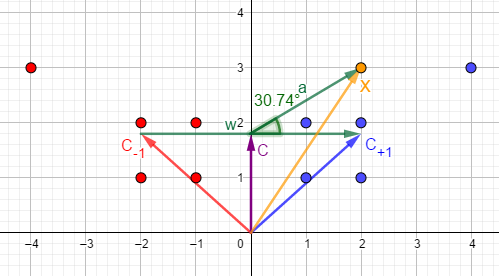
\includegraphics[width=0.5\textwidth]{kernel1.png}
\centering
\caption{Ilustração referente ao exemplo do método kernel. }
\label{kernel}
\end{figure}


\section{Postulados da Mecânica quântica}

A Mecânica Quântica é  um formalismo matemático para o desenvolvimento de teorias físicas. Por si só, ela não nos diz quais leis físicas um sistema deve obedecer, mas fornece um \textit{framework} conceitual e matemático para o desenvolvimento de tais leis. Estes postulados foram obtidos após um longo processo basicamente de tentativa e erro \cite{nielsen2000quantum}.

\subsection{Espaço de estados}

O primeiro postulado nos diz qual o `lugar'  em que a Mecânica Quântica é obedecida:
\begin{itemize}
\item \textbf{Postulado 1}: Associado a qualquer sistema físico isolado há um espaço vetorial complexo com produto interno (Espaço de Hilbert) conhecido como espaço de estados do sistema. O sistema é completamente descrito pelo seu vetor de estado, que é um vetor unitário no espaço de estados do sistema.
\end{itemize}

A Mecânica Quântica não nos diz qual o espaço de estados do sistema para um sistema físico em específico nem em qual vetor de estado o sistema está. Identificar qual é o espaço de estados para um sistema em específico é um desafio. A eletrodinâmica quântica (\textit{Quantum Electrodynamics} - QED), por exemplo, nos diz quais espaços nos fornecem uma descrição quântica dos átomos e da luz. Mas não estamos interessados em teorias complexas como QED, mas sim no framework geral fornecido pela Mecânica Quântica.

O sistema mecânico quântico mais simples e que estamos mais interessados é o \textit{qubit}. Qubit é um espaço de estados de duas dimensões. Supondo uma base ortonormal formada por $\left|0\right\rangle $ e $\left|1\right\rangle $, então um vetor de estado arbitrário no espaço pode ser descrito como: 
\begin{equation}\left|\psi\right\rangle =a\left|0\right\rangle +b\left|1\right\rangle . \end{equation}
Os coeficientes $a$ e $b$ são números complexos e, devido à condição de normalização, devem obedecer $\left|a\right|^{2}+\left|b\right|^{2}=1$.  Intuitivamente $\left|0\right\rangle $ e $\left|1\right\rangle $ são análogos dos valores $0$ e $1$ que um bit pode assumir, a diferença surge devido a superposição dos estados, isto é, o qubit pode assumir o estado $a \left|0\right\rangle + b \left|1\right\rangle $  no qual não é possível dizer se o qubit está definitivamente em um estado ou em outro. Dizemos que a combinação linear de estados  $\sum_{i}\alpha_{i}\left|\psi_{i}\right\rangle $ é uma  superposição dos estados $\left|\psi_{i}\right\rangle $ com amplitude de probabilidade $\alpha_{i}$ para o estado $\left|\psi_{i}\right\rangle $.

\subsection{Evolução}

O segundo postulado nos diz como um estado $\left|\psi\right\rangle $ varia com o tempo.
\begin{itemize}
\item \textbf{Postulado 2}: A evolução de um sistema fechado é descrita por uma transformação unitária. O estado $\left|\psi\right\rangle $ do sistema no instante $t_{1}$ é relacionado ao estado $\left|\psi'\right\rangle $ no instante $t_{2}$ por um operador unitário $U$ que depende somente dos tempos $t_{1}$ e $t_{2}$:
\end{itemize}
\begin{equation}
\left|\psi'\right\rangle =U\left|\psi\right\rangle 
. \end{equation}
Sendo que um operador unitário é definido como $UU^\dagger=U^\dagger U=\mathbb{I}$. Semelhante ao postulado anterior, a Mecânica Quântica não nos diz quais operadores $U$ descrevem a dinâmica real do mundo quântico. Somente assegura que a evolução pode ser descrita desta maneira.  Para nosso sistema de qubits qualquer operador unitário pode ser realizado em um sistema realístico.

O postulado requer que o sistema seja fechado, isto é, que só com outro sistema de forma a não mudar seu estado quântico. Apesar de todos os sistemas interagirem de alguma forma com outros sistemas, há alguns sistemas que podem ser descritos com uma boa aproximação como sendo fechados. 

\subsection{Medida quântica}
O postulado 2 descreve a evolução de um sistema fechado, ou seja, que não interage com o resto do mundo. Porém algumas vezes cientistas  desejam observar o sistema para entender o que está acontecendo, e esta interação faz com que o sistema não seja mais fechado e a partir disto, não precisa mais necessariamente obedecer o postulado 2. Para explicar o que acontece quando isto é feito, introduzimos o postulado 3 sobre os efeitos de uma medição em um sistema quântico.

\begin{itemize}
\item \textbf{Postulado 3}: As medidas quânticas são descritas por uma coleção $\left\{ M_{m}\right\} $ de operadores de medidas. Esses operadores atuam no espaço de estados que está sendo medido. O índice $m$ faz referência ao resultado que pode ocorrer no experimento. Se o estado do sistema quântico é $\left|\psi\right\rangle $ imediatamente antes da medição, a probabilidade do resultado $m$ ocorrer é dado por:
\end{itemize}
\begin{equation}
p\left(m\right)=\left\langle \psi\left|M_{m}^{\dagger}M_{m}\right|\psi\right\rangle 
. \end{equation}
E o estado do sistema após a medida é dado por:

\begin{equation}
\left|\psi'\right\rangle =\frac{M_{m}\left|\psi\right\rangle }{\sqrt{\left\langle \psi\left|M_{m}^{\dagger}M_{m}\right|\psi\right\rangle }}
. \end{equation}
Além disso, os operadores de medida satisfazem a equação completeza: $ \sum_{m}M_{m}^{\dagger}M_{m}=I.$

\subsubsection{Medidas projetivas}
Medidas projetivas são um caso especial importante do postulado 3.  Muitas aplicações de computação quântica são focadas principalmente em medidas projetivas. Além disso, pode ser equivalente ao postulado geral quando expandido com a habilidade de realizar transformações unitárias, conforme será demonstrado mais adiante com o auxílio do próximo postulado. 

\begin{itemize}
\item \textbf{Medidas projetivas}: uma medida projetiva é descrita por um observável $M$, que é um operador hermitiano no espaço de estado do sistema que está sendo observado. O observável tem a decomposição espectral:
\end{itemize}
\begin{equation}
M=\sum_{m}mP_{m}
. \end{equation}
Onde $P_{m}$ é o projetor no auto-espaço de $M$ com o autovalor $m$. Os possíveis resultados correspondem aos autovalores $m$ do observável. Então, medindo o estado $\left|\psi\right\rangle $, a probabilidade de obter o resultado $m$ é dado por:
\begin{equation}
p\left(m\right)=\left\langle \psi\left|P_{m}\right|\psi\right\rangle 
. \end{equation}
E após obtido $m$ o estado do sistema imediatamente após a medição é:
\begin{equation}
\left|\psi'\right\rangle = \frac{P_{m}\left|\psi\right\rangle }{\sqrt{p\left(m\right)}}
. \end{equation}
Medidas projetivas podem compreendidas como um caso especial do postulado 3, onde além da relação de completeza, temos as condições extras de que os operadores $M_{m}$ são Hermitianos e  $M_{m}M_{m'}=\delta_{mm'}M_{m}$. Com essas restrições, o postulado 3 se reduz as medidas projetivas definida acima. Além disto, duas nomenclaturas largamente usadas para observações merecem ênfase:
\begin{enumerate}
\item Ao invés de fornecer um observável que descreve uma medida projetiva, listam-se um conjunto de projetores ortogonais que satisfazem as condições: $\sum_{m}P_{m}=I$ e $P_{m}P_{m'}=\delta_{mm'}P_{m}.$ O correspondente observável implícito nesse caso é $M=\sum_{m}mP_{m}$.
\item Uma frase bastante usada é ``medido na base $\left|m\right\rangle $'', onde os vetores $\left|m\right\rangle $ formam uma base ortonormal. Isso significa que foi feita uma medida projetiva com os projetores: $P_{m}=\left|m\right\rangle \left\langle m\right|$.
\end{enumerate}

Tendo por exemplo uma medida projetiva em um único qubit, sendo a medida feita de um observável $Z=\left|0\right\rangle \left\langle 0\right|-\left|1\right\rangle \left\langle 1\right|$ , temos então os autovalores $+1$ e $-1$ e os autovetores $\left|0\right\rangle $ e $\left|1\right\rangle $ respectivamente. Se vamos medir no estado $\left|\psi\right\rangle =\frac{1}{\sqrt{2}}\left(\left|0\right\rangle +\left|1\right\rangle \right)$, a probabilidade de obtermos o resultado  $+1$  é $\left\langle \psi|0\right\rangle \left\langle 0|\psi\right\rangle =\frac{1}{2}$. 

\subsubsection{Fase}
``Fase''  é um termo largamente usado em Mecânica Quântica que pode ter mais de um significado dependendo do contexto. Por isso, se mostra útil abordar um par destes conceitos neste ponto. Considerando o estado  $e^{i\theta}\left|\psi\right\rangle $ onde $\left|\psi\right\rangle $ é um vetor de estado e $\theta$  um número real. Então falamos que o estado $e^{i\theta}\left|\psi\right\rangle $ é igual ao estado $\left|\psi\right\rangle $ sob um fator de fase global $e^{i\theta}$, e a estatística da medida é a mesma para ambos, ou seja, fatores de fase globais são irrelevantes para as propriedades observadas de um sistema físico. Isso é visto facilmente se supomos um operador de medida $M_m$, então a probabilidade de medirmos $m$ no estado $e^{i\theta}\left|\psi\right\rangle $ é $\left\langle \psi\left|e^{-i\theta}M_{m}^{\dagger}M_{m}e^{i\theta}\right|\psi\right\rangle =\left\langle \psi\left|M_{m}^{\dagger}M_{m}\right|\psi\right\rangle $, ou seja, o mesmo que para $\left|\psi\right\rangle $ .

Mas outro tipo de fase é a fase relativa. Considerando os estados:
\begin{equation}\frac{\left(\left|0\right\rangle +\left|1\right\rangle \right)}{\sqrt{2}}; \quad \frac{\left(\left|0\right\rangle -\left|1\right\rangle \right)}{\sqrt{2}}. \end{equation}Então a amplitude de $\left|1\right\rangle $ no primeiro e segundo estado é $\pm\frac{1}{\sqrt{2}}$, respectivamente, isto é a mesma magnitude porém com um sinal diferente. De uma maneira geral, dizemos que duas amplitudes ($a$ e $b$) diferem por uma fase relativa, se para um número $\theta$ real, temos  $a=e^{i\theta}b$.  Como a fase relativa pode variar de amplitude para amplitude,  diferentemente  da fase global não podemos considerar estes estados como fisicamente equivalentes, uma vez que as medidas estatísticas para uma propriedade observada no sistema físico será diferente para cada estado.

\subsection{Sistemas compostos}
Se estamos interessados em um sistema quântico composto, isto é, descrito por 2 ou mais sistemas físicos distintos, é o postulado 4 que descreve como um espaço de estados do sistema composto é construído a partir dos espaços de estados dos componentes do sistema.
\begin{itemize}
\item \textbf{Postulado 4}: O espaço de estados de um sistema físico composto é o produto tensorial dos espaços de estados dos componentes do sistema.
\end{itemize}

A prova de que medidas projetivas com dinâmica unitária é suficiente para implementar uma medida geral é uma boa ilustração da aplicação do postulado 4.

Suponha que temos um espaço de estados $Q$  e queremos fazer uma medida descrita pelos operadores $M_{m}$ neste espaço. Para fazer isso, introduzimos um sistema auxiliar com o espaço de estados $M$ formado por uma base ortonormal  $\left|m\right\rangle $ com uma correspondência `um-para-um' com os possíveis resultados das medidas que vamos implementar. Este sistema auxiliar pode ser tanto um mero dispositivo matemático, quanto um sistema quântico físico extra introduzido no problema. Mas independente disto, o  espaço composto é dado por $Q\otimes M$.

Sendo $\left|0\right\rangle $ um estado de $M$, definimos um operador $U$ onde:
\begin{equation}
U\left|\psi\right\rangle \left|0\right\rangle \equiv\sum_{m}M_{m}\left|\psi\right\rangle \left|m\right\rangle 
. \end{equation}
Uma observação é que há diferentes formas de representar um produto tensorial na literatura $\left|a\right\rangle \otimes\left|b\right\rangle =\left|a\right\rangle \left|b\right\rangle =\left|ab\right\rangle $. Lembrando da ortonormalidade dos estados $\left|m\right\rangle $ e a relação de completeza dos operadores $M_m$, podemos ver que o operador $U$ preserva o produto interno entre os estados na forma $\left|\psi\right\rangle \left|0\right\rangle $:
\begin{equation}
\begin{split}
\left\langle \varphi\right|\left\langle 0\right|U^{\dagger}U\left|\psi\right\rangle \left|0\right\rangle &  =\sum_{m,m'}\left(M_{m'}\left|\varphi\right\rangle \left|m'\right\rangle ,M_{m}\left|\psi\right\rangle \left|m\right\rangle \right), \\
& = \sum_{m,m'}\left(M_{m}^{\dagger}M_{m'}\left|\varphi\right\rangle \left|m'\right\rangle ,\left|\psi\right\rangle \left|m\right\rangle \right),\\
& = \sum_{m,m'}\left(M_{m}^{\dagger}M_{m'}\left|\varphi\right\rangle ,\left|\psi\right\rangle \right)\left(\left|m'\right\rangle ,\left|m\right\rangle \right),\\
& = \left(\sum_{m}M_{m}^{\dagger}M_{m}\left|\varphi\right\rangle ,\left|\psi\right\rangle \right), \\
& = \left(\left|\varphi\right\rangle ,\left|\psi\right\rangle \right), \\
& = \left\langle \varphi|\psi\right\rangle .
\end{split}
\end{equation}Então supondo que fazemos uma medida projetiva nos dois sistemas descrita pelos projetores $P_{m}=I_{Q}\otimes\left|m\right\rangle \left\langle m\right|$. A saída $m$ ocorre com a probabilidade:

\begin{equation}
\begin{split}
p\left(m\right) & =\left\langle \psi\right|\left\langle 0\right|U^{\dagger}P_{m}U\left|\psi\right\rangle \left|0\right\rangle , \\
& = \left( \sum_{m'} \left\langle \psi \right| M_{m'}^{\dagger} \left\langle m'\right|\right)\left( \mathbb{I}\otimes\left|m\right\rangle \left\langle m\right|\right)\left( \sum_{m''} M_{m''} \left|\psi\right\rangle \left|m''\right\rangle \right) \\
& =\sum_{m',m''}\left(\left\langle \psi\right|M_{m'}^{\dagger}\left\langle m'\right|\right)\left(M_{m''}\left|\psi\right\rangle \left|m\right\rangle \left\langle m|m''\right\rangle \right), \\
& =\sum_{m',m''}\left(\left\langle \psi\right|M_{m'}^{\dagger}M_{m''}\left|\psi\right\rangle \left\langle m'|m\right\rangle \left\langle m|m''\right\rangle \right), \\
& =\left\langle \psi\right|M_{m}^{\dagger}M_{m}\left|\psi\right\rangle .
\end{split}
\end{equation}

Como é dado pelo postulado 3. Após a medição, o estado do sistema é:
\begin{equation}
\begin{split}
\frac{P_{m}U\left|\psi\right\rangle \left|0\right\rangle }{\sqrt{p\left(m\right)}}& =\frac{\left(I_{Q}\otimes\left|m''\right\rangle \left\langle m''\right|\right)\left(\sum_{m}M_{m}\left|\psi\right\rangle \otimes\left|m\right\rangle \right)}{\sqrt{p\left(m\right)}}\\
 & =\sum I_{Q}{}_{m}\frac{M_{m}\left|\psi\right\rangle \otimes\left|m''\right\rangle \left\langle m''|m\right\rangle }{\sqrt{p\left(m\right)}}\\
& =\frac{M_{m}\left|\psi\right\rangle }{\sqrt{p\left(m\right)}}\otimes\left|m\right\rangle .
\end{split}
. \end{equation}
Isso implica que o estado do sistema $M$ após a medida é $\left|m\right\rangle $, o estado do sistema $Q$ é:
\begin{equation}
\left|\psi'\right\rangle =\frac{M_{m}\left|\psi\right\rangle }{\sqrt{p\left(m\right)}}
. \end{equation}
O Postulado 4 também nos ajuda a definir o entrelaçamento. Considerando por exemplo o seguinte estado de dois qubit:
\begin{equation}
\left|\psi\right\rangle =\frac{\left|00\right\rangle +\left|11\right\rangle }{\sqrt{2}}
. \end{equation}
Então este estado  não pode ser obtido por dois qubits separados $\left|a\right\rangle $ e $\left|b\right\rangle $  na forma: $\left|a\right\rangle \otimes\left|b\right\rangle $. Dizemos então que o estado de um sistema composto que tenha essa propriedade de não poder ser escrito como o produto dos estados de seus componentes, é um estado emaranhado.

\section{Computação quântica}

\subsection{Bits quânticos}
Os bits são conceitos fundamentais da computação  clássica. A computação quântica é construída em cima de um conceito análogo, o bit quântico, ou, como também é chamado, qubit.  Qubits  são objetos matemáticos conectados a objetos físicos de forma que podemos tratar aqui apenas como objetos matemáticos abstratos e termos a liberdade de construir uma teoria geral de computação quântica que não depende de um sistema específico para ser realizado.

Bits clássicos podem estar nos estados $0$ ou $1$, qubits possuem também dois estados análogos $\left|0\right\rangle $ e $\left|1\right\rangle $. Porém, como vimos anteriormente, é possível formar uma combinação linear dos estados chamada superposição, onde $\alpha$ e $\beta$ são números complexos chamados de amplitude:
\begin{equation}
\left|\psi\right\rangle =\alpha\left|0\right\rangle +\beta\left|1\right\rangle \label{qubit 1}
. \end{equation}
Os estados $\left|0\right\rangle $ e $\left|1\right\rangle $ são conhecidos como os estados da base computacional e formam uma base ortonormal para o espaço vetorial definido pelo postulado 1, onde $\left|\psi\right\rangle$ é o vetor de estado.  Enquanto o bit pode ser examinado para determinar se está no estado $0$ ou $1$, em um qubit a medida nos retorna $0$ com probabilidade $\left|\alpha\right|^{2}$ ou $1$ com probabilidade $\left|\beta\right|^{2}$. Há diferentes sistemas físicos possíveis de serem utilizados que podemos usar o conceito qubits, como por exemplo: as duas diferentes polarizações de um fóton, o alinhamento do spin nuclear em um campo magnético uniforme ou dois estados de um elétron orbitando um átomo.

Uma representação útil de pensar em qubits é usando uma representação geométrica. Como $\left|\alpha\right|^{2}+\left|\beta\right|^{2}=1$, reescrevendo a equação \ref{qubit 1}:
\begin{equation}
\left|\psi\right\rangle =e^{i\gamma}\left(\cos\left(\frac{\theta}{2}\right)\left|0\right\rangle +e^{i\varphi}\sin\left(\frac{\theta}{2}\right)\left|1\right\rangle \right)
. \end{equation}
E ignorando a fase global, pois a mesma não possui efeito observável, então:
\begin{equation}
\left|\psi\right\rangle =\cos\left(\frac{\theta}{2}\right)\left|0\right\rangle +e^{i\varphi}\sin\left(\frac{\theta}{2}\right)\left|1\right\rangle 
\label{bloch}
. \end{equation}
Então podemos definir uma esfera (Esfera de Bloch), onde os pontos são definidos por $\varphi$ e $\theta$. Essa é uma representação útil para visualizar o estado de um único qubit e pode ser visto na Figura \ref{fbloch}, porém não há uma representação equivalente para mais de um qubit. Conforme o postulado 3  para cada medição feita, alteramos o estado do sistema medido. Então, temos apenas um bit de informação sobre o estado do qubit. Logo, precisaríamos preparar infinitos qubits de forma idêntica  para determinar $\alpha$ e $\beta$ de forma exata. Isso resulta em que o estado de um qubit possui uma grande quantidade de ``informações escondidas''.

 \begin{figure}[ht]
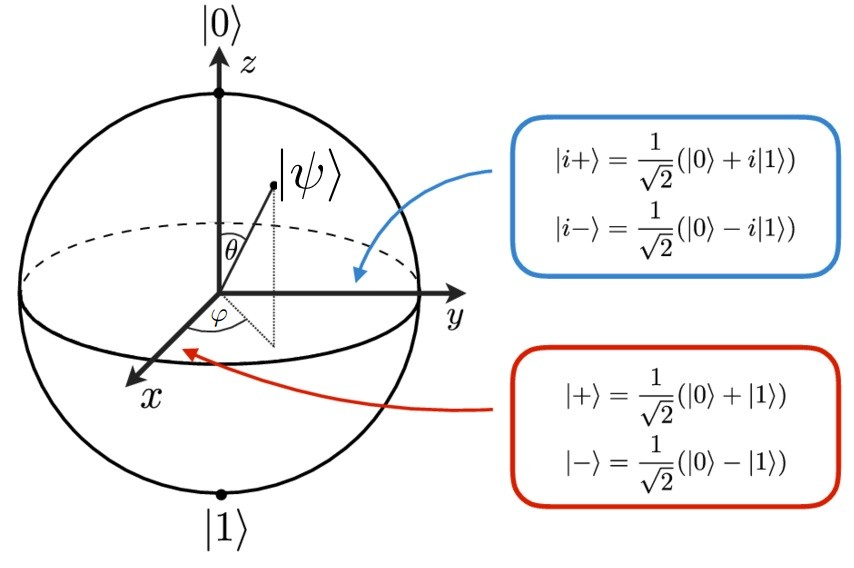
\includegraphics[width=0.5\textwidth]{bloch.jpg}
\centering
\caption{Ilustração da esfera de Bloch \cite{phdthesis}.}
\label{fbloch}
\end{figure}

O estado formado por múltiplos qubits é dado diretamente pelo postulado 4, e as medidas definidas pelo postulado 3 utilizadas na computação quântica são medidas projetivas.  Um estado importante de dois qubits é o estado de Bell ou par EPR:
\begin{equation}
\left|\psi'\right\rangle =\frac{1}{\sqrt{2}}\left(\left|00\right\rangle +\left|11\right\rangle \right)
. \end{equation}
Esse estado tem a propriedade de que após a medição do primeiro qubit, que tem probabilidade de $1/2$ para cada resultado, o segundo está definido e será sempre igual ao primeiro resultado. Portanto dizemos que o resultado está correlacionado, e essa correlação é mais forte do que jamais  poderia existir entre sistemas clássicos.  O estado quântico de um sistema com $n$ qubits é determinado por $2^{n}$ amplitudes. Para $n=500$ há mais amplitudes que átomos no universo, informação que é impossível ser armazenada em um computador clássico. Porém a natureza manipula essa enorme quantidade de dados.

\subsection{Operadores unitários de qubit }
Já discutimos que o conceito fundamental da computação quântica são os vetores de estado chamados qubits e a base no espaço de Hilbert é  a  base computacional (postulado 1).  As medidas realizadas na computação quântica são medidas projetivas (postulado 3) e qubits individuais podem compor um sistema maior de múltiplos qubits  (postulado 4), porém nos falta descrever de como o sistema evolui no tempo (postulado 2), e isto é feito com operadores unitários.

Mudanças que ocorrem em um estado quântico genérico podem ser descritas usando a linguagem da computação quântica, que de uma maneira análoga a um computador clássico que é construído por um circuito elétrico, um computador quântico é construído a partir de um circuito quântico contendo operadores quânticos  para carregar e manipular a informação quântica. 

O operador clássico NOT é definido pela tabela verdade onde $0\rightarrow 1$ e $1\rightarrow 0$. Podemos construir um análogo quântico, porém sem esquecer que comportamento linear é uma propriedade geral da Mecânica Quântica bem motivada empiricamente, o comportamento não linear poderia levar a aparente paradoxos. Um meio conveniente de representar um operador NOT quântico é na forma matricial:
\begin{equation}
X\equiv\left[\begin{array}{cc}
0 & 1\\
1 & 0
\end{array}\right]
. \end{equation}
E se o estado quântico $\alpha\left|0\right\rangle +\beta\left|1\right\rangle $, que pode ser denotado vetorialmente como $\left[\begin{array}{cc}
\alpha & \beta\end{array}\right]^{T},$  então:

\begin{equation}
X\left[\begin{array}{c}
\alpha\\
\beta
\end{array}\right]=\left[\begin{array}{c}
\beta\\
\alpha
\end{array}\right]
. \end{equation}
O que resulta em um comportamento análogo ao NOT clássico, $\alpha \rightarrow \beta$  e $\beta \rightarrow \alpha$. Então a evolução de sistemas quânticos de um único qubit pode ser descrita por operadores unitários ($U^{\dagger}U=I$)  que possuem uma descrição matricial por matrizes $2\times2$ . É válido aqui relembrar que  qualquer matriz unitária é válida. 

Apesar de haver infinitas matrizes $2\times 2$, um  operador unitário de um qubit arbitrário pode ser decomposto como produto de rotações em diferentes planos e um deslocamento de fase global (uma constante multiplicando como $e^{i\alpha}$).  Isso é, uma matriz unitária $2 \times 2$ arbitrária  pode ser decomposta como:
\begin{equation}
U=e^{i\alpha}\left[\begin{array}{cc}
e^{-i\beta/2} & 0\\
0 & e^{i\beta/2}
\end{array}\right]\left[\begin{array}{cc}
\cos\left(\frac{\gamma}{2}\right) & -\sin\left(\frac{\gamma}{2}\right)\\
\sin\left(\frac{\gamma}{2}\right) & \cos\left(\frac{\gamma}{2}\right)
\end{array}\right]\left[\begin{array}{cc}
e^{-i\delta/2} & 0\\
0 & e^{i\delta/2}
\end{array}\right]
. \end{equation}
Onde $\alpha$,$\beta$, $\gamma$ e $\delta$  são valores reais. Essa é uma prescrição exata para qualquer operador unitário de um qubit. Não precisamos ser capazes de trabalharmos com esses operadores para valores arbitrários, podemos construir aproximações arbitrariamente boas para esses operadores usando somente alguns valores especiais fixos. Então uma computação arbitrária de um único qubit pode ser feita com um conjunto finito de operadores, e mais geral ainda, uma computação arbitrária de qualquer número de qubits pode ser gerada com um conjunto finito de operadores que são considerados universais para a computação quântica. Para obter esse conjunto universal, precisamos ver operadores para múltiplos qubits.

\subsection{Operadores de múltiplo qubits}

O protótipo dos operadores lógicos quânticos de múltiplos qubits, é o CNOT (NOT Controlado,  que também é chamado de X controlado, ou CX). A ação do operador  é descrita a seguir. O operador tem duas entradas, se o qubit de controle é $0$, o qubit alvo permanece inalterado, mas se o qubit de controle é 1, o qubit alvo é invertido, isto é:

\begin{equation}
\begin{split}
\left|00\right\rangle \rightarrow\left|00\right\rangle, \\
\left|01\right\rangle \rightarrow\left|01\right\rangle,  \\
\left|10\right\rangle \rightarrow\left|11\right\rangle,  \\
\left|11\right\rangle \rightarrow\left|10\right\rangle. \\
\end{split}
\end{equation}
Outra maneira de descrever, é como uma generalização do operador clássico XOR: $ \left|A,B\right\rangle \rightarrow\left|A,A\oplus B\right\rangle $,  onde $\oplus$ é uma adição de módulo 2. Sua representação matricial é dada por:
\begin{equation}
U_{CN}=\left[\begin{array}{cccc}
1 & 0 & 0 & 0\\
0 & 1 & 0 & 0\\
0 & 0 & 0 & 1\\
0 & 0 & 1 & 0
\end{array}\right]
. \end{equation}
Conforme determinado pelo postulado 2,  $U_{CN}$ é um operador unitário. Operadores unitários de qubits e CNOT são os protótipos para todos os outros operadores. Então qualquer operador lógico de múltiplos qubits pode ser construído utilizando CNOT e operadores unitários de 1 qubit. Isso é análogo à universalidade do operador NAND na computação clássica. Porém nem todas operações clássicas possuem análogos quânticos diretos como o NOT. O NAND, por exemplo, é irreversível, ou seja, há uma perda de informação inevitável. Porém operadores quânticos são sempre inversíveis.

A  escolha de $\left|0\right\rangle $ e $\left|1\right\rangle $ como base computacional representa somente uma das muitas possíveis escolhas de base de estados para um qubit. Porém a Mecânica Quântica permite maior versatilidade, sendo possível trabalharmos com outras bases. 

\subsection{Circuitos quânticos}

Circuitos quânticos são lidos da esquerda para a direita  correspondendo a passagem do tempo. Cada linha representa um qubit ao longo do tempo.  É convencional assumir que o estado de entrada do circuito consiste de todos qubits em $\left|0\right\rangle $. %Um circuito simples e útil é o responsável por realizar a operação conhecida como swap: trocar o estado entre dois qubits. 

Como sugerido anteriormente, tem algumas características de circuitos clássicos que não estão presentes em circuitos quânticos: Primeiro de tudo, não  há  loops, circuitos quânticos são acíclicos. Também temos que as linhas não podem ser condensadas (operação conhecida como FANIN em circuitos clássicos). E por fim, também não pode ser feito cópias dos bits (operação conhecida como FANOUT). Antes de avançar,  é conveniente introduzirmos uma nova notação: Qubits de controle são identificados como pontos pretos, e medidas são representados por um medidor. Como o nome sugere, essa operação representa uma medição, ou seja, converte o estado $\left|\psi\right\rangle =\alpha\left|0\right\rangle +\beta\left|1\right\rangle $  de um único qubit em um bit probabilístico clássico (que é diferenciado de um qubit por uma linha dupla) onde é $0$ com probabilidade $\left|\alpha\right|^{2}$ e $1$ com probabilidade $\left|\beta\right|^{2}$.

\begin{figure}[ht]
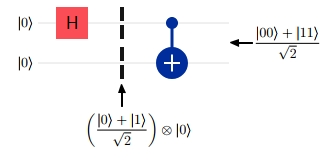
\includegraphics[width=0.5\textwidth]{par_epr.jpg}
\centering
\caption{Circuíto quântico que resulta em um estado Bell.}
\label{bell}
\end{figure}

\subsubsection{Exemplo: Estado de Bell}
Podemos construir um estado de Bell em um sistema com 2 qubits, aplicando um operador Hadamard no primeiro qubit, e então usando este mesmo qubit de controle para um CNOT  que tem como alvo o segundo qubit. Sendo o operador de Hadamard responsável por criar sobreposição, ele é definido como
\begin{equation}
\begin{split}
H &\equiv \left[\begin{array}{cc}
1 & 1\\
1 & -1
\end{array}\right] \frac{1}{\sqrt{2}}
\end{split}
. \end{equation}
Para o estado inicial $\left|00\right\rangle $ após aplicarmos o operador Hadamard, o estado do sistema vai para $\left(\left|0\right\rangle +\left|1\right\rangle \right)\left|0\right\rangle /\sqrt{2}$, e então com o CNOT ficamos com $\left(\left|00\right\rangle +\left|11\right\rangle \right)/\sqrt{2}$. Este estado é conhecido como estado de Bell (ou estado EPR, ou ainda par EPR) e está ilustrado na figura \ref{bell}.

\subsubsection{Exemplo: Teleportação quântica}

Teleportação quântica é uma técnica para mover estados quânticos, mesmo sem  enviar os qubits diretamente. Muitas ideias da computação quântica são entendidas melhor usando metáforas envolvendo duas partes, popularmente chamadas de Alice e Bob. Então a questão pode ser formulada da seguinte maneira: temos um par de qubits no estado de Bell, Alice e Bob possuem cada um qubit desse par e encontram-se separados. Alice tem a missão de entregar um qubit $\left|\psi\right\rangle =\alpha\left|0\right\rangle +\beta\left|1\right\rangle $ ao Bob, porém ela não conhece o estado do qubit e só pode enviar informação clássica ao Bob.

Isso pode ser feito da maneira descrita  a seguir, lembrando que o sistema todo é composto de três qubits, o $\left|\psi\right\rangle $ que Alice deseja enviar para Bob e o par $\left|\beta_{00}\right\rangle $ compartilhado entre ambos. O estado inicial $\left|\psi_{0}\right\rangle $ é então:
\begin{equation}
\begin{split}
\left|\psi_{0}\right\rangle & =\left|\psi\right\rangle \left|\beta_{00}\right\rangle \\
& =\left[\alpha\left|0\right\rangle \left(\left|00\right\rangle +\left|11\right\rangle \right)+\beta\left|1\right\rangle \left(\left|00\right\rangle +\left|11\right\rangle \right)\right]\frac{1}{\sqrt{2}}.
\end{split}
 \end{equation}
Convenientemente, vamos  denotar que os primeiros dois qubits à esquerda pertencem a Alice e o terceiro ao Bob. Então Alice aplica um operador CNOT nos seus dois qubits, usando o qubit que quer enviar como o qubit de controle. Temos assim:
\begin{equation}
\left|\psi_{1}\right\rangle =\left[\alpha\left|0\right\rangle \left(\left|00\right\rangle +\left|11\right\rangle \right)+\beta\left|1\right\rangle \left(\left|10\right\rangle +\left|01\right\rangle \right)\right]\frac{1}{\sqrt{2}}
. \end{equation}
O próximo passo da Alice é aplicar o operador Hadamard no primeiro qubit:
\begin{equation}
\begin{split}
\left|\psi_{2}\right\rangle & =\frac{1}{2}\left[\left|00\right\rangle \left(\alpha\left|0\right\rangle +\beta\left|1\right\rangle \right)+\left|01\right\rangle \left(\alpha\left|1\right\rangle +\beta\left|0\right\rangle \right)+\left|10\right\rangle \left(\alpha\left|0\right\rangle -\beta\left|1\right\rangle \right)+\left|11\right\rangle \left(\alpha\left|1\right\rangle -\beta\left|0\right\rangle \right)\right] \\
\end{split}
\label{psi2A}
. \end{equation}
Nota-se que a expressão se divide em 4 termos. No primeiro termo, Alice possui os qubits no estado $\left|00\right\rangle $ e Bob no estado $\alpha\left|0\right\rangle +\beta\left|1\right\rangle $, analisando de maneira similar os outros termos:
\begin{equation}
\begin{split}
\left|00\right\rangle \rightarrow\psi_{3}\equiv\alpha\left|0\right\rangle +\beta\left|1\right\rangle , \\
\left|01\right\rangle \rightarrow\psi_{3} \equiv\alpha\left|1\right\rangle +\beta\left|0\right\rangle , \\
\left|10\right\rangle \rightarrow\psi_{3}  \equiv\alpha\left|0\right\rangle -\beta\left|1\right\rangle, \\
\left|11\right\rangle \rightarrow\psi_{3} \equiv\alpha\left|1\right\rangle -\beta\left|0\right\rangle .
\end{split}
\end{equation}
Então uma vez que Bob saiba qual foi a medida da Alice (fato que impede que a informação seja transmitida mais rápido que a luz), ele pode ``corrigir''  seu estado e recuperar $\left|\psi\right\rangle $ aplicando um operador unitário apropriado. Já vimos que para o caso $\left|00\right\rangle $ não é necessário aplicar nenhuma operação (ou aplicar o operador identidade), de maneira análoga para os outros casos:
\begin{equation}
\begin{split}
\left|00\right\rangle  & \rightarrow \mathbb{I}, \\
\left|01\right\rangle  & \rightarrow X, \\
\left|10\right\rangle  & \rightarrow Z,\\
\left|11\right\rangle  & \rightarrow ZX. \\
\end{split}
\end{equation}Onde o operador $Z$ é definido como:
\begin{equation}
\begin{split}
Z &\equiv\left[\begin{array}{cc}
1 & 0\\
0 & -1
\end{array}\right] \\
\end{split}
. \end{equation}
Então Bob precisa de maneira genérica aplicar o operador $Z^{M_{1}}X^{M_{2}}$, onde $M_i$ indica o bit $i$ na string $\left|bb\right\rangle $ (contando da esquerda para a direita). 

\section{Algoritmo quântico}

\subsection{Computação clássica em um computador quântico}

Qualquer circuito clássico pode ser substituído por um circuito equivalente somente com elementos reversíveis, usando um operador conhecido como porta de Toffoli. O operador de Toffoli tem três bits, porém o terceiro bit  (bit alvo)  é invertido somente se os outros dois bits  (bits de controle) são 1, $\left(a,b,c\right)\rightarrow\left(a,b,c\oplus ab\right)$.  Operador Toffoli pode ser usado pra simular operadores NAND, FANOUT.  Com isso podemos simular qualquer circuito clássico com um circuito reversível equivalente. Se desejamos simular um computador clássico não determinístico, isto é, com a habilidade de gerar bits aleatórios, preparamos um qubit no estado $\left|0\right\rangle $ e usamos um operador de Hadamard, após a medição ser realizada, tem 50/50 de probabilidade de medir $\left|0\right\rangle $ ou $\left|1\right\rangle $.

Porém a habilidade de simular computadores clássicos é apenas uma característica dos computadores quânticos. Funções muito mais poderosas podem ser computadas usando qubits e operadores quânticos, como veremos nas seções a seguir.

% POSSO INSERIR AQUI O PROBLEMA DA LINEARIDDE ?

\subsection{Paralelismo quântico}

De forma simplificada, o paralelismo quântico permite que computadores quânticos avaliem a função $f\left(x\right)$ para diferentes valores de $x$ simultaneamente. Isto é, supondo uma função com o domínio e imagem de um bit ( $f\left(x\right):\left\{ 0,1\right\} \rightarrow\left\{ 0,1\right\} $), uma maneira conveniente de computar essa função é considerar um computador quântico de dois qubits que inicia no estado $\left|x,y\right\rangle $ e com uma sequência de operadores então termina no  estado $\left|x,y\oplus f\left(x\right)\right\rangle $.

Vamos chamar o operador responsável pela transformação $\left|x,y\right\rangle \rightarrow\left|x,y\oplus f\left(x\right)\right\rangle $, de $U_{f}$, e o primeiro registo de dado, e o segundo de alvo. Se $y=0$, então o estado final é simplesmente $\left|x,f\left(x\right)\right\rangle $.  Considerando então um sistema onde foi aplicado o operador de Hadamard no primeiro qubit, o estado é então $
\frac{1}{\sqrt{2}}\left(\left|0,0\right\rangle +\left|1,0\right\rangle \right)
$, e após aplicar o operador $U_{f}$ temos:
\begin{equation}
\frac{1}{\sqrt{2}}\left(\left|0,f\left(0\right)\right\rangle +\left|1,f\left(1\right)\right\rangle \right)
. \end{equation}
Os diferentes termos contém informações de $f\left(0\right)$ e $f\left(1\right)$. Dessa forma é como se tivéssemos avaliados $f\left(x\right)$ simultaneamente para ambos os valores de $x$. Esse processo pode ser generalizado para funções de quantidades arbitrárias de bits, usando uma operação geral chamada de transformada de Hadamard (ou Walsh-Hadamard). Esta transformada não é nada além de $n$ operadores Hadamard atuando paralelamente em $n$ qubits ($H^{\otimes n}$).  

Então, o paralelismo quântico de uma função de $n$ bits de entrada e um bit de saída, pode ser feito da seguinte maneira: 
\begin{enumerate}
\item Preparamos o estado de $n+1$ qubits: $\left|0\right\rangle ^{\otimes n}\left|0\right\rangle $ ;
\item Aplicamos o Hadamard paralelo aos $n$ qubits: $\frac{1}{\sqrt{2^{n}}}\sum_{x}\left|x\right\rangle \left|0\right\rangle $;
\item Implementamos $U_{f}$ :$\frac{1}{\sqrt{2^{n}}}\sum_{x}\left|x\right\rangle \left|f\left(x\right)\right\rangle $.
\end{enumerate}

Porém a medição nos retorna apenas um dos resultados de $f\left(x\right)$, para um único valor de $x$. Dessa maneira a computação quântica requer mais do que apenas paralelismo quântico, precisamos extrair informação de mais do que um valor de $f\left(x\right)$. Vvamos ver dois exemplos de como isso pode ser feito.

\subsection{Algoritmo de Deutsch}

A versão que vamos abordar é uma versão simplificada e melhorada da versão original \cite{nielsen2000quantum}. Como feito anteriormente, primeiro usamos o operador de Hadamard  para preparar o primeiro qubit ($x$) em um estado de superposição: $\left(\left|0\right\rangle +\left|1\right\rangle \right)\frac{1}{\sqrt{2}}$, mas agora preparamos o segundo qubit ($y$)  também em uma superposição: $\left(\left|0\right\rangle -\left|1\right\rangle \right)/\frac{1}{\sqrt{2}}$ , o que pode ser feito aplicando o Hadamard em um estado $\left|1\right\rangle $.  Então considerando o seguinte estado inicial: 
\begin{equation}
\left|\psi_{0}\right\rangle =\left(\left|0\right\rangle \right)\otimes\left(\left|1\right\rangle \right)
\label{anterior0}
. \end{equation}
Temos, depois de aplicar o operador Hadamard em ambos os qubits:
\begin{equation}
\begin{split}
\left|\psi_{1}\right\rangle & =\left[\frac{\left(\left|0\right\rangle +\left|1\right\rangle \right)}{\sqrt{2}}\right]\otimes\left[\frac{\left(\left|0\right\rangle -\left|1\right\rangle \right)}{\sqrt{2}}\right] \\
& =\sum_{x\in\left\{ 0,1\right\} ^{1}}\left[\frac{\left|x\right\rangle }{\sqrt{2}}\left(\frac{\left|0\right\rangle -\left|1\right\rangle }{\sqrt{2}}\right)\right]. \\
\end{split}
\label{anterior}
\end{equation}
Aplicando o operador responsável pela transformação  $\left|x,y\right\rangle \rightarrow\left|x,y\oplus f\left(x\right)\right\rangle $ obtemos:
\begin{equation}
\begin{split}
\left|\psi_{2}\right\rangle & =\left[\left|0\right\rangle \left(\left|0\oplus f\left(0\right)\right\rangle -\left|1\oplus f\left(0\right)\right\rangle \right)+\left|1\right\rangle \left(\left|0\oplus f\left(1\right)\right\rangle -\left|1\oplus f\left(1\right)\right\rangle \right)\right]\frac{1}{2} \\
&  =\left[\left|0\right\rangle \left(\left|f\left(0\right)\right\rangle -\left|1\oplus f\left(0\right)\right\rangle \right)+\left|1\right\rangle \left(\left|f\left(1\right)\right\rangle -\left|1\oplus f\left(1\right)\right\rangle \right)\right].\frac{1}{2} \\
\end{split}
\end{equation}
Agora precisamos analisar as diferentes combinações possíveis de valores para $f\left(0\right)$  e $f\left(1\right)$. Começando com o caso em que $f\left(0\right)=f\left(1\right)$:
\begin{equation}
\left|\psi_{2}\right\rangle =\left\{ \begin{array}{cc}
\left[+\left|0\right\rangle \left(\left|0\right\rangle -\left|1\right\rangle \right)+\left|1\right\rangle \left(\left|0\right\rangle -\left|1\right\rangle \right)\right]\frac{1}{2}, & f\left(0\right)=0\\
\left[-\left|0\right\rangle \left(\left|0\right\rangle -\left|1\right\rangle \right)-\left|1\right\rangle \left(\left|0\right\rangle -\left|1\right\rangle \right)\right]\frac{1}{2}, & f\left(0\right)=1
\end{array}\right.
. \end{equation}
O segundo conjunto de situações é quando $f\left(0\right)\neq f\left(1\right)$:
\begin{equation}
\left|\psi_{2}\right\rangle =\left\{ \begin{array}{cc}
\left[+\left|0\right\rangle \left(\left|0\right\rangle -\left|1\right\rangle \right)-\left|1\right\rangle \left(\left|0\right\rangle -\left|1\right\rangle \right)\right]\frac{1}{2}, & f\left(0\right)=0\\
\left[-\left|0\right\rangle \left(\left|1\right\rangle -\left|0\right\rangle \right)+\left|1\right\rangle \left(\left|0\right\rangle -\left|1\right\rangle \right)\right]\frac{1}{2}, & f\left(0\right)=1
\end{array}\right.
. \end{equation}
Podemos generalizar então:
\begin{equation}
\begin{split}
\left|\psi_{2}\right\rangle & =\left[\left(-1\right)^{f\left(0\right)}\left|0\right\rangle \left(\left|0\right\rangle -\left|1\right\rangle \right)+\left(-1\right)^{f\left(1\right)}\left|1\right\rangle \left(\left|0\right\rangle -\left|1\right\rangle \right)\right]\frac{1}{2} \\
 & = \sum_{x\in\left\{ 0,1\right\} ^{1}}\left[\frac{\left(-1\right)^{f\left(x\right)}\left|x\right\rangle }{\sqrt{2}}\left(\frac{\left|0\right\rangle -\left|1\right\rangle }{\sqrt{2}}\right)\right]
\end{split}
\label{anterior1}
. \end{equation}
Estado que tem a seguinte representação vetorial:
\begin{equation}
\left|\psi_{2}\right\rangle =\left[\begin{array}{cccc}
\left(-1\right)^{f\left(0\right)} & -\left(-1\right)^{f\left(0\right)} & \left(-1\right)^{f\left(1\right)} & -\left(-1\right)^{f\left(1\right)}\end{array}\right]^{T}\frac{1}{2}
. \end{equation}
Agora vamos aplicar o Hadamard no primeiro qubit. Lembrando que para um espaço de $2$ qubits precisamos então fazer um produto tensorial com uma matriz identidade:
\begin{equation}
H\left(0\right)=\frac{1}{\sqrt{2}}\left[\begin{array}{cc}
1 & 1\\
1 & -1
\end{array}\right]\otimes\left[\begin{array}{cc}
1 & 0\\
0 & 1
\end{array}\right]=\left[\begin{array}{cccc}
1 & 0 & 1 & 0\\
0 & 1 & 0 & 1\\
1 & 0 & -1 & 0\\
0 & 1 & 0 & -1
\end{array}\right]\frac{1}{\sqrt{2}}
. \end{equation}
Então aplicando:
\begin{equation}
\left|\psi_{3}\right\rangle =\frac{1}{\sqrt{2}}\left[\begin{array}{cccc}
1 & 0 & 1 & 0\\
0 & 1 & 0 & 1\\
1 & 0 & -1 & 0\\
0 & 1 & 0 & -1
\end{array}\right]\left[\begin{array}{c}
\left(-1\right)^{f\left(0\right)}\\
-\left(-1\right)^{f\left(0\right)}\\
\left(-1\right)^{f\left(1\right)}\\
-\left(-1\right)^{f\left(1\right)}
\end{array}\right]\frac{1}{2} 
=
\left[\begin{array}{c}
\left(-1\right)^{f\left(0\right)}+\left(-1\right)^{f\left(1\right)}\\
-\left(-1\right)^{f\left(0\right)}-\left(-1\right)^{f\left(1\right)}\\
\left(-1\right)^{f\left(0\right)}-\left(-1\right)^{f\left(1\right)}\\
-\left(-1\right)^{f\left(0\right)}+\left(-1\right)^{f\left(1\right)}
\end{array}\right]\frac{1}{2\sqrt{2}}
. \end{equation}
Temos novamente os 4 casos de valores de $f\left(0\right)$ e $f\left(1\right)$, para analisar.  Começando com $f\left(0\right)=f\left(1\right)$:
\begin{equation}
\begin{split}
\left|\psi_{3}\right\rangle & =\left\{ \begin{array}{cc}
\left[\begin{array}{cccc}
1 & -1 & 0 & 0\end{array}\right]^{T}\frac{1}{\sqrt{2}} & ,f\left(0\right)=0\\
\left[\begin{array}{cccc}
-1 & 1 & 0 & 0\end{array}\right]^{T}\frac{1}{\sqrt{2}} & ,f\left(0\right)=1
\end{array}\right. \\
& =\left\{ \begin{array}{cc}
+\left(\left|00\right\rangle -\left|01\right\rangle \right)\frac{1}{\sqrt{2}} & ,f\left(0\right)=0\\
-\left(\left|00\right\rangle -\left|01\right\rangle \right)\frac{1}{\sqrt{2}} & ,f\left(0\right)=1
\end{array}\right. \\
& = \pm\left(\left|00\right\rangle -\left|01\right\rangle \right)\frac{1}{\sqrt{2}} \\
& =\pm\left|0\right\rangle \left(\left|0\right\rangle -\left|1\right\rangle \right)\frac{1}{\sqrt{2}}.
\end{split}
\end{equation}
E se $f\left(0\right)\neq f\left(1\right)$:
\begin{equation}
\begin{split}
\left|\psi_{3}\right\rangle & =\left\{ \begin{array}{cc}
\left[\begin{array}{cccc}
0 & 0 & 1 & -1\end{array}\right]^{T}\frac{1}{\sqrt{2}} & ,f\left(0\right)=0\\
\left[\begin{array}{cccc}
0 & 0 & -1 & 1\end{array}\right]^{T}\frac{1}{\sqrt{2}} & ,f\left(0\right)=1
\end{array}\right. \\
& =\left\{ \begin{array}{cc}
+\left(\left|10\right\rangle -\left|11\right\rangle \right)\frac{1}{\sqrt{2}} & ,f\left(0\right)=0\\
-\left(\left|10\right\rangle -\left|11\right\rangle \right)\frac{1}{\sqrt{2}} & ,f\left(0\right)=1
\end{array}\right. \\
& = \pm\left(\left|10\right\rangle -\left|11\right\rangle \right)\frac{1}{\sqrt{2}} \\
& =\pm\left|1\right\rangle \left(\left|0\right\rangle -\left|1\right\rangle \right)\frac{1}{\sqrt{2}}.
\end{split}
\end{equation}
Podemos simplificar o resultado lembrando que:
\begin{equation}
f\left(0\right)\oplus f\left(1\right)=\left\{ \begin{array}{cc}
0, & f\left(0\right)=f\left(1\right)\\
1, & f\left(0\right)\neq f\left(1\right)
\end{array}\right.
. \end{equation}
Então:
\begin{equation}
\left|\psi_{3}\right\rangle =\pm\left|f\left(0\right)\oplus f\left(1\right)\right\rangle \left(\left|0\right\rangle -\left|1\right\rangle \right)\frac{1}{\sqrt{2}}
. \end{equation}
O sinal $\pm$ é irrelevante, pois a medida será do quadrado dos coeficientes. Dessa maneira podemos determinar a propriedade global $f\left(0\right)\oplus f\left(1\right)$ com apenas uma medida de $f\left(x\right)$, enquanto caso tivéssemos um aparato clássico precisaríamos ao menos de 2 medições. A essência do desenvolvimento de muitos algoritmos quânticos é realizar uma escolha inteligente da função e da transformação final que permita uma determinação eficiente da informação global útil sobre a função, informação essa que não poderia ser obtida rapidamente em um computador clássico.

\subsection{O algoritmo de Deutsch-Jozsa}
O algoritmo de Deutsch é um caso simples de um caso mais geral, que vamos chamar de algoritmo de Deutsch-Jozsa. A aplicação é conhecida como problema de Deustch e pode ser descrito como um jogo:

Os dois protagonistas são Alice em Amsterdam e Bob em Boston, a Alice seleciona um número $x$ entre $0$ e $2^{n}-1$ e envia uma carta para o Bob. Então Bob calcula alguma função $f\left(x\right)$  e responde Alice com o resultado $0$ ou $1$. Porém Bob prometeu usar uma função que é um dos dois tipos:  ou $f\left(x\right)$  é constante para todos valores de $x$ ou  $f\left(x\right)$  é perfeitamente balanceado, isto é, 0 para exatamente metade dos casos possíveis e 1 para a outra metade. O objetivo da Alice é determinar com certeza se Bob escolheu uma função constante ou balanceada.

No caso clássico, Alice pode enviar ao Bob apenas um valor de $x$  por carta. No pior cenário será necessário ao menos $\frac{2^{n}}{2}+1$ requisições ao Bob, uma vez que pode receber $\frac{2^{n}}{2}$ respostas com o valor $0$ antes de receber uma com o valor $1$ (ou vice-versa). Em cada carta, Alice envia $n$ bits de informação. Mas se podem trocar qubits e Bob usa uma transformação unitária $U_f$ para calcular $f\left(x\right)$, Alice pode alcançar seu objetivo com apenas uma correspondência usando o algoritmo que iremos discutir na sequência.

Semelhante ao algoritmo de Deutsch, Alice deve ter $n$ qubits para armazenar $x$ (registradores de dados) e um único qubit no qual o Bob vai guardar a resposta (registrador alvo). Alice vai preparar os qubits em um estado de superposição, então Bob deve avaliar $f\left(x\right)$ usando paralelismo quântico, deixar o resultado no qubit de resposta e devolver a Alice, após isto, Alice então interfere nos estados de superposição usando a transformada de Hadamard nos registradores de dados e termina realizando uma medição adequada para determinar se $f$ é constante ou balanceado.

De forma análoga ao caso anterior, equação (\ref{anterior0}), começamos com o estado inicial:
\begin{equation}
\left|\psi_{0}\right\rangle =\left|0\right\rangle ^{\otimes n}\left|1\right\rangle 
. \end{equation}
Então após aplicarmos os operadores de Hadamard, análogo também à equação (\ref{anterior}):
\begin{equation}
\left|\psi_{1}\right\rangle =\sum_{x\in\left\{ 0,1\right\} ^{n}}\frac{\left|x\right\rangle }{\sqrt{2^{n}}}\left[\frac{\left|0\right\rangle -\left|1\right\rangle }{\sqrt{2}}\right]
. \end{equation}E como demonstramos anteriormente, na equação (\ref{anterior1}), após aplicarmos o operador $U_{f}$, o estado resultante pode ser generalizado como:
\begin{equation}
\left|\psi_{2}\right\rangle =\sum_{x\in\left\{ 0,1\right\} ^{n}}\frac{\left(-1\right)^{f\left(x\right)}\left|x\right\rangle }{\sqrt{2^{n}}}\left[\frac{\left|0\right\rangle -\left|1\right\rangle }{\sqrt{2}}\right]
. \end{equation}
Nesse momento Alice tem um conjunto de qubits em que o resultado da avaliação da função do Bob está armazenado na amplitude do estado do qubit em superposição. Agora Alice pode usar a interferência nos termos em superposição, usando a transformação de Hadamard nos registradores dados. Antes de calcularmos a aplicação da transformada de Hadamard nos registradores de dados, primeiro vamos calcular a transformada em um único estado $\left|x\right\rangle $.  Considerando apenas um qubit:
\begin{equation}
\begin{split}
H\left|0\right\rangle & =\frac{1}{\sqrt{2}}\left(\left|0\right\rangle +\left|1\right\rangle \right)=\sum_{z\in\left\{ 0,1\right\} ^{1}} \frac{\left|z\right\rangle }{\sqrt{2}},\\
H\left|1\right\rangle & =\frac{1}{\sqrt{2}}\left(\left|0\right\rangle -\left|1\right\rangle \right)=\sum_{z\in\left\{ 0,1\right\} ^{1}} \left(-1\right)^{z}\frac{\left|z\right\rangle }{\sqrt{2}}.
\end{split}
\end{equation}Então podemos generalizar para um qubit:
\begin{equation}
H\left|x\right\rangle =\sum_{z\in\left\{ 0,1\right\} ^{1}}\left(-1\right)^{x\cdot z}\frac{\left|z\right\rangle }{\sqrt{2}}
. \end{equation}
Para 2 qubits, a transformada de Hadamard é dada por:
\begin{equation}
H^{\otimes2}=\frac{1}{\sqrt{2}}\left[\begin{array}{cc}
1 & 1\\
1 & -1
\end{array}\right]\otimes\left[\begin{array}{cc}
1 & 1\\
1 & -1
\end{array}\right]\frac{1}{\sqrt{2}}=\left[\begin{array}{cccc}
1 & 1 & 1 & 1\\
1 & -1 & 1 & -1\\
1 & 1 & -1 & -1\\
1 & -1 & -1 & 1
\end{array}\right]
. \end{equation}
E então:
\begin{equation}
\begin{split}
H^{\otimes2}\left|00\right\rangle & =\frac{1}{2}\left(\left|00\right\rangle +\left|01\right\rangle +\left|10\right\rangle +\left|11\right\rangle \right)=\sum_{z_{0},z_{1}\in\left\{ 0,1\right\} ^{1}} \frac{\left|z_{0},z_{1}\right\rangle }{{2}}, \\
H^{\otimes2}\left|01\right\rangle & =\frac{1}{2}\left(\left|00\right\rangle -\left|01\right\rangle +\left|10\right\rangle -\left|11\right\rangle \right)=\sum_{z_{0},z_{1}\in\left\{ 0,1\right\} ^{1}} \frac{\left(-1\right)^{z_{1}}\left|z_{0},z_{1}\right\rangle }{2}, \\
H^{\otimes2}\left|10\right\rangle & =\frac{1}{2}\left(\left|00\right\rangle +\left|01\right\rangle -\left|10\right\rangle -\left|11\right\rangle \right)=\sum_{z_{0},z_{1}\in\left\{ 0,1\right\} ^{1}} \frac{\left(-1\right)^{z_{0}}\left|z_{0},z_{1}\right\rangle }{2}, \\
H^{\otimes2}\left|11\right\rangle & =\frac{1}{2}\left(\left|00\right\rangle -\left|01\right\rangle -\left|10\right\rangle +\left|11\right\rangle \right)=\sum_{z_{0},z_{1}\in\left\{ 0,1\right\} ^{1}} \frac{\left(-1\right)^{z_{0}+z_{1}}\left|z_{0},z_{1}\right\rangle }{2}.
\end{split}
\end{equation}
Por sua vez, pode ser generalizado como:
\begin{equation}
\begin{split}
H^{\otimes2}\left|x_{0},x_{1}\right\rangle & =\sum_{z_{0},z_{1}\in\left\{ 0,1\right\} ^{1}}\frac{\left(-1\right)^{x_{0}\cdot z_{0}+x_{1}\cdot z_{1}}\left|z_{0},z_{1}\right\rangle }{2}, \\
H^{\otimes2}\left|x\right\rangle & =\sum_{z\in\left\{ 0,1\right\} ^{2}}\frac{\left(-1\right)^{x\cdot z}\left|z\right\rangle }{2} .
\end{split}
\end{equation}
Onde $x\cdot z$ é o produto interno bit a bit de $x$ e $z$ com a operação de adição de módulo 2 ($\oplus$). Finalmente, isto pode ser generalizado para $n$ qubits como:
\begin{equation}
H^{\otimes n}\left|x\right\rangle = \sum_{z\in\left\{ 0,1\right\} ^{n}}\frac{\left(-1\right)^{x\cdot z}\left|z\right\rangle }{\sqrt{2^{n}}}
. \end{equation}
Então:
\begin{equation}
\begin{split}
\left|\psi_{3}\right\rangle & =H^{\otimes n}\left|\psi_{2}\right\rangle  \\
& =\sum_{x,z\in\left\{ 0,1\right\} ^{n}}\frac{\left(-1\right)^{x\cdot z+f\left(x\right)}\left|z\right\rangle }{2^{n}}\left[\frac{\left|0\right\rangle -\left|1\right\rangle }{\sqrt{2}}\right]
\end{split}
. \end{equation}
A amplitude para o estado  $\left|0\right\rangle ^{\otimes n}$ dos qubits do registrador de dados ( $z=0\dots0$) é  $ \alpha_{0}=\sum_{x\in\left\{ 0,1\right\} ^{n}}\frac{\left(-1\right)^{f\left(x\right)}}{2^{n}}$. Agora vamos analisar os dois casos, quando $f\left(x\right)$ é constante e quando é perfeitamente equilibrada.  Se $f\left(x\right)$  é constante constante, nesse caso, para qualquer $x$ que tenha sido requisitado , $f\left(x\right)=c,$ e como temos $2^{n}$ termos:
\begin{equation}
\alpha_{0}=\sum_{x\in\left\{ 0,1\right\} ^{n}}\frac{\left(-1\right)^{0}}{2^{n}}=1\quad\text{ou}\quad\alpha_{0}=\sum_{x\in\left\{ 0,1\right\} ^{n}}\frac{\left(-1\right)^{1}}{2^{n}}=-1
. \end{equation}
Independente do sinal, como o tamanho do vetor deve ser unitário, então todas as outras amplitudes devem ser necessariamente $0$. Agora se $f\left(x\right)$ é perfeitamente balanceado, metade dos termos do somatório vai ser $+1$ e metade $-1$, então como resultado final temos  $\alpha_{0}=0$. Dessa forma, a medida vai levar a algum outro resultado com ao menos um bit diferente de $0$ nos registradores de dados. Podemos concluir então que se o estado medido por Alice for $\left|0\right\rangle ^{\otimes n}$,  a função é constante, se não, é balanceada.

Dessa forma mostra-se que o computador quântico pode resolver o problema de Deutsch apenas com uma avaliação da função $f$, comparado a $\frac{2^{n}}{2}+1$ avaliações clássicas necessárias.  Porém há alguns problemas, dentre eles podemos citar que não há aplicação conhecida do problema e se a Alice pudesse usar um computador probabilístico, ela resolveria o problema muito rapidamente com uma boa probabilidade.

Porém, antes de concluirmos a discussão sobre algoritmos quânticos, precisamos lembrar da presença de ruídos em dispositivos reais, isto é, uma perturbação no valor medido quando em comparação com o valor esperado em uma situação ideal . Isto decorre do fato de que quando não lidamos com sistemas ideais, as observações sofrem interferência, pois o mundo real não é um sistema perfeitamente fechado. Desta maneira, sistemas reais sofrem interações indesejadas com o mundo exterior \cite{nielsen2000quantum}. 

\section{Adaptações para modelos quânticos}

\subsection{Perceptron}

A primeira adaptação surge nos componentes dos vetores de pesos e entradas. Além de seus elementos estarem restritos à valores binários $w_j,x_j \in \left\{ -1,1\right\} $,  é necessário utilizar apenas vetores normalizados devido à condição de normalização imposta ao estado do sistema pela mecânica quântica. Desta forma, passando a denotar $\left|\psi_{w}\right\rangle$  e $\left|\psi_{x}\right\rangle $ os vetores normalizados correspondentes a $\left| w \right\rangle$ e $\left|x\right\rangle $, respectivamente, e seus elementos valem $w_{j},x_{j}\in\left\{ -\frac{1}{\sqrt{N}},\frac{1}{\sqrt{N}}\right\} $, onde $N$ é a dimensão dos vetores.

 Além disso, a função ativação também sofre uma adaptação. Passa-se a utilizar agora:
\begin{equation}               
f=\left|\left\langle \psi_{w}|\psi_{x}\right\rangle \right|^{2}=\left\{ \begin{array}{cc}
+1 & \text{se }f\geq  \theta \\
-1 & \text{de outra forma}
\end{array}\right.
. \end{equation}
Desta forma temos como função de ativação uma função com a mesma estrutura da probabilidade de medirmos determinado estado em nosso sistema, dado pelo 3º postulado da mecânica quântica, adequando melhor então o modelo para ser implementado em um computador quântico, uma vez que a função de ativação é um valor mensurável através de um dispositivo quântico. Para facilitar esta implementação, outra mudança consiste no fato de que o limiar $\theta$ volta a aparecer explicitamente, desta forma restringimos a função ativação para ser apenas o quadrado do produto interno e comparamos o resultado com o limiar separadamente. O produto interno agora corresponde a:
\begin{equation}
\left\langle \psi_{w}|\psi_{x}\right\rangle =\frac{1}{N}\sum_{j}^{N}w_{j}x_{j}
. \end{equation}E, por fim, a última adaptação necessária surge na regra de aprendizado. Baseado no mesmo conceito clássico de aproximar ou afastar  o vetor peso do vetor entrada sob determinadas condições, para um modelo binário, foi proposto o seguinte esquema de aprendizado em caso de classificação incorreta \cite{Italiano}:
 \begin{itemize}
 \item  Se era pra ser classificado como $d=1$ e foi classificado como $f=0$, para aproximar, então o sinal de uma fração aleatória $l$ dos elementos do vetor peso em que os sinais não coincidiam com o respectivo elemento do vetor de entrada são alterados de forma que passarão a coincidir;
 	\item Se era pra ser classificado como $t=0$ e foi classificado como $f=1$, para afastar, então o sinal de uma fração aleatória $l$ dos elementos do vetor peso em que os sinais coincidiam com o respectivo elemento do vetor de entrada são alterados de forma que não coincidam mais.
\end{itemize}

Este conjunto de adaptações permite  que a função de ativação seja calculada em um computador quântico, e com esse resultado podemos então rodar o algoritmo de aprendizado em um computador clássico, dessa forma temos um esquema de treinamento híbrido.  Esta é uma forma com que podemos lidar com a  não-linearidade, uma vez que a computação quântica herda da mecânica quântica uma natureza intrinsecamente linear. 

Em princípio modelos que utilizem da computação quântica para o cálculo do produto interno apresentam uma vantagem exponencial em termos da capacidade de armazenamento de dados em comparação com modelos clássicos, porém é necessário uma discussão mais aprofundada sobre a real vantagem \cite{Italiano}.

 \subsection{Sigmoide}

A principal adaptação proposta para o modelo sigmoide também está nos elementos dos vetores entradas e pesos,  pois agora passa-se a utilizar números complexos, e considera-se que as variáveis são fases destes mesmos. A escolha de manipular somente a fase decorre que alterar o módulo dos coeficientes se torna mais trabalhoso uma vez que precisamos garantir ainda a condição de normalização do vetor de estado do sistema (e de cada qubit individual que compõem o sistema também).   Tendo quaisquer vetores de entrada e pesos de tamanho $N$, quando normalizados valem:
\begin{equation}
\begin{split}
\left|\psi_{x}\right\rangle & =\left(\begin{array}{cccc}
e^{ix_{0}} & e^{ix_{1}} & \ldots & e^{i\alpha_{N}}\end{array}\right)^{T}\frac{1}{\sqrt{N}},
\\
\left|\psi_{w}\right\rangle & =  \left(\begin{array}{cccc}
e^{iw_{0}} & e^{iw_{1}} & \ldots & e^{iw_{N}}\end{array}\right)^{T}\frac{1}{\sqrt{N}}.
\end{split}
\end{equation}
Dessa forma, o produto interno também passa a ser:
\begin{equation}
\left\langle \psi_{w}|\psi_{x}\right\rangle =\frac{1}{m}\sum_{j=1}^{m-1}e^{i\left(x_{j}-w_{j}\right)}=\frac{1}{m}\sum_{j=1}^{m-1}e^{i\alpha_{j}}
. \end{equation}
Onde $\alpha_{j}=x_{j}-w_{j}$. De maneira análoga ao caso binário, e pelos mesmos motivos, a função ativação é definida como o quadrado do módulo deste produto:
$$f\left(x_{1},\dots,x_{m-1}\right)=\left|\left\langle \psi_{w}|\psi_{i}\right\rangle \right|^{2}=\frac{1}{m^{2}}\sum_{j=1}^{m-1}\sum_{l=1}^{m-1}e^{i\left(\alpha_{j}-\alpha_{l}\right)}.$$
E sendo as funções seno  e cosseno funções ímpares e pares, respectivamente, os termos simétricos também terão a seguinte propriedade:
\begin{equation}
e^{i\left(\alpha_{j}-\alpha_{l}\right)}+e^{i\left(\alpha_{l}-\alpha_{j}\right)}=\cos\left(\alpha_{j}-\alpha_{l}\right)+\cos\left(\alpha_{l}-\alpha_{j}\right)=2\cos\left(\alpha_{j}-\alpha_{l}\right)
. \end{equation}
Logo, pode-se escrever a função ativação de forma genérica:
\begin{equation}
f=\frac{1}{m^{2}}\sum_{j=1}^{m-1}\sum_{l=1}^{m-1}\cos\left(\alpha_{j}-\alpha_{l}\right)
. \end{equation}
Novamente, de maneira análoga ao caso binário, a saída da função ativação é obtida com o uso de um computador quântico e o treinamento é realizado em um computador clássico. Vale a pena aqui destacar que ambos os modelos realizam exatamente o mesmo cálculo no computador quântico: ($\left|\left\langle \psi_{w}|\psi_{x}\right\rangle \right|^{2}$). A diferença entre os modelos quanto a função ativação, está apenas nos valores dos elementos dos vetores entradas e pesos. Enquanto para o caso contínuo os elementos valem $e^{i\lambda}/ \sqrt{N}$ , sendo $\lambda\in\left[0,\pi\right]$ uma variável contínua, para o caso binário os dois valores são obtidos para os casos extremos de $\lambda$, isto é, temos $+1$ quando $\lambda=0$ e $-1$ quando $\lambda=\pi$. Desta forma, é possível tratar o caso contínuo como o caso geral do binário.

\subsection{Método kernel}

Uma das principais limitações que surge quando busca-se implementar um modelo de inteligência artificial em um computador quântico, é que este último funciona baseado nos princípios da Mecânica Quântica. Então, devido à característica linear desta última, um computador quântico também opera de maneira linear. Porém muitos modelos de aprendizado de máquina não são lineares, afinal há diversos problemas de classificação que não podem ser resolvidos diretamente de maneira linear.

Para superar este problema quando foi abordado modelos de redes neurais, então foi proposto um esquema de treinamento e classificação híbrido, isto é, parte era executado em um computador quântico e parte em um computador clássico, de maneira que é possível utilizar o computador quântico mesmo que o modelo como um todo não seja linear. Já o método kernel, conforme foi discutido anteriormente, além de ser  naturalmente um modelo que se utiliza de propriedades vetoriais assim como a Mecânica Quântica, o que  já  o torna  um bom candidato de modelo de classificação binária a ser utilizado em computadores quânticos devido a natureza vetorial e matricial da Mecânica Quântica,  também apresenta nativamente uma solução para lidar de maneira linear com problemas não lineares: levar os dados de entrada para um espaço de dimensão superior.

Pois ainda que no espaço original seja necessário um método de classificação não-linear, é possível que neste novo espaço de dimensão superior um modelo de classificação linear seja suficiente. É por este motivo que como foi mencionado anteriormente, mesmo que o espaço original seja dotado de produto interno, ainda pode nos ser interessante levar os dados para um espaço de dimensão superior.

O objetivo deste tópico  é apresentar um exemplo capaz de ilustrar melhor este potencial. Porém diferente dos métodos anteriores que pudemos discutir de forma generalista sem propor nenhum problema a ser resolvido, no método kernel o mapa $\Phi$ responsável por levar os dados de entrada para uma dimensão superior depende do problema que estamos tentando solucionar em particular.  Então, vamos construir um modelo no qual o objetivo é classificar se novos pontos gerados aleatoriamente dentro de uma região quadrada, estão no interior ou exterior de um círculo contido e centralizado no interior deste quadrado. Se realizarmos uma distribuição aleatória de pontos e separarmos em duas classes os pontos no interior e no exterior no círculo, esperamos que o ponto médio de ambas distribuições seja no centro do mesmo, de forma que não seria possível separar as classes corretamente em duas dimensões.

 \begin{figure}[ht]
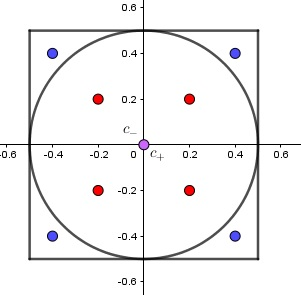
\includegraphics[width=0.5\textwidth]{pi-2d.jpg}
\centering
\caption{Círculo circunscrito no quadrado em 2 dimensões.}
\end{figure}

Dessa maneira, uma alternativa é levar as entradas para três dimensões. Isto será feito projetando o plano 2D sob uma superfície em 3D, especificamente um cone. A equação geral de um cone é dada por:
\begin{equation}
\left(\frac{x}{a}\right)^{2}+\left(\frac{y}{b}\right)^{2}=\left(\frac{z}{c}\right)^{2}
\label{hiperboloide}
. \end{equation}
Neste ponto é necessário prestar atenção em algumas condições que a Mecânica Quântica impõe.  Trabalhando com um sistema de 2 qubits, então um estado qualquer do sistema é dado por:
\begin{equation}
\left|\psi\right\rangle =\sum_{i=0}^{3}a_{i}\left|i\right\rangle 
. \end{equation}Pela condição de normalização, tem-se que $\sum_{i=0}^{3}a_{i}^{2}=1$, o que implica obviamente em que $0\leq a_{i}\leq1$. A princípio, a amplitude $a_3$ será ignorada para que seja possível focar nas outras e em um espaço de 3 dimensões. Escrevendo um conjunto de vetores ortogonais no espaço 3D e utilizando as outras três amplitudes:
\begin{equation}
\begin{split}
\left|u\right\rangle  & =\left(a_{0},0,0\right)^{T}, \\
\left|v\right\rangle & =\left(0,a_{1},0\right)^{T}, \\
\left|w\right\rangle & =\left(0,0,a_{2}\right)^{T}. \\
\end{split}
 \end{equation}
Mas, lembrando que, pela condição de normalização, para qualquer vetor escrito como uma combinação linear destes, isto é $\left|b\right\rangle=\left|u\right\rangle+\left|v\right\rangle+\left|w\right\rangle$, não é possível ter módulo maior que $1$, ou seja $\left\Vert \left|b\right\rangle \right\Vert \leq 1$. Isso implica no fato de que algumas configurações não são permitidas, por isso é necessário reduzir o tamanho do quadrado inicial, pois neste modelo, seria impossível gerar pontos que correspondessem à algumas coordenadas como por exemplo $\left(x,y\right)=\left(\pm1,\pm1\right)$ . Pode-se notar também que o valor máximo simultâneo de três coeficientes é $1/\sqrt{3}$.  Logo, de modo análogo ao que foi feito em duas dimensões, isto é, um quadrado centrado na origem, agora há um cubo de 3 dimensões também centrado na origem, e este cubo está inteiramente contido em uma esfera de raio $1$  o que respeita a condição de normalização, pois é possível apontar para qualquer ponto no interior deste quadrado com um vetor de módulo menor que $1$. Lembrando que até o momento toda discussão centrou-se em $3$ dos coeficientes. Logo, o último coeficiente é responsável por garantir a normalização do vetor de estado do sistema, isto é $a_{3}=\sqrt{1-a_{0}^{2}-a_{1}^{2}-a_{3}^{2}}$ .

Até aqui, foi garantido que as coordenadas $\left(x,y\right)$ assumam valores aceitáveis. Porém, também é necessário garantir que o mesmo também aconteça na coordenada $z$, isto é, é necessário escolher as contantes $a,b,c$ na equação do cone de modo que dado um ponto $\left(x,y\right)$ qualquer, $z$  também esteja contido na caixa, isto é $-1/\sqrt{3}\leq z\leq1/\sqrt{3}.$  Chamando de $f\left(x,y\right)$  a função responsável por projetar o plano 2D nesta superfície, então:
\begin{equation}
f\left(x,y\right)=z=c\sqrt{\left(\frac{x}{a}\right)^{2}+\left(\frac{y}{b}\right)^{2}}
. \end{equation}Dito isso, os valores escolhidos foram $\left(a,b,c\right)=\left(\sqrt{2},\sqrt{2},1\right)$ , pois assim é garantido que os pontos mais ``altos'' da superfície ainda estão contidos no cubo, isto é $f\left(\pm\frac{1}{\sqrt{3}},\pm\frac{1}{\sqrt{3}}\right)=\frac{1}{\sqrt{3}}$.  Logo:
\begin{equation}
f\left(x,y\right)=\sqrt{\frac{x^{2}+y^{2}}{2}}
\label{mapa}
. \end{equation}
Agora é possível projetar os pontos inicialmente em 2 dimensões em um espaço de 3 dimensões utilizando a função (\ref{mapa}), e, apesar dos pontos médios $\left|c_{\pm}\right\rangle $ estarem aproximadamente nas mesmas coordenadas em $x$ e $y$, deverão apresentar uma distância considerável em $z$, tornando possível a classificação correta de novos pontos.

 \begin{figure}[ht]
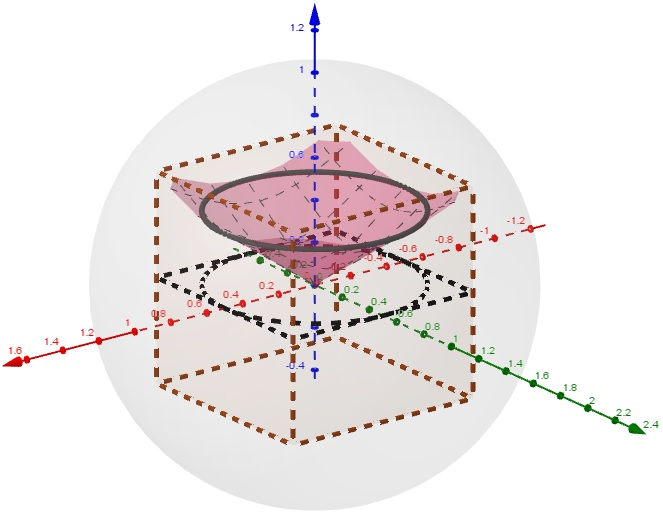
\includegraphics[width=0.75\textwidth]{pi-3d.jpg}
\centering
\caption{Esfera de raio $1$ com o quadrado de lado $1$ em seu interior e a projeção da circunferência no cone.}
\end{figure}

Porém, até agora  $a_3$ foi negligenciado. Mas o produto interno será calculado em um espaço de 4 dimensões. Pode-se dizer que a última componente da quarta dimensão é inversamente proporcional ao módulo do vetor formado pelas outras 3 componentes. Ainda que não haja recurso visual para visualizar 4 dimensões, o produto interno segue apresentando as propriedades desejas. Por exemplo, dado um vetor $\left|b\right\rangle=\left(b_{0},b_{1},b_{2},\sqrt{1-b_{0}^{2}-b_{1}^{2}-b_{2}^{2}}\right)^{T}$ qualquer, o produto interno dele com ele mesmo apresenta o máximo de semelhança:
\begin{equation}
\left\langle b|b\right\rangle =b_{0}^{2}+b_{1}^{2}+b_{2}^{2}+1-b_{0}^{2}-b_{1}^{2}-b_{2}^{2}=1
. \end{equation}
Vale destacar duas coisas: apenas a folha de cima do cone é utilizada, e os termos $x$ e $y$ aparecem sempre ao quarado na função (\ref{mapa}), ou seja $z=f\left(\pm x,\pm y\right)$. Então,  um vetor em sentido contrário no plano $x\times y$  é $\left|b_{-}\right\rangle=\left(-b_{0},-b_{1},b_{2},\sqrt{1-b_{0}^{2}-b_{1}^{2}-b_{2}^{2}}\right)^{T}$ , e o produto interno então é:
\begin{equation}
\begin{split}
\left\langle b_{-}|b\right\rangle & =-b_{0}^{2}-b_{1}^{2}+b_{2}^{2}+1-b_{0}^{2}-b_{1}^{2}-b_{2}^{2} \\
& = 2\left(-b_{0}^{2}-b_{1}^{2}\right)+1.
\end{split}
 \end{equation}
Os pontos menos semelhantes são pontos nos extremos em que $\left(x,y\right)=\pm \left(0.5,0.5\right)$, então:
\begin{equation}
\begin{split}
\left\langle b_{-}|b\right\rangle  & =2\left(-\frac{1}{4}-\frac{1}{4}\right)+1 \\
& =0.
\end{split}
\end{equation}
Resumindo, nosso método consiste em: 
\begin{itemize}
\item Definimos um quadrado de lado máximo $2/\sqrt{3}$  e centrado na origem;
\item No interior do quadrado definimos um círculo também centrado na origem;
\item Geramos pontos aleatórios em 2 dimensões no interior deste quadrado;
\item Levamos estes pontos para o espaço de \textit{Hilbert} de 4 dimensões, onde cada ponto se torna um vetor do tipo:\begin{equation}
\left|\psi\right\rangle =a_{0}\left|00\right\rangle +a_{1}\left|01\right\rangle +a_{2}\left|10\right\rangle +a_{3}\left|11\right\rangle 
. \end{equation}
\begin{itemize}
    \item Sendo os coeficientes dados por: \begin{equation}
\begin{split}
a_0 & = x,\\
a_1 & = y, \\
a _ 2 & =\sqrt{\frac{x^{2}+y^{2}}{2}},\\
a_3 & = \sqrt{1-a_{0}^{2}-a_{1}^{2}-a_{2}^{2}}.
\end{split}
\end{equation}
\end{itemize}
\item Aplicamos então o método kernel no espaço de 4 dimensões e associamos novos pontos à uma das classes binárias (dentro ou fora).
\end{itemize}

\section{Trabalhos relacionados}
Conforme mencionado anteriormente, a ideia de trabalhar com aprendizado de máquina em computadores quânticos já é bem conhecida dentro da academia, sendo assim é de se esperar a existência de outros trabalhos na área, nos quais este próprio trabalho também se baseou. 

O primeiro artigo que se destaca neste aspecto é um artigo de 2019  de Tacchino e colaboradores. Neste artigo, foi proposto e implementado um modelo híbrido de treinamento para um perceptron binário, além disso também são propostos 2 algoritmos (bloco de mudança de sinal de HSGS) para o cálculo do produto interno no computador quântico e é sugerida a possibilidade da construção de um modelo contínuo utilizando as fases dos números complexos envolvidos \cite{Italiano}.   Desta forma, este artigo serviu como base para a implementação do modelo híbrido de treinamento para o perceptron quântico, assim como inspiração para a elaboração do modelo contínuo.

Outro artigo mais recente, datado de 2019  é de Havlíček e colaboradores \cite{havlivcek2019supervised}. Diferente do artigo anterior, que é baseado na proposta e implementação de rede neurais, este propõe e implementa um  modelo baseado em método kernel, também baseado em um esquema de treinamento híbrido. Assim, esta pesquisa serviu como inspiração para a escolha do terceiro modelo proposto. Porém, o modelo original apresentado pelo artigo se aproxima do estado da arte e requer elevado grau de domínio da área, o que exigiria um tempo de estudo além do disponível para a elaboração do presente trabalho. Por esta razão, optou-se por implementar um modelo simplificado como introdução ao método kernel em computadores quânticos.

Em 2020, Gabor e colaboradores publicaram um interessante artigo sobre a inteligência artificial quântica, no qual é discutido o estado da arte e os principais desafios atuais da área \cite{gabor2020holy}. O autores classificam como o ``Santo Graal da IA Quântica'' o problema do \textit{feedback}, isto é, substituir os \textit{loops} que usualmente ocorrem durante o treinamento de diferentes modelos de inteligência artificial por um algoritmo inteiramente quântico. Porém, ao reconhecer a necessidade de processar uma quantidade relativamente grande de dados de treinamento, pondera-se sobre a possibilidade de que isto pode impedir que o \textit{loop} de treinamento seja inteiramente removido. Então é proposto que a chave para um maior desenvolvimento da IAQ (Inteligência Artificial Quântica) está na combinação e hibridização de vários algoritmos e técnicas, isto é, utilizar abordagens híbridas que permitam a construção de etapas de pré/pós processamento clássico.

Em outro artigo também de 2020, Lloyd e colaboradores propõem um modelo híbrido utilizando o método kernel através de uma estratégia que chamam de métrica quântica de aprendizagem \cite{lloyd2020quantum}. Esta estratégia poderia ser implementada em plataformas de computação quântica de médio prazo, apesar de incluir a representação de dados clássicos como estados quânticos no espaço de Hilbert via uma função denominada mapa de recursos quânticos (\textit{quantum feature map}), processo conhecido como incorporação quântica (\textit{quantum embedding}). Este é um processo que em geral não pode ser reproduzido em computadores clássicos, portanto deixa em aberto a possibilidade de uma vantagem quântica. É interessante lembrar outro artigo mais antigo no qual Lloyd fez parte, datado de 2014 \cite{Rebentrost_2014}. Foi um estudo liderado por Rebentrost que foi apoiado dentre outros pela DARPA (Agência de Projetos de Pesquisa Avançada de Defesa dos EUA) e pelo Laboratório de Inteligência Artificial Google-NASA. Neste artigo é proposto um modelo também baseado no método kernel, considerado um algoritmo quântico para trabalhar com grandes quantidades de dados (\textit{big data}), e tem como característica de destaque maior segurança na privacidade dos dados envolvidos no processo quando comparado com alternativas clássicas, além de um ganho de velocidade no processamento.

Winci e colaboradores publicaram um artigo também em 2020 no qual destacam que o desenvolvimento de modelos híbridos quânticos-clássicos são o estado da arte da área. Neste trabalho foi proposto também um modelo híbrido de redes neurais no qual sugerem que pode ser o caminho em direção de alcançar uma vantagem quântica, isto é, através do seu modelo o computador quântico seria capaz de resolver problemas no qual a computação clássica se mostrou lenta e ineficiente \cite{Winci_2020}. Do mesmo ano e também discutindo um possível caminho para a vantagem quântica, temos um artigo do Coyle colaboradores \cite{vantagem}.

Porém, antes de discutir qual seria este caminho, este trabalho nos apresenta a definição do que seria a chamada supremacia quântica: a capacidade de dispositivos quânticos fornecerem soluções eficientes para problemas que não podem ser resolvidos em um tempo polinomial por meios clássicos. De acordo com Coyle, a demonstração desta capacidade  seria uma demonstração da chamada supremacia quântica. Neste artigo, além de propor um modelo híbrido de aprendizado de máquina, os autores também propõem a existência de uma chamada supremacia quântica de aprendizagem, isto é, uma vantagem de dispositivos e modelos quânticos sobre suas alternativas clássicas dentro do contexto de aprendizagem de máquina. Esta é uma proposta baseada na possibilidade de que existam algumas classes de distribuições que não podem ser eficientemente aprendidas por computadores clássicos, mas que podem ser aprendidas em dispositivos quânticos.

Por fim, Zhang e Ni, também em 2020, publicaram um artigo no qual discutem os avanços recentes no aprendizado de máquina quântico, nos dando uma visão geral do estado da arte. Sendo um artigo de revisão, ele possui uma estrutura bastante interessante, inclusive para um primeiro contato com a área, pois nos seus dois primeiros tópicos apresenta alguns conceitos de computação quântica para aqueles que estão familiarizados apenas com a mecânica quântica, além de discutir alguns algoritmos já conhecidos da computação quântica, como o Algoritmo de Grover e o HHL \cite{ultimo}. Na sequência,  discute a aplicação de alguns algoritmos para o aprendizado de máquina quântico. É interessante aqui destacar o Support Vector Machine (SVM), que é um método kernel e aparece repetidamente em diversos artigos e as redes neurais quânticas, que foram os dois modelos no qual este TCC se baseou. Além disso, é discutido  sobre o algoritmo de clusterização conhecido como K-means quântico e alguns algoritmos quânticos de redução de dimensionalidade (QPCA e QLDA).

Concluindo, os autores nos lembram que apesar de muitos pesquisadores terem demonstrado um ganho no tempo de processamento nas versões quânticas dos algoritmos de máquina de aprendizado em comparação com suas contra-partidas clássicas, ainda há alguns problemas na área. Como por exemplo a entrada e saída de dados.


\chapter{Resultados}

\section{Modelagem do circuito quântico}

Dado um vetor de entrada de dimensão $m$, o mesmo deve ser codificado usando $m$  coeficientes para definir uma função de onda geral $\left|\psi_{i}\right\rangle $. Na prática, dados vetores de entrada e pesos arbitrários temos:
\begin{equation}\overrightarrow{i}=\left(\begin{array}{c}
i_{0}\\
i_{1}\\
\vdots\\
i_{m-1}
\end{array}\right),\qquad\overrightarrow{w}=\left(\begin{array}{c}
w_{0}\\
w_{1}\\
\vdots\\
w_{m-1}
\end{array}\right). \end{equation}
Dessa forma, pode-se definir os seguintes estados quânticos:
\begin{equation}\left|\psi_{i}\right\rangle =\frac{1}{\sqrt{m}}\sum_{j=0}^{m-1}i_{j}\left|j\right\rangle, \qquad\left|\psi_{w}\right\rangle =\frac{1}{\sqrt{m}}\sum_{j=0}^{m-1}w_{j}\left|j\right\rangle  . \end{equation}
Os estados $\left|j\right\rangle =\in\left\{ \left|00\ldots00\right\rangle ,\left|00\ldots01\right\rangle ,\dots,\left|11\ldots11\right\rangle \right\} $ formam a base computacional do processador quântico, no qual vamos identificar cada estado por inteiros decimais que são formados a partir da respectiva string binária $\left|j\right\rangle \in\left\{ \left|0\right\rangle ,\left|1\right\rangle ,\dots,\left|m-1\right\rangle \right\} $. Evidentemente se há $N$ qubits no registrador, então haverá  $m=2^{N}$ estados. Dessa maneira como motivação inicial, pode-se pensar em ter como objetivo  que o circuito quântico seja capaz de efetuar o seguinte cálculo:
\begin{equation}
\left\langle \psi_{i},\psi_{w}\right\rangle =\frac{\overrightarrow{w}\cdot\overrightarrow{v}}{m} 
\label{prodin}
. \end{equation}
Assumindo que os qubits são inicializados em $\left|00\dots00\right\rangle \equiv\left|0\right\rangle ^{\otimes N}$, o primeiro passo é preparar o estado $\left|\psi_{i}\right\rangle $ através de uma transformação unitária $U_{i}$ com os valores de entrada em $\overrightarrow{i}$ codificados. Ou seja, o operador de entrada deve ser capaz de realizar a seguinte transformação:
\begin{equation}U_{i}\left|0\right\rangle ^{\otimes N}=\left|\psi_{i}\right\rangle . \end{equation}
Em princípio, qualquer matriz $m \times m$ unitária com $\overrightarrow{i}$ na primeira coluna serve. O  próximo passo é realizar uma  transformação unitária $U_{w}$ com os valores do peso  $\overrightarrow{w}$ codificados  de maneira que leve o resultado do produto interno da equação (\ref{prodin}) ao último coeficiente da base computacional. Explícitamente, queremos o seguinte comportamento:
\begin{equation}
\begin{split}
U_{w}\left|\psi_{i}\right\rangle & =\left[\frac{1}{\sqrt{m}}\left(\begin{array}{cccc}
A_{11} & A_{21} & \cdots & A_{1\left(m-1\right)}\\
A_{12} & A_{22} & \cdots & A_{2\left(m-1\right)}\\
\vdots & \vdots & \ddots & \vdots\\
\overline{w_{0}} & \overline{w_{1}} & \ldots & \overline{w_{m-1}}
\end{array}\right)\right]\left[\left(\begin{array}{c}
i_{0}\\
i_{1}\\
\vdots\\
i_{m-1}
\end{array}\right)\frac{1}{\sqrt{m}}\right] \\
& =\left(\begin{array}{c}
C_{1}\\
C_{2}\\
\vdots\\
\sum_{j=0}^{m-1}\overline{w_{j}}i_{j}
\end{array}\right)\frac{1}{m}.
\end{split}
\end{equation}
Onde $A_{ij}$  e $C_{i}$ denotam coeficientes irrelevantes para nosso propósito. Semelhante ao caso do operador de entrada,  em princípio qualquer matriz $m \times m$ unitária com o conjugado de $\overrightarrow{w}$ na última linha serve. Porém, para justificar alguns algoritmos propostos nas próximas seções para construção do circuito mais algumas demonstrações matemáticas  se tornam relevantes. Em especial, o operador $U_{w}$  deve ser capaz de realizar a seguinte transformação:
\begin{equation}U_{w}\left|\psi_{w}\right\rangle =\left|1\right\rangle ^{\otimes N}=\left|m-1\right\rangle. \end{equation}
Onde $\left|m-1\right\rangle$  corresponde ao último estado da base computacional. Após a aplicação de ambos operadores, o estado final  pode ser decomposto na base computacional, isto é:
\begin{equation}U_{w}U_{i}\left|0\right\rangle ^{\otimes N}=U_{w}\left|\psi_{i}\right\rangle =\sum_{j=0}^{m-1}c_{j}\left|j\right\rangle . \end{equation}
Denotando o estado final como $\left|\phi_{i,w}\right\rangle \equiv U_{w}U_{i}\left|0\right\rangle  ^{\otimes N}$ , e como $U_{w}$ é um operador unitário, então o produto interno entre $\left|\psi_{i}\right\rangle $ e $\left|\psi_{w}\right\rangle $ pode ser escrito como:
\begin{equation}
\begin{split}
\left\langle \psi_{w} | \psi_{i} \right\rangle & =\left\langle \psi_{w} \left| U_{w}^{\dagger}U_{w} \right| \psi_{i} \right\rangle \\
&  =\left\langle m-1|\phi_{i,w}\right\rangle \\
& =\sum_{j}^{m-1}c_{j}\left\langle m-1|j\right\rangle \\
& = c_{m-1}.
\end{split}
\end{equation}
Torna-se evidente que o resultado que nos interessa é o coeficiente $c_{m-1} $ do estado final do  processador após ambas transformações unitárias serem aplicadas. Ainda, podemos usar um qubit auxiliar $a$  inicialmente no estado $\left|0\right\rangle $  e um operador NOT multi-controlado entre os $N$ qubits que codificam a informação e o alvo $a$. Isto leva a:
\begin{equation}\left|\phi_{i,w}\right\rangle \left|0\right\rangle \rightarrow\sum_{j=0}^{m-2}c_{j}\left|j\right\rangle \left|0\right\rangle _{a}+c_{m-1}\left|m-1\right\rangle \left|1\right\rangle _{a}. \end{equation}
Desse modo é necessário medir apenas a probabilidade do qubit auxiliar $a$ estar no estado $\left|1\right\rangle$. Concluindo, a saída final do circuito quântico que será medida é  $\left|C_{m-1}\right|^{2}$. Então o valor a ser medido após a aplicação do algoritmo é:
\begin{equation}\left|\left\langle \psi_{w}|\psi_{i}\right\rangle \right|^{2}=\frac{\left|\overrightarrow{w}\cdot\overrightarrow{v}\right|^{2}}{m^{2}}. \end{equation} 
Um esquema geral do algoritmo responsável por este cálculo está ilustrado na figura \ref{UM}. 

\begin{figure}[ht]
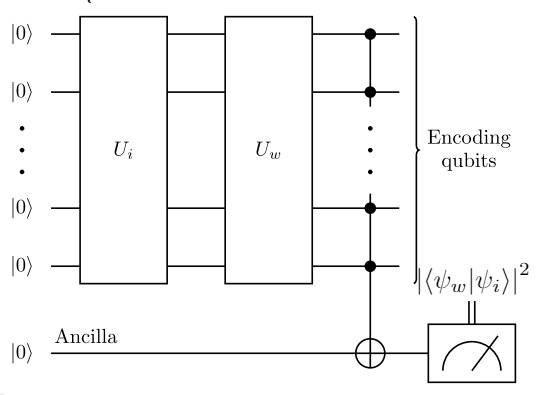
\includegraphics[width=0.75\textwidth]{img1.jpg}
\centering
\caption{Esquema geral do algoritmo quântico responsável pelo produto interno.}
\label{UM}
\end{figure}

\section{Especificação das transformações unitárias}

O próximos dois algoritmos foram desenhados pensando nas redes neurais, isto é, trabalham apenas com a variação da fase dos números complexos. Em ambos os modelos, as variáveis de entradas e pesos estão presentes nas fases dos números complexos, isto é $i_{j},w_{j}\in\left\{ e^{i\theta}\right\} $, com $0\leq \theta \leq 2 \pi $, e a informação pode ser codificada em uma superposição uniforme de toda base computacional, já que alterar a fase do número complexo não altera seu módulo. Também podemos lembrar que o caso binário do perceptron se torna apenas um caso especial dos valores contínuos do sigmoide, para valores extremos de $\theta$.

\subsection{Bloco de rotação de fase }

Como primeira etapa, vamos definir um bloco de rotação de fase $B_{N,j}\left(\lambda\right)$ como uma  transformação unitária atuando na base computacional de $N$ qubits da seguinte forma:
\begin{equation}B_{N,j} \left( \lambda \right) \left| j' \right\rangle = \left\{ \begin{array}{ccc} e^{i\lambda} \left| j' \right\rangle & ,\text{se} & j=j' \\ \left| j' \right\rangle & , \text{se} & j\neq j' \end{array} \right. . \end{equation}
Podemos implementar uma família de blocos de  rotação de fase para $N$ qubits usando uma rotação de fase multi-controlada $C_{u1}\left(\lambda\right)$ em combinação com operadores NOT em qubits unitários:
\begin{equation}B_{N,j}\left(\lambda\right)=O_{j}\left[C_{u1}\left(\lambda\right)\right]O_{j}. \end{equation}
Onde $ O_{j}=\otimes_{l=0}^{N}\left(NOT_{l}\right)^{1-j_{l}}$  é a expressão responsável por levar o coeficiente alvo para o estado $\left|m-1\right\rangle $ da base computacional. Então é possível aplicar a rotação de fase multi-controlada $C_{u1}\left(\lambda\right)$  tendo como alvo o qubit $N$. Desta maneira irá alterar a fase somente do coeficiente alvo, e então $O_j$ pode ser novamente  utilizado  para trazer o coeficiente a seu estado original. $NOT_{l}$ significa que aplicamos o operador $NOT$ no \textit{l-ésimo} qubit, e $j_{l}=0$ se o l-ésimo qubit está no estado $\left|0\right\rangle $ ($j_{l}=1$ se o estado for $\left|1\right\rangle $). É importante notar que $j_{l}=0$ implica em de fato aplicarmos a operação $NOT$  no qubit $l$, mas $j_{l}=1$ significa que usamos o operador identidade para manter o \textit{l-ésimo} qubit inalterado. Uma característica importante  do bloco de rotação de fase é manter inalterado todos os coeficientes que não sejam o alvo. 

Com o bloco de rotação de fase definido, pode-se resumir a sequência completa da implementação de $U_{i}$, lembrando da definição do operador de entrada ($U_{i}\left|0\right\rangle ^{\otimes N}=\left|\psi_{i}\right\rangle $) da seguinte forma:
\begin{itemize}
\item Partindo  do registrador inicializado em $\left|0\right\rangle ^{\otimes N}$, aplica-se operadores de Hadamard em cada qubit para criar um estado de total sobreposição entre todos os elementos da base computacional: $\left|0\right\rangle ^{\otimes N}\stackrel{H^{\otimes N}}{\rightarrow}\frac{1}{\sqrt{m}}\sum_{j=0}^{m-1}\left|j\right\rangle \equiv\left|\psi_{0}\right\rangle  $;
\end{itemize}
\begin{itemize}
\item Então é necessário apenas aplicar os blocos de rotação de fase nos coeficientes que forem necessários.
\begin{itemize}
\item Como o bloco de rotação de fase mantém os outros coeficientes inalterados, deste modo a ordem de aplicação torna-se irrelevante.
\end{itemize}
\end{itemize}

O operador $U_{w}$ é definido de maneira similar mas em ordem inversa. Levando em conta como é definido ($U_{w}\left|\psi_{w}\right\rangle =\left|1\right\rangle ^{\otimes N}=\left|m-1\right\rangle$), temos então:
\begin{itemize}
\item Aplica-se os blocos de mudança de fase com negativo da fase do peso de forma que leve o estado computacional atual ao estado de sobreposição:  $\left|\psi_{w}\right\rangle \stackrel{B_{N,j}\left(- \lambda\right)}{\rightarrow}\left|\psi_{0}\right\rangle $;
\item Com o operador de Hadamard  aplicado em cada qubit, o estado final do sistema se torna o estado inicial do processador, isto é: $\left|\psi_{0}\right\rangle \stackrel{H^{\otimes N}}{\rightarrow}\left|0\right\rangle ^{\otimes N}$;
\item Então, com um operador NOT aplicado em cada qubit, o sistema vai para o estado desejado: $\left|0\right\rangle ^{\otimes N}\stackrel{NOT^{\otimes N}}{\rightarrow}\left|1\right\rangle ^{\otimes N}$.
\end{itemize}

É interessante aqui destacar que o complexo conjugado de um número complexo qualquer   $z=e^{i\lambda}$  equivale a outro número complexo de mesmo módulo e com uma fase equivalente ao seu negativo $\overline{z}=e^{-i\lambda}$. Portanto aplicar uma rotação de fase a $z$ equivalente ao negativo da sua própria fase equivale a multiplicar $z$ pelo seu conjugado: $\overline{z}z=e^{-i\lambda}e^{i\lambda}=1$. De forma que estamos construindo um operador $U_{w}$ que a última linha é o conjugado de $\overrightarrow{w}$, como desejamos.

\begin{figure}[ht]
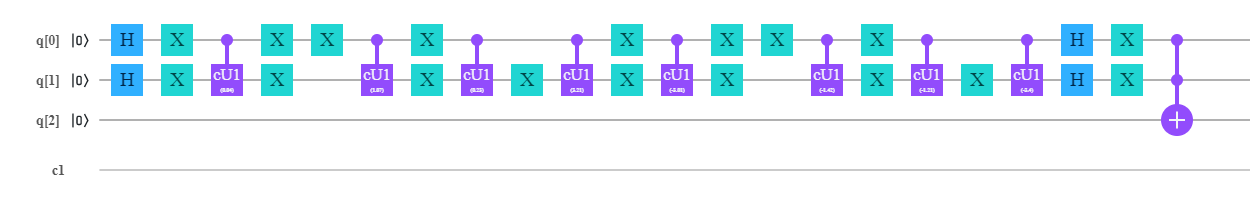
\includegraphics[width=1\textwidth]{img2.png}
\centering
\caption{Exemplo de circuito utilizando o algoritmo dos blocos de rotação de fase.}
\label{DOIS}
\end{figure}
Um exemplo de circuito construído utilizando os blocos de rotação de fase está ilustrado na figura \ref{DOIS}.

\subsection{HSGS}

Uma solução que espera-se ser mais eficiente para variar a fase dos números complexos é o algoritmo HSGS. Este algoritmo espera-se ser capaz de reduzir os recursos quânticos necessários em comparação com o método dos blocos de rotação de fase apresentado anteriormente. Isto ocorre, principalmente, porque ainda que continue apresentando um custo exponencial, o algoritmo HSGS otimiza o número de operadores multi-controlados necessários \cite{Italiano}.

Olhando primeiro a construção do operador $U_{i}$ ,  tendo então um estado de sobreposição total $H^{\otimes N}$,  o primeiro passo é aplicar o operador $u_{1}$ (rotação de fase) no coeficiente dos estados que tenham apenas $p=1$ bit no estado $\left|1\right\rangle $ (e.g. na forma $\left|0\dots010\dots0\right\rangle $) , em seguida aplicamos as correções necessárias no estados que apresentam $p=2$  usando uma rotação de fase multi-controlada $c^{p}u_{1}$ com os qubits já alterados como qubits de controle. Então prosseguimos até $p=N$, quando restará somente o estado $\left|0\right\rangle ^{\otimes N}$ inalterado. Se necessário, podemos utilizar   $X^{\otimes N}$   e  $c^{N}u_{1}$  para alterá-lo.

Sobre o operador peso, de forma análoga ao que ocorre com os blocos de rotação de fase, é necessário fazer o processo no sentido inverso, com o objetivo inicial de levar do estado peso $\left| \psi_{w} \right\rangle $  para um estado de sobreposição equilibrada, e então aplicar de forma paralela os operadores  $H^{\otimes N}$ e $NOT^{\otimes N}$. A figura \ref{TRES} ilustra a construção de um circuito utilizando este algoritmo.
\begin{figure}[ht]
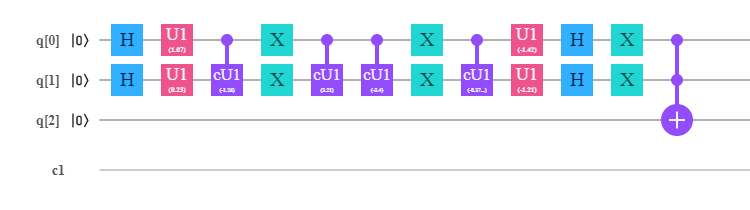
\includegraphics[width=1\textwidth]{img3.png}
\centering
\caption{Exemplo de circuito utilizando o algoritmo HSGS.}
\label{TRES}
\end{figure}
\subsection{Método kernel}

Vamos usar um modelo inspirado nos blocos de rotação de fase, ou seja, vamos construir blocos de variação de módulo. Porém, como precisamos manter a normalização do vetor, vamos sempre alterar em pares, vamos optar por alterar usando o último coeficiente como controle, e vamos nos preocupar com a variação do módulo dos outros coeficientes. Usando a seguinte sequência de operações, podemos variar apenas o primeiro e último coeficiente: $M_1=\left(X\otimes\mathbb{I}\right).cX_{0}.cX_{1}.cu_{3}.cX_{1}.cX_{0}.\left(X\otimes\mathbb{I}\right)$, onde $cX_i$ in dica que é um $X$ controlado usando o qubit $i$ como de controle e $cu_3$  é a versão controlada do operador $u_3$, isto é, a rotação de um único qubit com os 3 ângulos de Euler. Esta sequência de operações resulta na seguinte matriz:

\begin{equation}
M_1=\left[\begin{array}{cccc}
\cos\left(\frac{a}{2}\right) & 0 & 0 & -\sin\left(\frac{a}{2}\right)\\
0 & 1 & 0 & 0\\
0 & 0 & 1 & 0\\
\sin\left(\frac{a}{2}\right) & 0 & 0 & \cos\left(\frac{a}{2}\right)
\end{array}\right]
. \end{equation}
Para o segundo coeficiente podemos usar apenas o operador $cu_3.$ Sendo $\theta=\lambda=0$ temos:
\begin{equation}
M_2=\left[\begin{array}{cccc}
1 & 0 & 0 & 0\\
0 & \cos\left(\frac{b}{2}\right) & 0 & -\sin\left(\frac{b}{2}\right)\\
0 & 0 & 1 & 0\\
0 & \sin\left(\frac{b}{2}\right) & 0 & \cos\left(\frac{b}{2}\right)
\end{array}\right]
. \end{equation}
E, por fim, para o terceiro coeficiente podemos usar: $M_3=cX_{1}.cX_{0}.cX_{1}.cu_{3}.cX_{1}.cX_{0}.cX_{1}$:
\begin{equation}
M_3=\left[\begin{array}{cccc}
1 & 0 & 0 & 0\\
0 & 1 & 0 & 0\\
0 & 0 & \cos\left(\frac{c}{2}\right) & -\sin\left(\frac{c}{2}\right)\\
0 & 0 & \sin\left(\frac{c}{2}\right) & \cos\left(\frac{c}{2}\right)
\end{array}\right]
. \end{equation}
Cada uma dessas matrizes altera a amplitude de apenas um dos coeficientes. Quando aplicamos as três, temos na seguinte sequência $U_a=M_3.M_2.M_1.$
\begin{equation}
U_a=\left[\begin{array}{cccc}
\cos\left(\frac{a}{2}\right) & 0 & 0 & -\sin\left(\frac{a}{2}\right)\\
-\sin\left(\frac{a}{2}\right)\sin\left(\frac{b}{2}\right) & \cos\left(\frac{b}{2}\right) & 0 & -\cos\left(\frac{a}{2}\right)\sin\left(\frac{b}{2}\right)\\
-\sin\left(\frac{a}{2}\right)\cos\left(\frac{b}{2}\right)\sin\left(\frac{c}{2}\right) & -\sin\left(\frac{b}{2}\right)\sin\left(\frac{c}{2}\right) & \cos\left(\frac{c}{2}\right) & -\cos\left(\frac{a}{2}\right)\cos\left(\frac{b}{2}\right)\sin\left(\frac{c}{2}\right)\\
\sin\left(\frac{a}{2}\right)\cos\left(\frac{b}{2}\right)\cos\left(\frac{c}{2}\right) & \sin\left(\frac{b}{2}\right)\cos\left(\frac{c}{2}\right) & \sin\left(\frac{c}{2}\right) & \cos\left(\frac{a}{2}\right)\cos\left(\frac{b}{2}\right)\cos\left(\frac{c}{2}\right)
\end{array}\right]
\label{matrao}
. \end{equation}
Aplicando no estado inicial $\left|\psi_{0}\right\rangle =\left[\begin{array}{cccc}
1 & 0 & 0 & 0\end{array}\right]^{T}$ temos:
\begin{equation}
\left|a\right\rangle =\left[\begin{array}{c}
\cos\left(\frac{a}{2}\right)\\
-\sin\left(\frac{a}{2}\right)\sin\left(\frac{b}{2}\right)\\
-\sin\left(\frac{a}{2}\right)\cos\left(\frac{b}{2}\right)\sin\left(\frac{c}{2}\right)\\
\sin\left(\frac{a}{2}\right)\cos\left(\frac{b}{2}\right)\cos\left(\frac{c}{2}\right)
\end{array}\right]=\left[\begin{array}{c}
a_{0}\\
a_{1}\\
a_{2}\\
a_{3}
\end{array}\right]
. \end{equation}Então, sabendo os coeficientes $a_i$ do vetor $\left|a\right\rangle $,  podemos obter os ângulos através das seguintes relações:
\begin{itemize}
\item $a=2\arccos\left(a_{0}\right)$,
\item $b=2\arcsin\left(-\frac{a_{1}}{\sin\left(a/2\right)}\right)$,
\item $c=2\arccos\left(-\frac{a_{2}}{\sin\left(a/2\right)\cos\left(b/2\right)}\right)$.
\end{itemize}
Se olharmos para a equação (\ref{matrao}), a última linha também já pode ser utilizada como o vetor $\left|b\right\rangle $. Então, se aplicarmos novamente a mesma sequência de operações, mas agora com os seguintes ângulos:
\begin{itemize}
\item $c=2\arcsin\left(b_{2}\right)$,
\item $b=2\arcsin\left(\frac{b_{1}}{\cos\left(c/2\right)}\right)$,
\item $a=2\arcsin\left(\frac{a_{0}}{\cos\left(b/2\right)\cos\left(c/2\right)}\right)$.
\end{itemize}
Vamos ter:
\begin{equation}
\left|b\right\rangle =\left[\begin{array}{c}
\sin\left(\frac{a}{2}\right)\cos\left(\frac{b}{2}\right)\cos\left(\frac{c}{2}\right)\\
\sin\left(\frac{b}{2}\right)\cos\left(\frac{c}{2}\right)\\
\sin\left(\frac{c}{2}\right)\\
\cos\left(\frac{a}{2}\right)\cos\left(\frac{b}{2}\right)\cos\left(\frac{c}{2}\right)
\end{array}\right]=\left[\begin{array}{c}
b_{0}\\
b_{1}\\
b_{2}\\
b_{3}
\end{array}\right]
. \end{equation}
E aplicando a sequência de operadores $U_b\cdot A_a$ no estado inicial, tendo que a primeira coluna de $U_a$ é $\left|a\right\rangle $ e a última linha de $U_b$ é $\left\langle b\right|$:
\begin{equation}
\begin{split}
\left|\psi\right\rangle & =U_{b}\cdot U_{a}\left|\psi_{0}\right\rangle \\
&= \left[\begin{array}{cccc}
A_{11} & A_{12} & A_{13} & A_{14}\\
A_{21} & A_{22} & A_{23} & A_{24}\\
A_{32} & A_{32} & A_{33} & A_{34}\\
b_{0} & b_{1} & b_{2} & b_{3}
\end{array}\right]\left[\begin{array}{cccc}
a_{0} & A_{12} & A_{13} & A_{14}\\
a_{1} & A_{22} & A_{23} & A_{24}\\
a_{2} & A_{32} & A_{33} & A_{34}\\
a_{3} & A_{42} & A_{43} & A_{44}
\end{array}\right]\left[\begin{array}{c}
1\\
0\\
0\\
0
\end{array}\right] \\
& = \left[\begin{array}{cccc}
 A_{11} & A_{12} & A_{13} & A_{14}\\
A_{21} & A_{22} & A_{23} & A_{24}\\
A_{32} & A_{32} & A_{33} & A_{34}\\
b_{0} & b_{1} & b_{2} & b_{3}
\end{array}\right]\left[\begin{array}{c}
a_{0}\\
a_{1}\\
a_{2}\\
a_{3}
\end{array}\right].
\end{split}
 \end{equation}
Podemos notar que aqui temos $\left|\psi\right\rangle =U_{b}\left|a\right\rangle $. Prosseguindo temos:
\begin{equation}
\left|\psi\right\rangle =\left[\begin{array}{cccc}
c_{0} & c_{1} & c_{2} & \sum_{i}^{3}a_{i}b_{i}\end{array}\right]^{T}
. \end{equation}
Então o último termo de nosso estado final é $c_{3}=\left\langle b|a\right\rangle $, como queríamos. Lembrando que o valor medido será $\left|c_{3}\right|^2=\left|\left\langle b|a\right\rangle \right|^{2}$.  Porém, antes de concluirmos precisamos prestar atenção em algumas coisas. Primeiro que a ordem de aplicação dos operadores $M_i$ não é independente, e segundo que se olharmos o conjunto de equações que utilizamos para calcular os ângulos $\theta_i$ dos operadores $M_i$, podemos encontrar alguns problemas. Por exemplo, no conjunto de equações que obtemos para o operador $U_a$, temos que $-\sin\left(\frac{a}{2}\right)\sin\left(\frac{b}{2}\right)=a_{1}$  mas se $\left|\sin\left(\frac{a}{2}\right)\right|<a_{1}$  então $\left|\frac{a_{1}}{\sin\left(a/2\right)}\right|>1$ , o que leva à conclusão de que $\sin\left(\frac{b}{2}\right)>1$. Para evitar esse tipo de problema, devemos aplicar diferentes sequências de operações para situações diferentes. Para o vetor $\left|a\right\rangle $ temos simplesmente que para o caso em que $\theta_i \leq \theta_j \leq \theta_k$   vamos aplicar $M_k \cdot M_j \cdot M_i  \cdot \left(X\otimes X\right)$. Para o vetor $\left|b\right\rangle $ tendo a mesma sequência $\theta_i \leq \theta_j \leq \theta_k$, de modo análogo aos casos anteriores, utilizamos a ordem inversa, isto é: $M_i \cdot M_j \cdot M_k  $, lembrando que os ângulos $a,b,c$ devem ser também recalculados caso a caso.

\section{Resultados numéricos  e discussão}

Todos algoritmos foram implementados em Python utilizando a biblioteca NumPy (\url{https://numpy.org/}) para cálculos analíticos e o kit de desenvolvimento Qiskit para Python (\url{https://qiskit.org/}), que fornece não só simuladores quanto acesso a dispositivos reais na nuvem da IBM Quantum Experience  (\url{https://quantum-computing.ibm.com/}). Todos os testes em simuladores e a versão quântica do perceptron foi executada a partir do recurso de computação em nuvem disponibilizado pelo Google, chamado Google Colab (\url{https://colab.research.google.com/}). Através desta plataforma o Google disponibiliza um processadores Intel(R) Xeon(R) CPU @ 2.30GHz com 2 núcleos e 12GB de memória RAM. Neste ambiente também foi utilizado a versão 0.16.1 do Qiskit, no qual possui a seguinte versão de seus módulos:
\begin{itemize}
    \item qiskit-aer: 0.7.2,
    \item qiskit-aqua: 0.8.1,
    \item qiskit-ibmq-provider: 0.11.1,
    \item qiskit-ignis: 0.5.1,
    \item qiskit-terra: '0.16.1.
\end{itemize}

O ambiente disponibilizado pelo Google tem sua conexão encerrada após 12h de duração. Dessa forma para executar a versão quântica dos modelos sigmoide e kernel foi necessário utilizar um computador pessoal para manter a execução por vários dias. Sendo assim, estes modelos foram executados a partir de um computador com processador Intel(R) Core(TM) i5-6400 CPU @ 2.70GHz de 4 núcleos e 8Gb de memória RAM. Por sua vez, neste computador foi utilizada o qiskit versão 0.19.6 com a seguinte versão de seus módulos:

\begin{itemize}
    \item qiskit-terra: 0.14.2, 
    \item qiskit-aer: 0.5.2, 
    \item qiskit-ignis: 0.3.3, 
    \item qiskit-ibmq-provider: 0.7.2, 
    \item qiskit-aqua: 0.7.3.
\end{itemize}

\subsection{Produto interno}

Para comparar o resultado entre os algoritmos propostos (blocos de rotação e HSGS) , foi utilizada a seguinte medida quantitativa  de discrepância média proposta por Tacchino e colaboradores \cite{Italiano}:

\begin{equation}D=\frac{\sum_{k=1}^{n}\left|O_{IBM}^{\left(k\right)}-O_{ideal}^{\left(k\right)}\right|}{n},\end{equation}
onde para $n$ saídas calculadas, fazemos a diferença entre a saída ideal ($O_{ideal}^{\left(k\right)}$  ), calculada classicamente, e a saída dos dispositivos reais da IBM ($O_{IBM}^{\left(k\right)}$), obtidas através do Qiskit.  Devido a limitações impostas no uso do hardware da IBM, como por exemplo filas de utilização, limitamos ao caso com $N=2$  qubits.

Para comparação, primeiro foi reproduzido o modelo binário, onde ao invés de utilizarmos o operador $u_{1}$ responsável por executar uma variação $\theta$ genérica na fase, é utilizado então um operador $Z$ que executa simplesmente uma mudança de sinal. Com $N=2$ qubits,  é possível construir $2^{4}=16$ vetores unitários e binários diferentes que geram $n=2^{2^{4}}=256$ produtos distintos possíveis entre si. Foi calculada então a saída esperada analiticamente e a saída obtida através do dispositivo quântico. Neste trabalho, o cálculo foi reproduzido 5 vezes em 3 dispositivos quânticos diferentes, com preferência para o \textit{`ibmq\_vigo'} devido a ter apresentado os melhores resultados. O resultado pode ser visto na Tabela \ref{tabela1}.

\begin{table}[h!]
\caption{Discrepância para o produto interno entre vetores binários}
\label{tabela1}
\centering
\resizebox{\textwidth}{!}{%
\begin{tabular}{l|l|l|}
\hline
\multicolumn{1}{|l|}{\textbf{Dispositivo}} & \textbf{Bloco de rotação} & \textbf{HSGS}         \\ \hline
\multicolumn{1}{|l|}{ibmq\_5\_yorktown}    & 0.22016143798828125       & 0.22871780395507812   \\ \hline
\multicolumn{1}{|l|}{ibmq\_valencia} & 0.1013946533203125 & 0.1109771728515625  \\ \hline
\multicolumn{1}{|l|}{ibmq\_vigo} & 0.09790420532226562 & 0.08685302734375   \\ \hline
\multicolumn{1}{|l|}{ibmq\_vigo} & 0.09388351440429688 & 0.08945083618164062   \\ \hline
\multicolumn{1}{|l|}{ibmq\_vigo} & 0.10137939453125 & 0.0917205810546875   \\ \hline
\end{tabular}%
}
\end{table}

Podemos notar que não parece haver uma diferença significativa nos resultados. A diferença média entre os resultados dos algoritmos foi de $\left(1.40\pm8.83\right)\times10^{-3}$, isto é, o desvio padrão foi maior que a própria média em módulo. O que indica que podemos esperar que dependendo da execução, um algoritmo ou outro pode se sair um pouco melhor. Este resultado contraria o esperado pelo que consta na literatura. Maior investigação é necessária, mas uma hipótese a ser levantada é que este resultado pode ser decorrente da estrutura dos processadores utilizados. HSGS possibilita uma vantagem significativa em processadores que não possuem operações de múltiplos qubits disponíveis nativamente \cite{Italiano}. Porém como mencionado anteriormente, maior investigação é necessária.

A próxima etapa foi trabalhar com os vetores de valores contínuos. Devido a limitações de tempo e a possibilidade de construção de infinitos vetores contínuos, foi optado por trabalhar com apenas $8$ vetores de valores contínuos gerados aleatoriamente. De maneira que torna-se possível combinar os $8$ vetores para calcularem  $n=8^{2}=64$ produtos internos distintos entre si. O resultado  é apresentado na Tabela \ref{tabela2}.

\begin{table}[h!]
\caption{Discrepância para o produto interno entre vetores contínuos}
\label{tabela2}
\centering
\resizebox{\textwidth}{!}{%
\begin{tabular}{l|l|l|}
\hline
\multicolumn{1}{|l|}{\textbf{Dispositivo}} & \textbf{Bloco de rotação} & \textbf{HSGS}         \\ \hline
\multicolumn{1}{|l|}{ibmq\_5\_yorktown}    & 0.32855645449163706       & 0.338324540019847   \\ \hline
\multicolumn{1}{|l|}{ibmq\_valencia} & 0.1407079724761018 & 0.11474348544855864  \\ \hline
\multicolumn{1}{|l|}{ibmq\_vigo} & 0.10009663220763679 & 0.10272424045323603   \\ \hline
\multicolumn{1}{|l|}{ibmq\_vigo} & 0.11010601938883248 & 0.1821464251602708   \\ \hline
\multicolumn{1}{|l|}{ibmq\_vigo} & 0.1116498082272541 & 0.1082913676285323   \\ \hline
\end{tabular}%
}
\end{table}

Seguindo o procedimento adotado para os vetores binários, temos uma média de $\left(-1.10\pm3.27\right)\times10^{-2}$. Como esperado, baseado no resultado dos vetores binários, o desvio padrão é maior que a própria média em módulo e temos o mesmo resultado obtido para o caso binário, isto é, não nos é possível  afirmar que nenhum algoritmo é melhor que o outro. A discussão aqui sobre o porque disto ocorrer é a mesma que a anterior, de  forma que se torna desnecessário repetir. Além disto, é interessante destacar que a IBM Quantum Experience permite conferir o tempo que cada código levou para ser processado no dispositivo quântico. Neste trabalho pode-se observar que a duração do tempo de processamento de cada  código ficou entre 3s e 3.5s geralmente, porém uma análise mais robusta é interessante e possível através dos dados disponibilizados pela IBM.

\subsection{Simulações dos modelos}

Começando com o modelo híbrido de treinamento do perceptron, objetivando reproduzir os resultados que constam na literatura,  foi simulado um perceptron binário com 16 entradas (4+1 qubits) utilizando o simulador de computador quântico com ruídos disponível pelo Qiskit através do backend `\textit{qasm\_simulator}'.

O processo decorreu da seguinte maneira:  Primeiro foi definido um vetor peso aleatoriamente, e então a partir deste vetor peso foi construído aleatoriamente um conjunto de treinamento consistindo de 50 vetores que resultam em um resultado positivo e 300 que resultam em uma saída negativa. Após gerarmos os dados de treinamento, o vetor peso foi então `esquecido', sendo gerado um vetor peso inicial de maneira aleatória para executarmos o treinamento. 

Desta forma, espera-se que durante o treinamento o perceptron seja capaz de recuperar o vetor peso objetivo utilizado na construção do conjunto de treinamentos. Para quantificar este processo de aprendizado, foi utilizada a medida chamada afinidade, que nada mais é que o quadrado do produto interno entre o vetor peso atual e o objetivo, sendo então uma afinidade $1$ quando os dois vetores são idênticos. Também foi utilizada a fração $l=1/2$, isto é, cada vez que a rede classifica errado uma entrada, alteramos o sinal de metade dos componentes do vetor peso, de acordo com a regra de aprendizado discutida em capítulos anteriores.

Também é válido mencionar que a cada novo passo, o algoritmo embaralha a ordem dos dados de treinamento, treinando então em uma nova sequência aleatória. Por fim, com o mesmo conjunto de dados de treinamento, foi treinada a rede 59 vezes reiniciando com um vetor peso inicial definido também aleatoriamente. O treinamento também possui um limite máximo de 3050 passos, isto é, o treinamento é encerrado após o perceptron treinar 3050 vezes utilizando todo o conjunto de dados de treinamento, ainda que não tenha alcançado a afinidade ideal. O resultado encontra-se ilustrado na Figura \ref{img1}.

\begin{figure}[ht]
            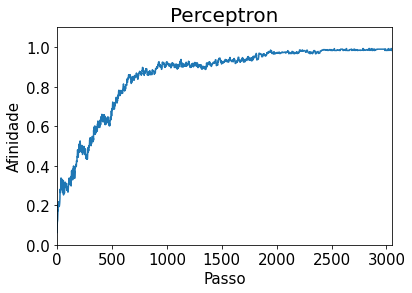
\includegraphics[width=0.5\textwidth]{img1.png}
            \centering
            \caption{Afinidade $\times$ nº de passos no simulador.}
            \label{img1}
 \end{figure}

Podemos perceber um comportamento que indica que o perceptron consegue aprender, sendo que o aprendizado ocorre mais rápido nos passos iniciais e se estabiliza em média muito próximo de $1$ por volta dos 2000 passos. Isso sugere que uma tendência de que o neurônio aprenda desde que permita que a rede seja executada uma quantidade suficiente de passos. É interessante notar que devido aos valores binários dos vetores, os valores que a afinidade pode assumir para uma única execução é discretizado, e a proximidade com o valor ideal para uma grande quantidade de passos indica que em uma parcela significativa das execuções o perceptron atingiu o peso objetivo.

Considerando que o sigmoide é um modelo de neurônio naturalmente mais sensível, e com o objetivo de testar a viabilidade deste modelo em computadores quânticos a longo prazo, para simular o sigmoide foi optado então em utilizar o simulador disponibilizado pelo Qiskit chamado `\textit{statevector\_simulator}'. Este simulador, diferente do anterior, não inclui ruídos, ele é um simulador de um circuito quântico ideal.

Observando a função de ativação podemos observar que as entradas (e pesos) aparecem sempre aos pares como argumentos de funções trigonométricas, dessa forma temos na realidade  $m-1$ parâmetros livres para $N$ qubits e $m=2^N$ estados. O que torna possível representar o mesmo resultado com apenas $m-1$ entradas (e pesos).  A partir destas considerações então foi simulado um neurônio com 3 entradas (2+1 qubits).

Seguindo um procedimento análogo ao perceptron, primeiro foi gerado um vetor peso objetivo ideal de 3 componentes definidas aleatoriamente, onde as componentes variam enter $0$ e $2\pi$. Estes valores posteriormente são então codificados como as fases dos coeficientes de amplitude do vetor de estado do sistema.

A partir disto é gerado então um conjunto de treinamento com 200 vetores de entrada definidos aleatoriamente e um  peso objetivo também aleatório. A saída ideal é então calculada e, após esta etapa, repetindo o processo adotado para o perceptron, o vetor peso objetivo é `esquecido' e é então gerado um novo vetor peso inicial de maneira aleatória.

Para o treinamento do sigmoide foi adotado um taxa de aprendizagem de $\nu=0.1$ e foram definidas duas condições de paradas: O treinamento deveria se encerrar ou se a função custo fosse reduzida para menos que $10^{-3}$ ou se ela começasse a aumentar. Após aproximadamente 4.000 passos, a função custo reduziu de um valor inicial de aproximadamente $5,75\times10^{-2}$ para aproximadamente $1.74\%$ do seu valor inicial, isto é $1,00\times10^{-3}$. Comportamento este que pode ser conferido na Figura \ref{img2}.

\begin{figure}[ht]
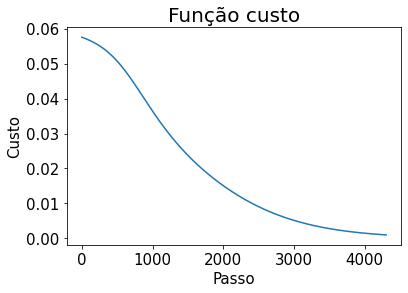
\includegraphics[width=0.5\textwidth]{custo.png}
\centering
\caption{Comportamento da função custo para o sigmoide no simulador. }
\label{img2}
\end{figure}

Como podemos perceber, a função custo sofre um decréscimo conforme era esperado, o que implica que o neurônio sigmoide está aprendendo a partir do conjunto de treinamento. Podemos observar também que com o conjunto de parâmetros que rodamos a rede neural, a função custo aparenta se estabilizar em $1,00\times10^{-3}$, não decrescendo para valores menores que este. Isto está de acordo com o fato de que o encerramento foi feito quando a função custo sofreu um acréscimo. Uma hipótese é que começaria a oscilar em torno deste valor. Caso desejar diminuir ainda mais a função custo, podemos pensar que poderíamos alterar  a taxa de aprendizagem, alterar o conjunto de dados de treinamento ou até mesmo utilizar um algoritmo de aprendizado diferente.

Por fim, temos o método kernel. Da mesma forma com o que fizemos no modelo sigmoide, utilizamos o `\textit{statevector\_simulator}'. Para satisfazer as condições discutidas anteriormente, o quadrado centralizado na origem possui um lado de $1.08$, isto é, os pontos podem ser gerados aleatoriamente nas coordenadas $\left(x,y\right)$ sendo $x,y\in\left[-0,54,0.54\right]$. Para o conjunto de treinamento foi gerado uma grade de pontos com espaçamento de $\Delta x=\Delta y=0.04$ entre si e o raio do círculo utilizado para calcular as saídas ideais foi de $0.42$, onde os pontos que estão fora do círculo foram considerados compondo a classe positiva ($+1$) e os pontos no interior compõem a classe negativa ($-1$), novamente, após esta etapa `esquecemos' o raio.

Utilizando estes critérios, então foi calculado um deslocamento $b\approx 0.15$. E a partir deste valor de deslocamento, geramos $100$ novos pontos aleatórios no interior do quadrado, destes pontos $99\%$ dos pontos foram classificados corretamente, mais especificamente, $100\%$ dos pontos no interior e $98\%$ dos pontos no exterior foram classificados corretamente. Isso sugere que o círculo que o método kernel aprendeu provavelmente possui um raio ligeiramente maior do que o círculo que utilizamos para gerar nosso conjunto de dados de treinamento. Algumas hipóteses que surgem que poderiam melhorar o resultado é encontrar uma razão entre o lado do quadrado e o raio do círculo com que o método funcione melhor, uma vez que durante este treinamento o raio foi escolhido empiricamente. Ou até mesmo trabalhar com outra superfície ao invés do cone, por exemplo um hiperboloide de uma ou duas folhas.
 
\subsection{Implementações dos modelos}

Uma vez que o modelo de aprendizado de máquina já tenha sido implementado no simulador utilizando o Qiskit, de maneira geral só precisamos realizar pequenas modificações no código original para executá-lo então em um dispositivo quântico real. Ao invés de enviar o circuito quântico para ser executado em um simulador local disponibilizado pela biblioteca Qiskit, o  submetemos para os dispositivos quânticos da IBM via nuvem através da mesma biblioteca, e em sequência obtemos o resultado. Sendo assim, os ajustes não são o maior desafio nesta etapa, porém os dispositivos reais disponíveis para acesso público gratuitamente ainda apresentam muitos desafios. Dentre eles podemos destacar uma quantidade significativa de ruídos,  limitações como a quantidade de qubits disponíveis, o tempo extra para submetermos o circuito e recebermos o resultado, e ainda frequentemente nos deparamos com filas de até centenas de códigos esperando para serem executados no mesmo dispositivo, tendo a vista a pouca oferta de opções, aumentando assim significativamente o tempo necessário para executar os treinamentos. 

O perceptron é o modelo que mais necessitou adaptações para ser implementado em um dispositivo real. Isto decorre do fato de que para implementarmos o modelo com 16 entradas como feito no simulador, além dos 4 qubits necessários para codificar a entrada e o qubit auxiliar (o que justificava a definição de 4+1 qubit utilizada anteriormente) foi necessário utilizar qubits adicionais para a aplicação do NOT multicontrolado. Porém a IBM Quantum Experience nos fornecesse acesso principalmente a dispositivos com apenas 5 qubits (ou menos), desta forma foi necessário reduzir o número de entradas do peceptron para 4 entradas e implementar um modelo de 2+1 qubit.

A metodologia adotada foi a mesma do simulador, porém com as diferenças de que agora temos 4 entradas, e o conjunto de treinamento é composto por 55 vetores, sendo que 5 resultam em uma saída positiva e 50 uma saída negativa. Além disso reduzimos o limite de passos a cada treinamento para 50 passos e foi executado no dispositivo `\textit{ibmq\_vigo}', que apresentou os melhores resultados dentre os dispositivos quânticos testados anteriormente. O resultado pode ser conferido na Figura \ref{pq}.

\begin{figure}[ht]
            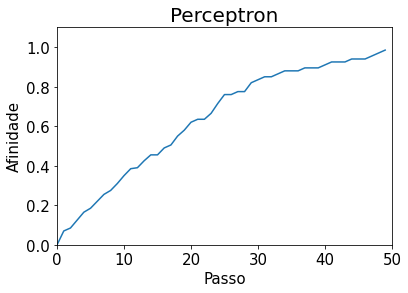
\includegraphics[width=0.5\textwidth]{pq.png}
            \centering
            \caption{Afinidade $\times$ nº de passos no dispositivo quântico.}
            \label{pq}
 \end{figure}

Podemos perceber um comportamento similar ao observado no simulador no sentido de que sugere uma tendência de que o perceptron aprenda uma vez que permitimos que ele seja executado por uma quantidade suficiente de passos. Também pode-se notar que ao diminuir pela metade a quantidade de entradas, foi necessário significativamente menos passos para obtermos uma média da afinidade próxima de 1.

Quanto ao sigmoide, considerando que é naturalmente um modelo mais sensível aos ruídos, pensou-se em utilizar um dispositivo quântico que apresentasse um desempenho melhor que os vistos até então, apesar das filas maiores de espera. Para compensar então foi reduzido o conjunto de treinamentos para 50 entradas e foi utilizado o dispositivo `\textit{ibmq\_santiago}'. O volume quântico, abreviado para QV do inglês (\textit{quantum volume}), é uma métrica que a IBM definiu para medir a performance dos seus computadores quânticos reais. Sendo assim, podemos encarar como uma quantificação desta performance, sendo que quanto maior o QV, melhor a performance do dispositvo. Dois dos três dispositivos utilizados até aqui (`\textit{ibmq\_valencia }' e `\textit{ibmq\_vigo }') possuem $QV=16$, enquanto o `\textit{ibmq\_5\_yorktown}' apresenta $QV=8$. A escolha do `\textit{ibmq\_santiago}' se deu por possuir $QV=32$.

Dito isso, foi necessário remover a condição de parada para o treinamento baseado simplesmente no aumento da função custo, uma vez que ela apresentou uma oscilação desde o começo. O resultado pode ser visualizado na Figura \ref{sq}. Paralelamente ao código executado `\textit{ibmq\_santiago}', também foi executado outro idêntico no dispositivo `\textit{ibmq\_5\_yorktown}' ($QV=8$), devido à filas menores, o resultado pode ser conferido na figura \ref{sq2}.

\begin{figure}[ht]
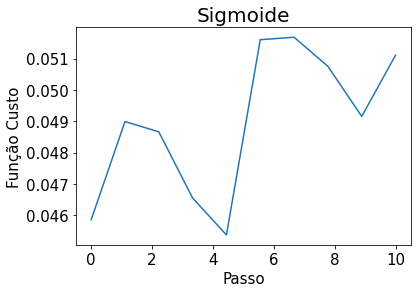
\includegraphics[width=0.5\textwidth]{sq1.png}
\centering
\caption{Comportamento da função custo para o sigmoide no dispositivo  `\textit{ibmq\_santiago}'. }
\label{sq}
\end{figure}
\begin{figure}[ht]
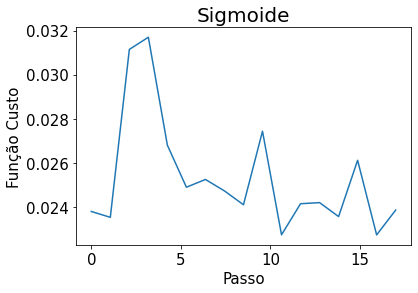
\includegraphics[width=0.5\textwidth]{sq2.png}
\centering
\caption{Comportamento da função custo para o sigmoide no dispositivo  `\textit{ibmq\_5\_yorktown}'. }
\label{sq2}
\end{figure}

Graficamente, podemos perceber que há um comportamento oscilatório. E calculando a média dos passos que foram possíveis de serem executados nos dispositivos quânticos reais,  10 no `\textit{ibmq\_santiago}' e 17 no `\textit{ibmq\_5\_yorktown}', temos que o valor custo foram em média $\left(4,90\pm0,23\right)\times10^{-2}$ e $\left(2,54\pm0,25\right)\times10^{-2}$, aproximadamente os mesmos valores iniciais ($4,59\times10^{-2}$ e $2,38\times10^{-2}$). Ou seja, apesar de mostrarmos que o modelo funciona em um dispositivo quântico ideal, ele não aparentou ter capacidade de aprendizagem em um dispositivo quântico real. A hipótese mais provável é que seja devido ao ruído. Para tentarmos melhorar este modelo visando dispositivos atuais ou de curto prazo, poderíamos levantar algumas hipóteses análogas ao discutido sobre como melhorar o modelo implementado no simulador, isto é, alterar a taxa de aprendizagem, o conjunto de dados de treinamento ou até o algoritmo de aprendizado implementado. 

Outro ponto é que enquanto o modelo no simulador teve aproximadamente 4.000 passos, no dispositivo quântico tivemos tempo de executar apenas  $1$2 devido ao elevado número de cálculos que é necessário serem executados em um dispositivo quântico e as políticas de acesso da IBM aos seus dispositivos públicos. Porém, vale lembrar que em nenhum momento a função custo no simulador aumentou nestes 4.000 passos, enquanto no dispositivo quântico real parece estar flutuando em torno do valor inicial desde o começo, o que é uma característica esperada tendo em vista os problemas de ruídos que os dispositivos atuais ainda enfrentam, uma vez que o modelo sigmoide foi construído para ser sensível a pequenas mudanças. Porém fica em aberto a possibilidade de permitir que o sigmoide rode mais tempo para verificar se em algum momento há alguma tendência de que o neurônio esteja aprendendo, mesmo com os ruídos presentes nos dispositivos atuais.

E por fim temos o método kernel, que diferente dos modelos anteriores não apresenta um processo de aprendizagem gradual que nos permita interromper no meio do processo e obter um resultado parcial para investigarmos alguma tendência de comportamento como fizemos com o sigmoide. Se executado o algoritmo sob as mesmas condições das quais implementamos no simulador, necessitaríamos semanas ou mesmo meses, dependendo das condições, para conseguirmos calcular apenas o deslocamento. Desta forma forma optou-se por diminuir o conjunto de dados de treinamento.

Com esta ideia, foi gerado então uma grade de pontos espaçado $\Delta x= \Delta y = 0.08$ entre si dentro do domínio $x,y\in\left[-0,52,0.52\right]$, dessa forma reduziu-se significativamente a quantidade de cálculos necessários. Porém isto aconteceu em troca de precisão, agora utilizando o dispositivo quântico `\textit{ibmq\_vigo }' nosso deslocamento foi de aproximadamente $7,87\times10^{-2}$, aproximadamente $1/2$ do valor obtido no simulador. Além dos desafios habituais de utilizar os dispositivos quânticos reais da IBM, durante o período reservado para a implementação do método kernel, a IBM emitiu um alerta de manutenção, no qual comunicou a aposentadoria de alguns dispositivos quânticos nos próximos dias (incluindo o `\textit{ibmq\_vigo}')  e o desligamento temporário de outros, comunicando que isto resultaria em filas de espera ainda maiores para  a utilização dos dispositivos durante o período atual.

Então, tendo em vista em vista a limitação de tempo no desenvolvimento do TCC, e a situação que se apresentou, optou-se por executar apenas o treinamento (ou seja, o cálculo do deslocamento) no dispositivo quântico. Esta escolha decorre do fato que uma vez que temos $p$ vetores da classe positiva e $n$ vetores da classe negativa no nosso conjunto do treinamento, o cálculo do deslocamento vai exigir que sejam computados $n^2+p^2$ produtos internos, enquanto a classificação de um novo ponto necessita da computação de apenas $n+p$ produtos internos. Desta forma, optou-se que o cálculo mais pesado fosse executado no computador quântico. 

Utilizando então o circuito implementado no simulador com o peso obtido no dispositivo quântico, classificamos $100$ novos pontos. Destes $54\%$ foram classificados corretamente, porém $100\%$ dos pontos gerados no interior do círculo e aproximadamente $20\%$ dos pontos no exterior. Logo, o raio estimado pelo método consideravelmente maior que o utilizado na fase de geração dos dados de treinamento.

Além da mesma discussão realizada no simulador (como a razão entre os lados do quadrado e o raio do círculo, e a própria superfície em 3 dimensões) este modelo não  dá muitas alternativas para melhorar a precisão além de aumentar o conjunto de dados treinamentos ou utilizar um dispositivo com maior precisão. Porém os dispositivos que podem ser utilizados a curto prazo como os dispositivos da IBM apresentam tanto uma quantidade considerável de ruído como filas relativamente longas, exigindo uma grande quantidade de tempo. Fica em aberto a possibilidade de que valia mais apena esperar que um incremento na qualidade dos dispositivo quânticos reais de acesso público, uma vez que já podemos verificar que é um modelo que funciona em um dispositivo ideal.



\chapter{Conclusão}

Sintetizando então os resultados obtidos durante este trabalho, baseado em um artigo de 2019 \cite{Italiano} foram implementados dois algoritmos para cálculo do produto interno entre vetores binários em um computador quântico. Porém, diferindo dos resultados obtidos na literatura, não foi possível verificar diferença significativa entre os resultados obtidos por cada algoritmo, isto é, as discrepâncias obtida ao calcular o mesmo produto interno  no mesmo dispositivo, porém utilizando os dois algoritmos diferentes, não apresentaram diferença significativa entre si. O mesmo pode-se dizer da adaptação que foi proposta e implementada para vetores de valores contínuos. Dentre as hipóteses levantadas para explicar essa discrepância, a principal é a arquitetura dos processadores quânticos.

Quanto aos modelos híbridos de aprendizado de máquina, os três modos foram implementados em simuladores disponibilizados pelo Qiskit, e apresentaram resultados satisfatórios que demonstram um bom potencial quanto à capacidade de aprendizagem de cada modelo. Já sobre a implementação em dispositivos reais, de maneira geral se destaca o problema quanto à demora no processo de submissão do circuito e obtenção de seu resultado, sendo que este problema se sobressaiu quando foi implementado o método kernel, que ainda sofreu o agravante de uma manutenção nos servidores da IBM. Outra dificuldade bastante notável na implementação dos modelos em dispositivos reais são os ruídos, sendo que este problema é notado principalmente durante a implementação do modelo sigmoide, uma vez que foi construído para ser sensível a pequenas variações. Já o perceptron simulado se destaca por ter se mostrado um modelo relativamente robusto quanto aos ruídos e tendo sido capaz de aprender a partir do conjunto de treinamento tanto no simulador quanto no dispositivo real.

Porém vale a pena lembrar que tanto a qualidade do acesso a dispositivos quânticos reais, quanto o problema do ruído nestes dispositivos, são problemas que acredita-se que devem ser mitigados com um maior desenvolvimento tecnológico. Então, uma vez que os modelos se mostram eficientes em um computador idealizado, é coerente supor que venham a ser eficientes em dispositivos reais no futuro. Além disso, outros possíveis caminho para o desenvolvimento futuro deste trabalho é tanto desenvolver os modelos sigmoide e kernel para serem mais tolerantes aos ruídos, quanto desenvolver os modelos para serem mais complexos e/ou eficientes mesmo que ainda em modelos idealizados. Um exemplo que pode-se citar é a implementação de múltiplos qubits em um único computador quântico ou também implementar a etapa de treinamento dos modelos de redes neurais nos computadores quânticos.

Por fim, pode-se destacar que a parte mais desafiadora do trabalho consistiu no estudo e compreensão da modelagem do circuito quântico. Compreender a teoria geral no qual o cálculo dos produtos internos foi construído exigiu conhecimentos de mecânica quântica e computação quântica. Porém uma vez compreendido, permitiu não só implementar o produto interno entre valores binários para o perceptron, como consta na literatura, mas também adaptar para os valores contínuos para os sigmoide e ainda fazer uma adaptação mais extrema para o método kernel. Desta forma, foi demonstrada a viabilidade de uma generalização do perceptron para um modelo de valores contínuos e foi construído um modelo baseado no método kernel que além de ser capaz de efetivamente aprender em dispositivos ideais, serve como uma introdução interessante à área.

Concluindo então, dessa forma acreditamos que o trabalho representa mais um passo no caminho certo do desenvolvimento da inteligência artificial quântica.

\bibliografia{referencias}  

\apendice 

\chapter{Códigos}

Abaixo, segue o código desenvolvido durante este projeto. Algumas observações são necessárias. Primeiramente, todo ele foi desenvolvido no Google Colab. Portanto, este código em Python é uma conversão do documento original que possui o formato .ipynb. Esta extensão, diferente de um script tradicional de Python, oferece a possibilidade de executar somente trechos do código (chamado de células) na ordem de nosso interesse. Sendo assim, o código abaixo contém múltiplos trechos de códigos que são executados não necessariamente em ordem linear. Para facilitar o início de cada nova célula será informada através de um comentário.

Além disso, vale lembrar que apesar do código das implementações nos dispositivos quânticos do sigmoide e kernel estarem também no Google Colab, à fins de organização, eles foram implementados separadamente em um computador pessoal, conforme mencionado no texto. E por fim, apesar de todo o código estar reunido em um único documento, há na realidade 14 códigos principais que poderiam compor arquivos distintos: As implementações dos  2 algoritmos de produto interno (binário e contínuo, em um dispositivo quântico real e no simulador)  e a implementação dos 3 modelos (no simulador e dispositivo quântico), além de funções auxiliares que ajudaram a verificar a consistência dos códigos. Isto explica porque alguns trechos de código aparecem repetidos em mais de um trecho no decorrer do arquivo, assim como a extensão do mesmo.

\begin{verbatim}
# -*- coding: utf-8 -*-
"""TCC.ipynb
Automatically generated by Colaboratory."""
\end{verbatim}

\section{Bibliotecas necessárias}

\begin{verbatim}
# Célula 1
!pip install qiskit #Instala o Qiskit
from google.colab import drive
\end{verbatim}

\section{Especificações técnicas}

\begin{verbatim}
# Célula 2
import qiskit

# Célula 3
qiskit.__version__

# Célula 4
qiskit.__qiskit_version__

# Célula 5
!cat /proc/cpuinfo

# Célula 6
!cat /proc/meminfo
\end{verbatim}

\section{Discrepância}
\subsection{Preparação}

\begin{verbatim}
# Célula 7
from qiskit import IBMQ                       # Biblioteca para login no IBMQ
IBMQ.save_account('')
IBMQ.load_account()                           # Carregamos a conta
# Carregamos biblioteca científica numpy
import numpy as np                       
# Importamos tudo as funções principais
from qiskit import *                          
# Função pra monitorar nosso trabalho no servidor
from qiskit.tools.monitor import job_monitor  
import random

# Célula 8
# Funções
# Bloco de mudança de sinal
def flip(b,l):
    # b - Bit que queremos mudar o sinal
    # l - Ângulo que deve rotacionar
    cq = QuantumCircuit(3,1)    # Criamos nosso circuito 
    # Primeiro vamos converter nosso número para binário
    binario=bin(b).replace('0b','')
    while((len(binario)<2)):
        binario='0'+binario
    #Se é 0,  aplicamos:
    if (0==int(binario[0])):
        cq.x(0)
    if (0==int(binario[1])):
        cq.x(1)
    # PARTE 2: Aplicamos o Z multicontrolado:
    if (abs(l)==np.pi):
      cq.cz(0,1)
    else:
      cq.cu1(l,0,1)
    #Se é 0,  aplicamos:
    if (0==int(binario[1])):
        cq.x(1)
    if (0==int(binario[0])):
        cq.x(0)
    return(cq)
\end{verbatim}
\subsection{Binário}
\subsubsection{Vetores e Funções}

\begin{verbatim}
# Célula 9
# Lista de vetores
vet = {
    "0":  np.array([[-1],[-1],[-1],[-1]])/2,
    "1":  np.array([[-1],[-1],[-1],[ 1]])/2,
    "2":  np.array([[-1],[-1],[ 1],[-1]])/2,
    "3":  np.array([[-1],[-1],[ 1],[ 1]])/2,
    "4":  np.array([[-1],[ 1],[-1],[-1]])/2,
    "5":  np.array([[-1],[ 1],[-1],[ 1]])/2,
    "6":  np.array([[-1],[ 1],[ 1],[-1]])/2,
    "7":  np.array([[-1],[ 1],[ 1],[ 1]])/2,
    "8":  np.array([[ 1],[-1],[-1],[-1]])/2,
    "9":  np.array([[ 1],[-1],[-1],[ 1]])/2,
    "10":  np.array([[ 1],[-1],[ 1],[-1]])/2,
    "11":  np.array([[ 1],[-1],[ 1],[ 1]])/2,
    "12":  np.array([[ 1],[ 1],[-1],[-1]])/2,
    "13":  np.array([[ 1],[ 1],[-1],[ 1]])/2,
    "14":  np.array([[ 1],[ 1],[ 1],[-1]])/2,
    "15":  np.array([[ 1],[ 1],[ 1],[ 1]])/2
}
\end{verbatim}

\subsubsection{Simulações}

\begin{verbatim}
# Célula 10
#RESULTADO TEÓRICO
O=np.zeros((16, 16))
for l in (range(16)):
    for c in (range(16)):
        res=vet[str(l)].transpose().dot(vet[str(c)])[0][0]
        res=np.power(res,2)
        O[l][c]=res

# Célula 11
# Bloco de rotação
R_sim=np.zeros((16, 16))
for l in (range(16)):
    for c in (range(16)):
        i=vet[str(l)]
        w=vet[str(c)]
        cq = QuantumCircuit(3,1)    # Criamos nosso circuito        
        # OPERADOR DE ENTRADA
        ## Aplicamos a porta de Hadamard
        cq.h(0)                     # Aplicamos hadamard no qubit 0
        cq.h(1)                     # Aplicamos hadamard no qubit 1        
        ## Mudança de sinal
        for k in (range(4)):
            if (i[k][0]<0):
                cq=cq+flip(k,np.pi)
        #OPERADOR PESO
        ## Mudança de sinal
        for k in (range(4)):
            if (w[k][0]<0):
                cq=cq+flip(k,-np.pi)
        ## Porta de Hadamard
        cq.h(0)                     # Aplicamos hadamard no qubit 0
        cq.h(1)                     # Aplicamos hadamard no qubit 1
        ## Porta X
        cq.x(0)                     # Aplicamos X no qubit 0
        cq.x(1)                     # Aplicamos X no qubit 1
        #MEDIÇÃO
        cq.ccx(0,1,2)    # Aplicamos a porta de Toffoli
        # Escolhemos nosso backend
        backend = BasicAer.get_backend('statevector_simulator')  
        # Executamos e pegamos o resultado
        result = execute(cq, backend).result()           
        # Pegamos o vetor de estados
        psi  = result.get_statevector(cq)                        
        res=(psi[len(psi)-1].conjugate()*psi[len(psi)-1])
        print(res)
        R_sim[l][c]=res.real

# Célula 12
# HSGS
R_sim2=np.zeros((16, 16))
for l in (range(16)):
    for c in (range(16)):
        i=vet[str(l)]
        w=vet[str(c)]
        cq = QuantumCircuit(3,1)    # Criamos nosso circuito        
        # OPERADOR DE ENTRADA
        ## Aplicamos a porta de Hadamard
        if (i[0]>0):        
            cq.h(0)                     # Aplicamos hadamard no qubit 0
            cq.h(1)                     # Aplicamos hadamard no qubit 1        
            if (i[2]<0): cq.z(0)
            if (i[1]<0): cq.z(1)
            if (i[2]*i[1]!=i[3]*0.5): cq.cz(0,1) 
        elif(i[0]<0):
            cq.u3(-3*np.pi/2,0,np.pi,0)
            cq.h(1)            
            if (i[2]>0): cq.z(0)
            if (i[1]>0): cq.z(1)
            if (i[2]*i[1]==i[3]*0.5): cq.cz(0,1) 
        #OPERADOR PESO
        if(w[0]>0):
            if (w[2]*w[1]!=w[3]*0.5): cq.cz(0,1) 
            if (w[1]<0): cq.z(1)
            if (w[2]<0): cq.z(0)
            cq.h(0)                     # Aplicamos hadamard no qubit 0
            cq.h(1)                     # Aplicamos hadamard no qubit 1
        elif(w[0]<0):
            if (w[2]*w[1]==w[3]*0.5): cq.cz(0,1) 
            if (w[1]>0): cq.z(1)
            if (w[2]>0): cq.z(0)
            cq.u3(-3*np.pi/2,0,np.pi,0)
            cq.h(1)
        ## Porta X
        cq.x(0)                     # Aplicamos X no qubit 0
        cq.x(1)                     # Aplicamos X no qubit 1
        #MEDIÇÃO
        cq.ccx(0,1,2)    # Aplicamos a porta de Toffoli
        backend = BasicAer.get_backend('statevector_simulator')    
        result = execute(cq, backend).result()                   
        psi  = result.get_statevector(cq)                        
        res=(psi[len(psi)-1].conjugate()*psi[len(psi)-1])
        R_sim2[l][c]=res.real

# Célula 13
#Discrepância Blocos
d=0
for x in range(16):
    for y in range(16):
        d=d+abs(O[x][y]-R_sim[x][y])
d=d/256
print(d)

# Célula 14
#Discrepância HSGS
d=0
for x in range(16):
    for y in range(16):
        d=d+abs(O[x][y]-R_sim2[x][y])
d=d/256
print(d)
\end{verbatim}
\subsubsection{Resultados}
\begin{verbatim}
# Célula 15
#RESULTADO TEÓRICO
O=np.zeros((16, 16))
for l in (range(16)):
    for c in (range(16)):
        res=vet[str(l)].transpose().dot(vet[str(c)])[0][0]
        res=np.power(res,2)
        O[l][c]=res

# Célula 16
# Bloco de mudança de sinal
R_IBM=np.zeros((16, 16))
# Selecionamos um provedor aberto
provedor = IBMQ.get_provider(hub='ibm-q', group='open', project='main')
backend = provedor.get_backend('ibmq_vigo')    # Selecionamos um backend
for l in (range(16)):
    for c in (range(16)):
        i=vet[str(l)]
        w=vet[str(c)]
        cq = QuantumCircuit(3,1)    # Criamos nosso circuito        
        # OPERADOR DE ENTRADA
        ## Aplicamos a porta de Hadamard
        cq.h(0)                     # Aplicamos hadamard no qubit 0
        cq.h(1)                     # Aplicamos hadamard no qubit 1        
        ## Mudança de sinal
        for k in (range(4)):
            if (i[k][0]<0):
                cq=cq+flip(k,np.pi)
        #OPERADOR PESO
        ## Mudança de sinal
        for k in (range(4)):
            if (w[k][0]<0):
                cq=cq+flip(k,-np.pi)
        ## Porta de Hadamard
        cq.h(0)                     # Aplicamos hadamard no qubit 0
        cq.h(1)                     # Aplicamos hadamard no qubit 1
        ## Porta X
        cq.x(0)                     # Aplicamos X no qubit 0
        cq.x(1)                     # Aplicamos X no qubit 1
        #MEDIÇÃO
        cq.ccx(0,1,2)    # Aplicamos a porta de Toffoli
        cq.measure(2,0)  # Medimos
        # Submetemos nosso trabalho ao servidor
        trabalho_ibm = execute(cq, backend=backend)     
        job_monitor(trabalho_ibm)
        resultado = trabalho_ibm.result()      # Obtemos o resultado
        contagem = resultado.get_counts(cq)    # Acessamos a contagem
        try:
            res= contagem['1']/1024
        except:
            res=0
        R_IBM[l][c]=res

# Célula 17
# HSGS 
R_IBM2=np.zeros((16, 16))
provedor = IBMQ.get_provider(hub='ibm-q', group='open', project='main')         
backend = provedor.get_backend('ibmq_vigo')    # Selecionamos um backend
for l in (range(16)):
    for c in (range(16)):
        i=vet[str(l)]
        w=vet[str(c)]
        cq = QuantumCircuit(3,1)    # Criamos nosso circuito        
        # OPERADOR DE ENTRADA
        ## Aplicamos a porta de Hadamard
        if (i[0]>0):        
            cq.h(0)                     # Aplicamos hadamard no qubit 0
            cq.h(1)                     # Aplicamos hadamard no qubit 1        
            if (i[2]<0): cq.z(0)
            if (i[1]<0): cq.z(1)
            if (i[2]*i[1]!=i[3]*0.5): cq.cz(0,1) 
        elif(i[0]<0):
            cq.u3(-3*np.pi/2,0,np.pi,0)
            cq.h(1)            
            if (i[2]>0): cq.z(0)
            if (i[1]>0): cq.z(1)
            if (i[2]*i[1]==i[3]*0.5): cq.cz(0,1) 
        #OPERADOR PESO
        if(w[0]>0):
            if (w[2]*w[1]!=w[3]*0.5): cq.cz(0,1) 
            if (w[1]<0): cq.z(1)
            if (w[2]<0): cq.z(0)
            cq.h(0)                     # Aplicamos hadamard no qubit 0
            cq.h(1)                     # Aplicamos hadamard no qubit 1
        elif(w[0]<0):
            if (w[2]*w[1]==w[3]*0.5): cq.cz(0,1) 
            if (w[1]>0): cq.z(1)
            if (w[2]>0): cq.z(0)
            cq.u3(-3*np.pi/2,0,np.pi,0)
            cq.h(1)
        ## Porta X
        cq.x(0)                     # Aplicamos X no qubit 0
        cq.x(1)                     # Aplicamos X no qubit 1
        #MEDIÇÃO
        cq.ccx(0,1,2)    # Aplicamos a porta de Toffoli
        cq.measure(2,0)  # Medimos
        trabalho_ibm = execute(cq, backend=backend)     
        job_monitor(trabalho_ibm)
        resultado = trabalho_ibm.result()      # Obtemos o resultado
        contagem = resultado.get_counts(cq)    # Acessamos a contagem
        try:
            res= contagem['1']/1024
        except:
            res=0
            
        R_IBM2[l][c]=res

# Célula 18
#Discrepância Blocos
d=0
for x in range(16):
    for y in range(16):
        d=d+abs(O[x][y]-R_IBM[x][y])
d=d/256
print(d)

# Célula 19
#Discrepância HSGS
d=0
for x in range(16):
    for y in range(16):
        d=d+abs(O[x][y]-R_IBM2[x][y])
d=d/256
print(d)
\end{verbatim}
\subsection{Não-binário}
\subsubsection{Vetores e Funções}
\begin{verbatim}
# Célula 20
# Vetores aleatórios
e=[]
for x in range(8):
    e.append([random.randint(0,341)/100,
              random.randint(0,341)/100,
              random.randint(0,341)/100,
              random.randint(0,341)/100])
tam=len(e)
\end{verbatim}
\subsubsection{Simulações}
\begin{verbatim}
# Célula 21
O=np.zeros((tam, tam))
#RESULTADO TEÓRICO
for l in (range(len(e))):
    for c in (range(len(e))):
        v1=np.array([[np.cos(e[l][0])+np.sin(e[l][0])*1j],
                     [np.cos(e[l][1])+np.sin(e[l][1])*1j],
                     [np.cos(e[l][2])+np.sin(e[l][2])*1j],
                     [np.cos(e[l][3])+np.sin(e[l][3])*1j]])/2
        v2=np.array([[np.cos(e[c][0])+np.sin(e[c][0])*1j],
                     [np.cos(e[c][1])+np.sin(e[c][1])*1j],
                     [np.cos(e[c][2])+np.sin(e[c][2])*1j],
                     [np.cos(e[c][3])+np.sin(e[c][3])*1j]])/2
        res=v1.conjugate().transpose().dot(v2)[0][0]
        res=res.conjugate()*res
        O[l][c]=res.real

# Célula 22
# Bloco de rotação de fase
R_sim=np.zeros((tam, tam))
for l in (range(len(e))):
    for c in (range(len(e))):
        i=e[l]
        w=e[c]
        cq = QuantumCircuit(3,1)    # Criamos nosso circuito        
        # OPERADOR DE ENTRADA
        ## Aplicamos a porta de Hadamard
        cq.h(0)                     # Aplicamos hadamard no qubit 0
        cq.h(1)                     # Aplicamos hadamard no qubit 1        
        ## Mudança de sinal
        for k in (range(4)):
            if (i[k]!=0):               
                cq=cq+flip(k,i[k])
        #OPERADOR PESO
        ## Mudança de sinal
        for k in (range(4)):
            if (w[k]!=0):
                cq=cq+flip(k,-w[k])
        ## Porta de Hadamard
        cq.h(0)                     # Aplicamos hadamard no qubit 0
        cq.h(1)                     # Aplicamos hadamard no qubit 1
        ## Porta X
        cq.x(0)                     # Aplicamos X no qubit 0
        cq.x(1)                     # Aplicamos X no qubit 1
        #MEDIÇÃO
        cq.ccx(0,1,2)    # Aplicamos a porta de Toffoli
        backend = BasicAer.get_backend('statevector_simulator')
        result = execute(cq, backend).result()                   
        psi  = result.get_statevector(cq)                        
        res=(psi[len(psi)-1].conjugate()*psi[len(psi)-1])
        R_sim[l][c]=res.real

# Célula 23
#HSGS
R_sim2=np.zeros((tam, tam))
for l in (range(len(e))):
    for c in (range(len(e))):
        i=e[l]
        w=e[c]
        cq = QuantumCircuit(3,1)    # Criamos nosso circuito        
        # OPERADOR DE ENTRADA
        ## Aplicamos a porta de Hadamard
        i=e[l]
        w=e[c]
        cq = QuantumCircuit(3,1)    # Criamos nosso circuito        
        # OPERADOR DE ENTRADA
        ## Aplicamos a porta de Hadamard
        cq.h(0)                     # Aplicamos hadamard no qubit 0
        cq.h(1)                     # Aplicamos hadamard no qubit 1     
        cq.u1(i[1],0)
        cq.u1(i[2],1)
        cq.cu1(i[0]-(i[1]+i[2]),0,1)
        cq.x(0)
        cq.x(1)
        cq.cu1(i[3],0,1)
        #OPERADOR PESO
        cq.cu1(-w[3],0,1)
        cq.x(0)
        cq.x(1)
        cq.cu1(-w[0]+(w[1]+w[2]),0,1)
        cq.u1(-w[1],0)
        cq.u1(-w[2],1)
        ## Porta de Hadamard
        cq.h(0)                     # Aplicamos hadamard no qubit 0
        cq.h(1)                     # Aplicamos hadamard no qubit 1
        ## Porta X
        cq.x(0)                     # Aplicamos X no qubit 0
        cq.x(1)                     # Aplicamos X no qubit 1
        #MEDIÇÃO
        cq.ccx(0,1,2)    # Aplicamos a porta de Toffoli
        backend = BasicAer.get_backend('statevector_simulator')    
        result = execute(cq, backend).result()                  
        psi  = result.get_statevector(cq)                        
        res=(psi[len(psi)-1].conjugate()*psi[len(psi)-1])
        R_sim2[l][c]=res.real

# Célula 24
#Discrepância Blocos
d=0
for x in range(tam):
    for y in range(tam):
        d=d+abs(O[x][y]-R_sim[x][y])
d=d/(tam*tam)
print(d)

# Célula 25
#Discrepância HSGS
d=0
for x in range(tam):
    for y in range(tam):
        d=d+abs(O[x][y]-R_sim2[x][y])
d=d/(tam*tam)
print(d)
\end{verbatim}

\subsubsection{Resultados}

\begin{verbatim}
# Célula 26
O=np.zeros((tam, tam))
#RESULTADO TEÓRICO
for l in (range(len(e))):
    for c in (range(len(e))):
        v1=np.array([[np.cos(e[l][0])+np.sin(e[l][0])*1j],
                     [np.cos(e[l][1])+np.sin(e[l][1])*1j],
                     [np.cos(e[l][2])+np.sin(e[l][2])*1j],
                     [np.cos(e[l][3])+np.sin(e[l][3])*1j]])/2
        v2=np.array([[np.cos(e[c][0])+np.sin(e[c][0])*1j],
                     [np.cos(e[c][1])+np.sin(e[c][1])*1j],
                     [np.cos(e[c][2])+np.sin(e[c][2])*1j],
                     [np.cos(e[c][3])+np.sin(e[c][3])*1j]])/2
        res=v1.conjugate().transpose().dot(v2)[0][0]
        res=res.conjugate()*res
        O[l][c]=res.rea8

# Célula 27
#Bloco de rotação de sinal
R_IBM=np.zeros((tam, tam))
provedor = IBMQ.get_provider(group='open')           
backend = provedor.get_backend('ibmq_vigo')    # Selecionamos um backend
for l in (range(len(e))):
    for c in (range(len(e))):
        i=e[l]
        w=e[c]
        cq = QuantumCircuit(3,1)    # Criamos nosso circuito        
        # OPERADOR DE ENTRADA
        ## Aplicamos a porta de Hadamard
        cq.h(0)                     # Aplicamos hadamard no qubit 0
        cq.h(1)                     # Aplicamos hadamard no qubit 1        
        ## Mudança de sinal
        for k in (range(4)):
            if (i[k]!=0):
                cq=cq+flip(k,i[k])
        #OPERADOR PESO
        ## Mudança de sinal
        for k in (range(4)):
            if (w[k]!=0):
                cq=cq+flip(k,-w[k])
        ## Porta de Hadamard
        cq.h(0)                     # Aplicamos hadamard no qubit 0
        cq.h(1)                     # Aplicamos hadamard no qubit 1
        ## Porta X
        cq.x(0)                     # Aplicamos X no qubit 0
        cq.x(1)                     # Aplicamos X no qubit 1
        #MEDIÇÃO
        cq.ccx(0,1,2)    # Aplicamos a porta de Toffoli
        cq.measure(2,0)  # Medimos
        trabalho_ibm = execute(cq, backend=backend)    
        job_monitor(trabalho_ibm)
        resultado = trabalho_ibm.result()       # Obtemos o resultado
        contagem = resultado.get_counts(cq)     # Acessamos a contagem
        try:
            res= contagem['1']/1024
        except:
            res=0
        R_IBM[l][c]=res

# Célula 28
#HSGS
R_IBM2=np.zeros((tam, tam))
provedor = IBMQ.get_provider(group='open')          
backend = provedor.get_backend('ibmq_vigo')    # Selecionamos um backend
for l in (range(len(e))):
    for c in (range(len(e))):
        i=e[l]
        w=e[c]
        cq = QuantumCircuit(3,1)    # Criamos nosso circuito        
        # OPERADOR DE ENTRADA
        ## Aplicamos a porta de Hadamard
        cq.h(0)                     # Aplicamos hadamard no qubit 0
        cq.h(1)                     # Aplicamos hadamard no qubit 1     
        cq.u1(i[1],0)
        cq.u1(i[2],1)
        cq.cu1(i[0]-(i[1]+i[2]),0,1)
        cq.x(0)
        cq.x(1)
        cq.cu1(i[3],0,1)
        #OPERADOR PESO
        cq.cu1(-w[3],0,1)
        cq.x(0)
        cq.x(1)
        cq.cu1(-w[0]+(w[1]+w[2]),0,1)
        cq.u1(-w[1],0)
        cq.u1(-w[2],1)
        ## Porta de Hadamard
        cq.h(0)                     # Aplicamos hadamard no qubit 0
        cq.h(1)                     # Aplicamos hadamard no qubit 1
        ## Porta X
        cq.x(0)                     # Aplicamos X no qubit 0
        cq.x(1)                     # Aplicamos X no qubit 1
        #MEDIÇÃO
        cq.ccx(0,1,2)    # Aplicamos a porta de Toffoli
        cq.measure(2,0)  # Medimos
        trabalho_ibm = execute(cq, backend=backend)    
        job_monitor(trabalho_ibm)
        resultado = trabalho_ibm.result()       # Obtemos o resultado
        contagem = resultado.get_counts(cq)     # Acessamos a contagem
        try:
            res= contagem['1']/1024
        except:
            res=0
        R_IBM2[l][c]=res

# Célula 29
d=0
for x in range(tam):
    for y in range(tam):
        d=d+abs(O[x][y]-R_IBM[x][y])
        
d=d/(len(e)*len(e))
print(d)

# Célula 30
d=0
for x in range(tam):
    for y in range(tam):
        d=d+abs(O[x][y]-R_IBM2[x][y])
d=d/(len(e)*len(e))
print(d)
\end{verbatim}
\section{Perceptron}
\subsubsection{Simulador}
\begin{verbatim}
# Célula 31
# Bibliotecas
from qiskit import QuantumCircuit,Aer,execute             
import numpy as np                        
import random
import copy
from google.colab import files

# Célula 32
# Funções para montagem do Circuito quântico
# Porta CCCz
def cccz():
   cq = QuantumCircuit(7,1)
   cq.cu1(np.pi/4,0,3)  
   cq.cx(0,1)  
   cq.cu1(-np.pi/4,1,3)  
   cq.cx(0,1) 
   cq.cu1(np.pi/4,1,3)  
   cq.cx(1,2) 
   cq.cu1(-np.pi/4,2,3) 
   cq.cx(0,2) 
   cq.cu1(np.pi/4,2,3)
   cq.cx(1,2) 
   cq.cu1(-np.pi/4,2,3)
   cq.cx(0,2) 
   cq.cu1(np.pi/4,2,3)
   return (cq)
# Porta CCCCx
def ccccx():
    cq = QuantumCircuit(7,1)
    cq.ccx(0,1,5)
    cq.ccx(2,3,6)
    cq.ccx(5,6,4)
    cq.ccx(2,3,6)
    cq.ccx(0,1,5)
    return (cq)
# Bloco de Mudança de sinal
def flip(b):
    #b - Bit identiicando o estado
    cq = QuantumCircuit(7,1)    # Criamos nosso circuito 
    binario=bin(b).replace('0b','')
    while((len(binario)<4)):
        binario='0'+binario
    if (0==int(binario[0])):
        cq.x(0)
    if (0==int(binario[1])):
        cq.x(1)
    if (0==int(binario[2])):
        cq.x(2)
    if (0==int(binario[3])):
        cq.x(3)
    cq=cq+cccz()
    if (0==int(binario[3])):
        cq.x(3)
    if (0==int(binario[2])):
        cq.x(2)
    if (0==int(binario[1])):
        cq.x(1)
    if (0==int(binario[0])):
        cq.x(0)
    return(cq)
# Montagem do circuito
def circuito(e,p):
    #e - Lista com os vetores de entrada
    #p - Lista com os vetores peso
    cq = QuantumCircuit(7,1)
    cq.h(0)
    cq.h(1)                     
    cq.h(2)                    
    cq.h(3)                     
    for k in (range(16)):
        if (e[k][0]<0):
            cq=cq+flip(k)
    for k in (range(16)):
        if (p[k][0]<0):
            cq=cq+flip(k)
    cq.h(0)                   
    cq.h(1)                 
    cq.h(2)                   
    cq.h(3)                     
    cq.x(0)                     
    cq.x(1)                    
    cq.x(2)                    
    cq.x(3)                    
    return(cq)
# Configuração da simulação
def simulacao(cq,m):
    #cq - Circuito quântico a ser simulado
    #m  - Quantidades de repetições do simulador
    backend = Aer.get_backend('qasm_simulator')   # Nosso backend
    cq=cq+ccccx()
    cq.measure(4,0)  
    trabalho = execute(cq, backend, shots=m) 
    resultado = trabalho.result()
    contagem = resultado.get_counts(cq)             
    try:
        # A quantidade de vezes que mediu 1 sobre a quantidade total
        res = contagem['1']/m                       
    except:
       res=0    
    return (res)

# Célula 33
# Funções para geração/manipulação dos dados de treinamento
# Peso objetivo
def po():
    return (np.array([[+1],[+1],[+1],[+1],
                      [+1],[+1],[-1],[+1],
                      [+1],[-1],[-1],[-1],
                      [+1],[+1],[-1],[+1]],dtype='float')/4)
# Peso inicial
def pi():
    return (np.array([[+1],[+1],[-1],[+1],
                      [-1],[-1],[+1],[+1],
                      [+1],[-1],[+1],[+1],
                      [+1],[+1],[-1],[+1]],dtype='float')/4)
# Geração de dados de treinamento
def gerar_dados():
    e=[] 
    s=[] 
    pos=0 
    neg=0  
    p=po()
    positivos=50
    negativos=300
    total=(positivos+negativos)
    while(len(e)<total):
        progresso=((len(e))/total)*100
        if(progresso%10==0 or progresso>95):
            print(progresso)
        i=np.array([[(random.randint(0, 1)*2-1)/4],
                [(random.randint(0, 1)*2-1)/4],
                [(random.randint(0, 1)*2-1)/4],
                [(random.randint(0, 1)*2-1)/4],
                [(random.randint(0, 1)*2-1)/4],
                [(random.randint(0, 1)*2-1)/4],                    
                [(random.randint(0, 1)*2-1)/4],
                [(random.randint(0, 1)*2-1)/4],
                [(random.randint(0, 1)*2-1)/4],
                [(random.randint(0, 1)*2-1)/4],
                [(random.randint(0, 1)*2-1)/4],
                [(random.randint(0, 1)*2-1)/4],                    
                [(random.randint(0, 1)*2-1)/4],
                [(random.randint(0, 1)*2-1)/4],
                [(random.randint(0, 1)*2-1)/4],
                [(random.randint(0, 1)*2-1)/4]],dtype='float') 
        prossegue=True 
        iguais=0
        for vetor in e:
            iguais=0    
            for k in (range(16)):     
                if(i[k][0]==vetor[k][0]):
                    iguais=iguais+1
        if (iguais==16):          
                prossegue=False            
        if(prossegue==True):         
            d=pow(i.transpose().dot(p)[0][0],2)
            if((d>0.5) and (pos<positivos)):
                e.append(i)
                s.append(d)
                pos=pos+1
            elif ((d<=0.5) and (neg<negativos)):
                e.append(i)
                s.append(d)
                neg=neg+1
    gravar(666,e,s)
    return
# Teste dos dados gerados
def testar_dados(e,s):
    #e - Lista com os vetores de entrada
    #s - Lista com as saídas esperadas
    peso=po()
    for i in range(len(e)):
        res=pow(peso.transpose().dot(e[i])[0][0],2)
        if (res!=s[i]):
            print('Erro: '+str(i))
            break
    return ('Correto')
# Gravar os pesos e afinidades
def gravar (n,a,p):
    #n - Identificação
    #a - Lista com as valores de afinidade
    #p - Lista com os vetores peso
    nome1 = "Afinidades_"+str(n)+".txt"
    nome2  = "Pesos_"+str(n)+".txt"
    if(n==666):
        nome1 = "Entradas.txt"
        nome2  = "Saidas.txt"        
    arquivo1 = open(nome1, 'w')
    arquivo2 = open(nome2, 'w')
    arquivo1.write(str(a))
    arquivo2.write(str(p))
    arquivo1.close()
    arquivo2.close()
    return 
# Ler dados
def ler_dados ():
    arquivo = open("Saidas.txt", "r")
    A0=(arquivo.readline())
    A1=A0.split('[')
    A2=A1[1].split(']')
    AF=A2[0].split(',')
    arquivo.close()
    s=[]
    for x in AF:
        s.append(float(x))
    arquivo = open("Entradas.txt", "r")
    A0=(arquivo.read())
    A1=A0.replace('\n','')
    A2=A1.split('array')
    arquivo.close()
    A2.pop(0)
    e=[]
    for ar in A2:
        es=[]
        A3=ar.split('[')
        for x in A3:
            if (']' in x):
                A4=x.split(']')
                try:
                    es.append(float(A4[0]))
                except:
                    continue
        e.append(np.array([[es[0]],[es[1]],[es[2]],[es[3]],
                           [es[4]],[es[5]],[es[6]],[es[7]],
                           [es[8]],[es[9]],[es[10]],[es[11]],
                           [es[12]],[es[13]],[es[14]],[es[15]]]))
    return (e,s)
# Embaralhar os dados 
def embaralhar(e,s):
    #e - Lista com os vetores de entrada
    #s - Lista com as saídas
    indice=[]
    ne=[]
    ns=[]
    for n in (range(len(e))):
        indice.append(n)
    random.shuffle(indice)
    for n in indice:
        ne.append(e[n])
        ns.append(s[n])
    gravar(666,ne,ns)
    return
# Inverter os dados
def inverter(e,s):
    #e - Lista com os vetores de entrada
    #s - Lista com as saídas
    ne=[]
    ns=[]
    for n in range(len(e)-1,-1,-1):
        ne.append(e[n])
        ns.append(s[n])
    gravar(666,ne,ns)
    return
# Teste do circuito
def testar_circuito(e,s):
    #e - Lista com os vetores de entrada
    #s - Lista com as saídas
    peso=po()
    erro=0
    for i in range(len(e)):
        cq = circuito(e[i],peso)
        res=simulacao(cq,1024)
        erro=abs((s[i]-res))
        if(erro>=0.1):
            print('Erro: '+str(i))
            break
        else:
           print("Passo: "+str(i)+ ' - Erro: '+str(erro))
    return ('Correto')

# Célula 34
# Funções para treinamento do neurônio
# Treino da rede uma única vez  
def treinar(entradas,saidas,maximo,classico):
    #entradas - Lista com os vetores de entrada
    #saidas   - Lista com as saídas desejadas
    #maximmo  - Quantidade máxima de passos
    #classico - Se vai realizar o cálculo clássico
    p=pi()
    pf=po()
    indice=[]
    numero=0
    afinidades=[]
    pesos=[]
    lp=2
    ln=2
    for n in (range(len(entradas))):
        indice.append(n)
    while(numero<=maximo):
        random.shuffle(indice)
        for i in (indice): # Vamos percorrer a lista:
            afin=np.power(p.transpose().dot(pf)[0][0],2)
            afinidades.append(afin)
            pesos.append(copy.deepcopy(p))                                     
            numero=numero+1
            if(classico==False): #numero%100==0 and 
                print("Passo: "+str(numero)+" - Afinidade: "+str(afin))
            if(numero>maximo):
                print('Não deu.')
                break
            if(afin==np.power(pf.transpose().dot(pf)[0][0],2)):
                print('Deu')
                return(afinidades,pesos)
            if(classico==True):
                res=pow(p.transpose().dot(entradas[i]),2) 
            else:
                cq = circuito(entradas[i],p)
                res=simulacao(cq,1024)
            if((res>0.5) and (saidas[i]<=0.5)):
                c=[]
                for k in (range(16)):
                    if(p[k][0]==entradas[i][k][0]):
                        c.append(k)
                random.shuffle(c)
                if(len(c)%2==0):
                    elem=int(len(c)/lp)
                else:
                    elem=int(len(c)/lp)+1
                for k in (range(elem)):
                    p[c[k]][0]=-1*p[c[k]][0]
            elif((res<=0.5) and (saidas[i]>0.5)):
                c=[]
                for k in (range(16)):
                    if(p[k][0]!=entradas[i][k][0]):
                        c.append(k)
                random.shuffle(c)
                if(len(c)%2==0):
                    elem=int(len(c)/ln)
                else:
                    elem=int(len(c)/ln)+1
                for k in (range(elem)):
                    p[c[k]][0]=-1*p[c[k]][0]
    return (afinidades,pesos)
# Treino completo
def treinar_completo(inicio,fim,limite,classico):
    #inicio   - valor de início do treinamento
    #fim      - valor do fim do treinamento
    #limite   - Passos máximo
    #classico - Se vai realizar os cálculos na forma clássica
    (entradas,saidas)= ler_dados()
    print('Dados carregados')
    for n in (range(inicio,fim)):
        (afinidades,pesos)=treinar(entradas, saidas, limite,classico)
        gravar(n, afinidades, pesos)
    return

# Célula 35
# Comandos
gerar_dados()
print('Dados gerados')
(e,s)= ler_dados()
embaralhar(e,s)
print('Dados embaralhos')
#inverter(e,s)
#print('Dados invertidos')
#testar_dados(e,s)
#print('Dados testados')
#testar_circuito(e,s)
#print('Circuito testado')
treinar_completo(0,50,3050,False)#Treinar completo
#Baixar afinidades
!zip -r /content/Afinidades.zip /content/P*
files.download("/content/Afinidades.zip")

# Célula 36
import matplotlib as plt
#Calculo dos valores médios
def medias(maximo):
    afin=[]
    for x in range(500):
        try:
            f = open("Afinidades_"+str(x)+".txt", "r")
        except:
            break
        A0=(f.readline())
        A1=A0.split('[')
        A2=A1[1].split(']')
        AF=A2[0].split(',')
        afin.append(AF)
        f.close()            
    med=[0]*maximo
    for e in afin:
        for x in range(maximo):
            try:
                med[x]=med[x]+float(e[x])
            except:
                med[x]=med[x]+1
    for x in (range(len(med))):
        med[x]=med[x]/len(afin)
    return(med)
# Obter os valores de afinidade de um único experimento
def unitario(n):
    f = open("Afinidades_"+str(n)+".txt", "r")
    A0=(f.readline())
    A1=A0.split('[')
    A2=A1[1].split(']')
    AF=A2[0].split(',')
    f.close()
    s=[]
    for x in AF:
        s.append(float(x))
    return(s)
#Checar o tamanho de um experimento
def tam(op):
    afin=[]
    for x in range(500):
        try:
            afin.append(unitario(x))
        except:
            break
    if(op==1):
        for e in afin:
            print(len(e))
    return len(afin)
#Função pra plotar
def plotar(x):
    plt.pyplot.title('Perceptron', fontsize=20)
    plt.pyplot.xlabel('Passo', fontsize=15)
    plt.pyplot.ylabel('Afinidade', fontsize=15)
    plt.pyplot.tick_params(labelsize=15)
    plt.pyplot.ylim(0,1.1)
    plt.pyplot.xlim(0,len(x))
    plt.pyplot.plot(x)
#Função pra checar a quantidade de experimentos
def checar():
    afin=[]
    for x in range(500):
        try:
            afin.append(unitario(x))
        except:
            break
    n=0
    for e in afin:
        if(e[len(e)-1]==1):
            n=n+1
    return(n)

# Célula 37
plotar(medias(3050))
\end{verbatim}
\subsection{Dispositivo quântico}
\begin{verbatim}
# Célula 38
# Bibliotecas
from qiskit import QuantumCircuit,IBMQ,execute             
import numpy as np                        
import random
import copy
from google.colab import files
IBMQ.save_account('CONTA')
IBMQ.load_account()                           # Carregamos a conta
from qiskit import *                         
from qiskit.tools.monitor import job_monitor  

# Célula 39
# Funções para montagem do Circuito quântico
# Bloco de mudança de sinal
def flip(b,l):
    # b - Bit que queremos mudar o sinal
    # l - Ângulo que deve rotacionar
    cq = QuantumCircuit(3,1)    # Criamos nosso circuito 
    # Primeiro vamos converter nosso número para binário
    binario=bin(b).replace('0b','')
    while((len(binario)<2)):
        binario='0'+binario
    #Se é 0,  aplicamos:
    if (0==int(binario[0])):
        cq.x(0)
    if (0==int(binario[1])):
        cq.x(1)
    # PARTE 2: Aplicamos o Z multicontrolado:
    if (abs(l)==np.pi):
      cq.cz(0,1)
    else:
      cq.cu1(l,0,1)
    #Se é 0,  aplicamos:
    if (0==int(binario[1])):
        cq.x(1)
    if (0==int(binario[0])):
        cq.x(0)
    return(cq)
# Montagem do circuito
def circuito(i,w):
  provedor = IBMQ.get_provider(hub='ibm-q', group='open', project='main')           # Selecionamos um provedor aberto
  backend = provedor.get_backend('ibmq_vigo')    # Selecionamos um backend
  cq = QuantumCircuit(3,1)    # Criamos nosso circuito        
  # OPERADOR DE ENTRADA
  ## Aplicamos a porta de Hadamard
  cq.h(0)                     # Aplicamos hadamard no qubit 0
  cq.h(1)                     # Aplicamos hadamard no qubit 1        
  ## Mudança de sinal
  for k in (range(4)):
      if (i[k][0]<0):
          cq=cq+flip(k,np.pi)
  #OPERADOR PESO
  ## Mudança de sinal
  for k in (range(4)):
      if (w[k][0]<0):
          cq=cq+flip(k,-np.pi)
  ## Porta de Hadamard
  cq.h(0)                     # Aplicamos hadamard no qubit 0
  cq.h(1)                     # Aplicamos hadamard no qubit 1
  ## Porta X
  cq.x(0)                     # Aplicamos X no qubit 0
  cq.x(1)                     # Aplicamos X no qubit 1
  #MEDIÇÃO
  cq.ccx(0,1,2)    # Aplicamos a porta de Toffoli
  cq.measure(2,0)  # Medimos
  trabalho_ibm = execute(cq, backend=backend)    
  job_monitor(trabalho_ibm)
  resultado = trabalho_ibm.result()     # Obtemos o resultado
  contagem = resultado.get_counts(cq)   # Acessamos a contagem
  try:
      res= contagem['1']/1024
  except:
      res=0
  return (res)

# Célula 40
# Funçoes para geração/manipulação dos dados de treinamento
# Peso objetivo
def po():
    return (np.array([[-1],[+1],[-1],[+1]],dtype='float')/2)
# Peso inicial
def pi():
    return (np.array([[+1],[+1],[+1],[+1]],dtype='float')/2)
# Geração de dados de treinamento
def gerar_dados():
    e=[] 
    s=[] 
    pos=0 
    neg=0  
    p=po()
    positivos=5
    negativos=50
    total=(positivos+negativos)
    while(len(e)<total):
        progresso=((len(e))/total)*100
        if(progresso%10==0 or progresso>95):
            print(progresso)
        i=np.array([[(random.randint(0, 1)*2-1)/2],
                [(random.randint(0, 1)*2-1)/2],
                [(random.randint(0, 1)*2-1)/2],
                [(random.randint(0, 1)*2-1)/2]],dtype='float') 
        prossegue=True 
        iguais=0
        for vetor in e:
            iguais=0    
            for k in (range(4)):     
                if(i[k][0]==vetor[k][0]):
                    iguais=iguais+1
        if (iguais==4):          
                prossegue=False            
        if(prossegue==True):         
            d=pow(i.transpose().dot(p)[0][0],2)
            if((d>0.5 and (pos<positivos))): 
                e.append(i)
                s.append(d)
                pos=pos+1
            elif ((d<=0.5 and (neg<negativos))): #
                e.append(i)
                s.append(d)
                neg=neg+1
    return (e,s)
# Gravar os pesos e afinidades
def gravar (n,a,p):
    #n - Identificação
    #a - Lista com as valores de afinidade
    #p - Lista com os vetores peso
    nome1 = "Afinidades_"+str(n)+".txt"
    nome2  = "Pesos_"+str(n)+".txt"       
    arquivo1 = open(nome1, 'w')
    arquivo2 = open(nome2, 'w')
    arquivo1.write(str(a))
    arquivo2.write(str(p))
    arquivo1.close()
    arquivo2.close()
    return 
# Embaralhar os dados 
def embaralhar(e,s):
    #e - Lista com os vetores de entrada
    #s - Lista com as saídas
    indice=[]
    ne=[]
    ns=[]
    for n in (range(len(e))):
        indice.append(n)
    random.shuffle(indice)
    for n in indice:
        ne.append(e[n])
        ns.append(s[n])
    return (ne,ns)
# Inverter os dados
def inverter(e,s):
    #e - Lista com os vetores de entrada
    #s - Lista com as saídas
    ne=[]
    ns=[]
    for n in range(len(e)-1,-1,-1):
        ne.append(e[n])
        ns.append(s[n])
    return (ne,ns)

# Célula 41
# Funções para treinamento do neurônio
# Treino da rede uma única vez  
def treinar(entradas,saidas,maximo):
    #entradas - Lista com os vetores de entrada
    #saidas   - Lista com as saídas desejadas
    #maximmo  - Quantidade máxima de passos
    p=pi()
    pf=po()
    indice=[]
    numero=0
    afinidades=[]
    pesos=[]
    lp=2
    ln=2
    for n in (range(len(entradas))):
        indice.append(n)
    while(numero<=maximo):
        random.shuffle(indice) # Mudando
        for i in (indice): # Vamos percorrer a lista:
            afin=np.power(p.transpose().dot(pf)[0][0],2)
            afinidades.append(afin)
            pesos.append(copy.deepcopy(p))                                     
            numero=numero+1
            print("Passo: "+str(numero)+" - Afinidade: "+str(afin))
            if(numero>maximo):
                print('Não deu.')
                break
            if(afin==np.power(pf.transpose().dot(pf)[0][0],2)):
                print('Deu')
                return(afinidades,pesos)
            res = circuito(entradas[i],p)
            if((res>0.5) and (saidas[i]<=0.5)):
                c=[]
                for k in (range(4)):
                    if(p[k][0]==entradas[i][k][0]):
                        c.append(k)
                random.shuffle(c)
                if(len(c)%2==0):
                    elem=int(len(c)/lp)
                else:
                    elem=int(len(c)/lp)+1
                for k in (range(elem)):
                    p[c[k]][0]=-1*p[c[k]][0]
            elif((res<=0.5) and (saidas[i]>0.5)):
                c=[]
                for k in (range(4)):
                    if(p[k][0]!=entradas[i][k][0]):
                        c.append(k)
                random.shuffle(c)
                if(len(c)%2==0):
                    elem=int(len(c)/ln)
                else:
                    elem=int(len(c)/ln)+1
                for k in (range(elem)):
                    p[c[k]][0]=-1*p[c[k]][0]
    return (afinidades,pesos)
# Treino completo
def treinar_completo(inicio,fim,limite,entradas,saidas):
    #inicio   - valor de início do treinamento
    #fim      - valor do fim do treinamento
    #limite   - Passos máximo
    #entradas - Vetores de entrada
    #saidas   - Vetores de saidas
    for n in (range(inicio,fim)):
        (afinidades,pesos)=treinar(entradas, saidas, limite)
        gravar(n, afinidades, pesos)
    return

# Célula 42
# Comandos
(e,s)=gerar_dados()
print('Dados gerados')
(e,s)=embaralhar(e,s)
print('Dados embaralhos')
(e,s)=inverter(e,s)
print('Dados invertidos')
treinar_completo(0,50,50,e,s)#Treinar completo
#Baixar afinidades
!zip -r /content/Afinidades.zip /content/P*
files.download("/content/Afinidades.zip")

# Célula 43
import matplotlib as plt
#Calculo dos valores médios
def medias(maximo):
    afin=[]
    for x in range(500):
        try:
            f = open("Afinidades_"+str(x)+".txt", "r")
        except:
            break
        A0=(f.readline())
        A1=A0.split('[')
        A2=A1[1].split(']')
        AF=A2[0].split(',')
        afin.append(AF)
        f.close()            
    med=[0]*maximo
    for e in afin:
        for x in range(maximo):
            try:
                med[x]=med[x]+float(e[x])
            except:
                med[x]=med[x]+1
    for x in (range(len(med))):
        med[x]=med[x]/len(afin)
    return(med)
# Obter os valores de afinidade de um único experimento
def unitario(n):
    f = open("Afinidades_"+str(n)+".txt", "r")
    A0=(f.readline())
    A1=A0.split('[')
    A2=A1[1].split(']')
    AF=A2[0].split(',')
    f.close()
    s=[]
    for x in AF:
        s.append(float(x))
    return(s)
#Checar o tamanho de um experimento
def tam(op):
    afin=[]
    for x in range(500):
        try:
            afin.append(unitario(x))
        except:
            break
    if(op==1):
        for e in afin:
            print(len(e))
    return len(afin)
#Função pra plotar
def plotar(x):
    plt.pyplot.title('Perceptron', fontsize=20)
    plt.pyplot.xlabel('Passo', fontsize=15)
    plt.pyplot.ylabel('Afinidade', fontsize=15)
    plt.pyplot.tick_params(labelsize=15)
    plt.pyplot.ylim(0,1.1)
    plt.pyplot.xlim(0,len(x))
    plt.pyplot.plot(x)
#Função pra checar a quantidade de experimentos
def checar():
    afin=[]
    for x in range(500):
        try:
            afin.append(unitario(x))
        except:
            break
    n=0
    for e in afin:
        if(e[len(e)-1]==1):
            n=n+1
    return(n)

# Célula 44
#plotar(unitario(0))
plotar(medias(50))
#tam(0)
#checar()
\end{verbatim}
\section{Sigmoide}
\subsection{Simulador}
\begin{verbatim}
# Célula 45
#Bibliotecas
import numpy as np  # Funções matemáticas
import random       # Números aleatórios
import qiskit       # Computação quântica

# Célula 46
# Dados de treinamento e configurações
#Peso objetivo
p1= random.randint(0,628)/100
p2= random.randint(0,628)/100
p3= random.randint(0,628)/100
po=[p1,p2,p3]
#Criar dados de treinamento
entradas=[]                 # Lista de entradas para o treinamento
saidas_corretas=[]          # Saídas corretas para cada entrada
custos=[]                   # Histórico da função custo
backup=[]                   # Backup das saidas corretas
print('Gerando dados de treinamento')
for c in range (200):
    #Valores do vetor de entrada
    e1=random.randint(0,628)/100
    e2=random.randint(0,628)/100
    e3=random.randint(0,628)/100
    entradas.append([e1,e2,e3])
    e=np.array([    [ np.cos(e1)+np.sin(e1)*1j],
                    [ np.cos(e2)+np.sin(e2)*1j ],
                    [ np.cos(e3)+np.sin(e3)*1j],
                    [ np.cos(0)+np.sin(0)*1j ]])*1/2
    peso=np.array([ [ np.cos(p1)+np.sin(p1)*1j],
                    [ np.cos(p2)+np.sin(p2)*1j ],
                    [ np.cos(p3)+np.sin(p3)*1j ],
                    [ np.cos(0)+np.sin(0)*1j ]])*1/2
    #Cálculo da saida ideal      
    z=e.conjugate().transpose().dot(peso)[0][0]
    j=z.conjugate()*z
    saidas_corretas.append(j)
print('Dados de treinamento gerados')
#Configurações iniciais
# Valor máximo aceitável da função custo
pre=0.001                                           
n=0.1                                               # Taxa de aprendizado
# quantidade de entradas de treinamento
m=len(saidas_corretas)                              
backend = qiskit.Aer.get_backend('qasm_simulator')  # Backend escolhido
# Vetor peso inicial
p1= random.randint(0,628)/100
p2= random.randint(0,628)/100
p3= random.randint(0,628)/100
pi=[p1,p2,p3]
p=[p1,p2,p3]
#TREINAMENTO
C = 10                  # Função custo
ult=10                  # Último valor da função custo
pult=[p[0],p[1],p[2]]   # Último peso
arquivo2 = open("pesos.txt", 'w')
arquivo2.write(str(n))
arquivo2.write(str(po))
arquivo2.write(str(pi))
print("")

# Célula 47
# Treinamento
print('Começando treinamento')
while(C>pre):           # Enquanto a função custo for maior que o objetivo
    arquivo2.write(str(p))
    saidas_atuais=[]    # Saídas atuais
    for x in range(m):  # Vamos percorrer todos vetores de entrada
        #Teórico
        e=np.array([[ np.cos(entradas[x][0])+np.sin(entradas[x][0])*1j],
                    [ np.cos(entradas[x][1])+np.sin(entradas[x][1])*1j],
                    [ np.cos(entradas[x][2])+np.sin(entradas[x][2])*1j],
                    [ np.cos(0)+np.sin(0)*1j ]])*1/2

        peso=np.array([[ np.cos(p[0])+np.sin(p[0])*1j],
                       [ np.cos(p[1])+np.sin(p[1])*1j],
                       [ np.cos(p[2])+np.sin(p[2])*1j],
                       [ np.cos(0)+np.sin(0)*1j ]])*1/2 
        res_teo=e.conjugate().transpose().dot(peso)[0][0]
        res_teo=res_teo.conjugate()*res_teo
        # # Simulador
        e0=entradas[x][0]
        e1=entradas[x][1]
        e2=entradas[x][2]
        e3=0
        p0=p[0]
        p1=p[1]
        p2=p[2]
        p3=0
        cq = qiskit.QuantumCircuit(3,1)    # Criamos nosso circuito        
        # OPERADOR DE ENTRADA
        ## Aplicamos a porta de Hadamard
        cq.h(0)                     # Aplicamos hadamard no qubit 0
        cq.h(1)                     # Aplicamos hadamard no qubit 1             
        cq.u1(e1,0)
        cq.u1(e2,1)
        cq.cu1(e0-(e1+e2),0,1)
        cq.x(0)
        cq.x(1)
        cq.cu1(0,0,1) 
        #OPERADOR PESO
        cq.cu1(0,0,1)
        cq.x(0)
        cq.x(1)
        cq.cu1(-p0+(p1+p2),0,1)
        cq.u1(-p1,0)
        cq.u1(-p2,1)
        ## Porta de Hadamard
        cq.h(0)                     # Aplicamos hadamard no qubit 0
        cq.h(1)                     # Aplicamos hadamard no qubit 1
        ## Porta X
        cq.x(0)                     # Aplicamos X no qubit 0
        cq.x(1)                     # Aplicamos X no qubit 1
        #MEDIÇÃO
        cq.ccx(0,1,2)    # Aplicamos a porta de Toffoli
        backend = qiskit.Aer.get_backend('statevector_simulator')
        result = qiskit.execute(cq, backend).result()
        psi  = result.get_statevector(cq)
        res=psi[7].conjugate()*psi[7]
        # Guarda as saidas
        saidas_atuais.append(res)
    # Calculo da função custo
    C=0                     # Valor inicial
    for x in range(m):      # Contribuição de cada saída
        C=C+np.power(saidas_corretas[x]-saidas_atuais[x],2)
    C=C/(2*m)
    C=C.real
    custos.append(C)         # Armazena no histórico
    # Se o valor está menor que o objetivo ou não diminui mais
    if (C<=pre or C == ult): 
        break
    elif(C<ult):    # Se não
        pult=[p[0],p[1],p[2]]   # Temos um novo último p
        # Calculo do gradiente da função custo
        dc1=0
        dc2=0
        dc3=0
        for x in range(m): # Para cada entrada
            # A diferença entre o esperado e o que obtivemos
            erro=saidas_corretas[x]-saidas_atuais[x]
            erro=erro.real
            # As derivadas
            a1=entradas[x][0]-p[0]
            a2=entradas[x][1]-p[1]
            a3=entradas[x][2]-p[2]
            dc1=dc1+erro*( 2*np.sin(a1-a2)+2*np.sin(a1-a3)+2*np.sin(a1))/16
            dc2=dc2+erro*(-2*np.sin(a1-a2)+2*np.sin(a2-a3)+2*np.sin(a2))/16
            dc3=dc3+erro*(-2*np.sin(a1-a3)-2*np.sin(a2-a3)+2*np.sin(a3))/16
        dc1=dc1/m
        dc2=dc2/m
        dc3=dc3/m
        # Atualização do peso
        p[0]=p[0]+n*dc1
        p[1]=p[1]+n*dc2
        p[2]=p[2]+n*dc3
        # Novo valor da função custo
        ult=C
    else: # Se o erro aumentou
        p=[pult[0],pult[1],pult[2]] # Voltamos pro peso anterior
        break
        #n=n/10                      # Diminuimos a taxa de aprendizado
    print(str(C))                   # Printamos a função custo

#Célula 48
#Conclusão
print('Treinamento concluido')
# Guardamos
print('Salvando')
arquivo1 = open("Custo.txt", 'w')
arquivo1.write(str(custos))
arquivo2.write(str(n))
arquivo1.close()
arquivo2.close()
print('Fim')

# Célula 49
import matplotlib.pyplot as plt
n=len(custos)
plt.title('Sigmoide', fontsize=20)
plt.xlabel('Passo', fontsize=15)
plt.ylabel('Função Custo', fontsize=15)
plt.tick_params(labelsize=15)
x = np.linspace(0, n, n)
plt.plot(x,custos)
#plt.xlim(0.5,10.75)
plt.show()
\end{verbatim}
\subsection{Dispositivo Quântico}
\begin{verbatim}
# Célula 50
#Bibliotecas
import numpy as np  # Funções matemáticas
import random       # Números aleatórios
import qiskit       # Computação quântica
from qiskit import IBMQ,execute             
IBMQ.save_account('CONTA')
IBMQ.load_account()                           # Carregamos a conta
#from qiskit.tools.monitor import job_monitor  
# Dados de treinamento e configurações
#Peso objetivo
p1= random.randint(0,628)/100
p2= random.randint(0,628)/100
p3= random.randint(0,628)/100
po=[p1,p2,p3]
#Criar dados de treinamento
entradas=[]                 # Lista de entradas para o treinamento
saidas_corretas=[]          # Saídas corretas para cada entrada
custos=[]                   # Histórico da função custo
backup=[]                   # Backup das saidas corretas
print('Gerando dados de treinamento')
for c in range (200):
    #Valores do vetor de entrada
    e1=random.randint(0,628)/100
    e2=random.randint(0,628)/100
    e3=random.randint(0,628)/100
    entradas.append([e1,e2,e3])
    e=np.array([    [ np.cos(e1)+np.sin(e1)*1j],
                    [ np.cos(e2)+np.sin(e2)*1j ],
                    [ np.cos(e3)+np.sin(e3)*1j],
                    [ np.cos(0)+np.sin(0)*1j ]])*1/2
    peso=np.array([ [ np.cos(p1)+np.sin(p1)*1j],
                    [ np.cos(p2)+np.sin(p2)*1j ],
                    [ np.cos(p3)+np.sin(p3)*1j ],
                    [ np.cos(0)+np.sin(0)*1j ]])*1/2
    #Cálculo da saida ideal      
    z=e.conjugate().transpose().dot(peso)[0][0]
    j=z.conjugate()*z
    saidas_corretas.append(j)
print('Dados de treinamento gerados')
#Configurações iniciais
pre=0.001                                           
n=0.1                                               # Taxa de aprendizado
m=len(saidas_corretas)                              
provedor = IBMQ.get_provider(hub='ibm-q', group='open', project='main')     
backend = provedor.get_backend('ibmq_santiago')                                 
# Vetor peso inicial
p1= random.randint(0,628)/100
p2= random.randint(0,628)/100
p3= random.randint(0,628)/100
pi=[p1,p2,p3]
p=[p1,p2,p3]
#TREINAMENTO
C = 10                  # Função custo
ult=10                  # Último valor da função custo
pult=[p[0],p[1],p[2]]   # Último peso
arquivo2 = open("pesos.txt", 'w')
arquivo2.write(str(n))
arquivo2.write(str(po))
arquivo2.write(str(pi))
print("")
# Treinamento
print('Começando treinamento')
while(C>pre):           # Enquanto a função custo for maior que o objetivo
    arquivo2.write(str(p))
    saidas_atuais=[]    # Saídas atuais
    for x in range(m):  # Vamos percorrer todos vetores de entrada       
        # Simulador
        e0=entradas[x][0]
        e1=entradas[x][1]
        e2=entradas[x][2]
        e3=0
        p0=p[0]
        p1=p[1]
        p2=p[2]
        p3=0
        cq = qiskit.QuantumCircuit(3,1)    # Criamos nosso circuito        
        # OPERADOR DE ENTRADA
        ## Aplicamos a porta de Hadamard
        cq.h(0)                     # Aplicamos hadamard no qubit 0
        cq.h(1)                     # Aplicamos hadamard no qubit 1             
        cq.u1(e1,0)
        cq.u1(e2,1)
        cq.cu1(e0-(e1+e2),0,1)
        cq.x(0)
        cq.x(1)
        cq.cu1(0,0,1) 
        #OPERADOR PESO
        cq.cu1(0,0,1)
        cq.x(0)
        cq.x(1)
        cq.cu1(-p0+(p1+p2),0,1)
        cq.u1(-p1,0)
        cq.u1(-p2,1)
        ## Porta de Hadamard
        cq.h(0)                     # Aplicamos hadamard no qubit 0
        cq.h(1)                     # Aplicamos hadamard no qubit 1
        ## Porta X
        cq.x(0)                     # Aplicamos X no qubit 0
        cq.x(1)                     # Aplicamos X no qubit 1
        #MEDIÇÃO
        cq.ccx(0,1,2)    # Aplicamos a porta de Toffoli
        cq.measure(2,0)  # Medimos
        certo=False
        while (certo==False):
            try:
                trabalho_ibm = execute(cq, backend=backend)     
                #job_monitor(trabalho_ibm)
                resultado = trabalho_ibm.result()      # Obtemos o resultado
                contagem = resultado.get_counts(cq)    # Acessamos a contagem
                certo=True
            except: 
                print("Tentando novamente")
        try:
            res= contagem['1']/1024
        except:
            res=0
        # Guarda as saidas
        saidas_atuais.append(res)
    # Calculo da função custo
    C=0                     # Valor inicial
    for x in range(m):      # Contribuição de cada saída
        C=C+np.power(saidas_corretas[x]-saidas_atuais[x],2)
    C=C/(2*m)
    C=C.real
    custos.append(C)         # Armazena no histórico
    if (C<=pre): # Se o valor está menor que o objetivo
        break
    else:    # Se não
        pult=[p[0],p[1],p[2]]   # Temos um novo último p
        # Calculo do gradiente da função custo
        dc1=0
        dc2=0
        dc3=0
        for x in range(m): # Para cada entrada
            # A diferença entre o esperado e o que obtivemos
            erro=saidas_corretas[x]-saidas_atuais[x]
            erro=erro.real
            # As derivadas
            a1=entradas[x][0]-p[0]
            a2=entradas[x][1]-p[1]
            a3=entradas[x][2]-p[2]
            dc1=dc1+erro*( 2*np.sin(a1-a2)+2*np.sin(a1-a3)+2*np.sin(a1))/16
            dc2=dc2+erro*(-2*np.sin(a1-a2)+2*np.sin(a2-a3)+2*np.sin(a2))/16
            dc3=dc3+erro*(-2*np.sin(a1-a3)-2*np.sin(a2-a3)+2*np.sin(a3))/16
        dc1=dc1/m
        dc2=dc2/m
        dc3=dc3/m
        # Atualização do peso
        p[0]=p[0]+n*dc1
        p[1]=p[1]+n*dc2
        p[2]=p[2]+n*dc3
        # Novo valor da função custo
        ult=C
    print('\n')
    print(custos)                   # Printamos a função custo

# Célula 51
#Conclusão
print('Treinamento concluido')
# Guardamos
print('Salvando')
arquivo1 = open("Custo.txt", 'w')
arquivo1.write(str(custos))
arquivo2.write(str(n))
arquivo1.close()
arquivo2.close()
print('Fim')

# Célula 52
import matplotlib.pyplot as plt
import numpy as np
custos=[,,]
n=len(custos)
plt.title('Sigmoide', fontsize=20)
plt.xlabel('Passo', fontsize=15)
plt.ylabel('Função Custo', fontsize=15)
plt.tick_params(labelsize=15)
x = np.linspace(0, n, n)
plt.plot(x,custos)
#plt.xlim(0.5,10.75)
plt.show()

# Célula 53
med=np.average(custos)
dp=np.std(custos)
print('Média: '+str(med)+'\nDesvio padrão: '+str(dp))
\end{verbatim}
\section{Kernel}
\subsection{Simulador}
\begin{verbatim}
# Célula 54
# -*- coding: utf-8 -*-
# coding: utf-8
# Algoritmo para verificar o algoritmo de produto interno proposto
# Usando a função state_vector
import numpy as np  # Funções matemáticas
import random       # Números aleatórios
import qiskit       # Computação quântica
# Vamos gerar duas classes de vetores, no polo norte e polo sul
def classes(raio):
    pnor=[]
    psul=[]
    for x in range(-40,41,16):#(-54,55,4): 
        cx=x/100
        for y in range(-40,41,16):
            cy=y/100
            r=np.sqrt(cx*cx+cy*cy)  # A distância do ponto para a origem
            if(r<=raio):             # Se está dentro do círculo
                psul.append((cx,cy)) 
            else:                   # Se está fora do círculo
                pnor.append((cx,cy))
    return((pnor,psul))
# Operadores M:
def M(n,a):
    #n - Identifica qual operador
    #a - Ângulo
    cq = qiskit.QuantumCircuit(3,1)    # Criamos nosso circuito 
    if(n==1):
        cq.x(0)
        cq.cx(0,1)
        cq.cx(1,0)
        cq.cu3(a,0,0,1,0)
        cq.cx(1,0)
        cq.cx(0,1)
        cq.x(0)
    elif(n==2):
        cq.cu3(a,0,0,1,0)
    else:
        cq.cx(1,0)
        cq.cx(0,1)
        cq.cx(1,0)
        cq.cu3(a,0,0,1,0)
        cq.cx(1,0)
        cq.cx(0,1)
        cq.cx(1,0)
    return(cq)
#Função para retornar qual a sequência do maior em direção ao menor:
def seq(u):
    #v - vetor
    seq=""          # String de sequência
    valor_m=0       # Maior valor
    id_m=0          # ID do maior valor
    for x in range(3):
        if(abs(u[x])>valor_m):
            valor_m=u[x]
            id_m=x
    if(id_m==0):
        if(abs(u[1])>abs(u[2])):
            seq="123"
        else:
            seq="132"
    elif(id_m==1):
        if (abs(u[0])>abs(u[2])):
            seq="213"
        else:
            seq="231"
    else:
        if (abs(u[0])>abs(u[1])):
            seq="312"
        else:
            seq="321"
    return (seq)
# Cálculo do produto interno
def pi(i,j):
    #i     - Primeiro vetor
    #j     - Segundo vetor
#   Primeiro vetor   
    a=i[0]
    b=i[1]    
    c=np.sqrt(np.power(a/np.sqrt(2),2)+np.power(b/np.sqrt(2),2)) #Cone
    d=np.sqrt(1-a*a-b*b-c*c)
    u=np.array([[a],[b],[c],[d]])
#   Segundo vetor
    a=j[0]
    b=j[1]
    c=np.sqrt(np.power(a/np.sqrt(2),2)+np.power(b/np.sqrt(2),2)) #Cone
    d=np.sqrt(1-a*a-b*b-c*c)
    v=np.array([[a],[b],[c],[d]])
    # CLÁSSICO
    #Resultado
    res=u.conjugate().transpose().dot(v)[0][0]  # Normal
    res=res.conjugate()*res                     # Quântico 
    # QUÂNTICO
    #Circuito quântico
    backend = qiskit.Aer.get_backend('statevector_simulator')  # Backend escolhido
    cq = qiskit.QuantumCircuit(3,1)    # Criamos nosso circuito        
    # Preparamos o vetor A
    # Precisamos identificar qual é maior
    s=seq(u)
    s=s[::-1] #Invertemos a ordem então
    #Dependendo da sequência, então aplicamos certa sequência de operadores
    if(s=="123"):
        # Vamos obter os coeficientes
        ua=2*np.arcsin(-u[0])
        ub=2*np.arcsin(-u[1]/np.cos(ua/2))
        uc=2*np.arcsin(-u[2]/(np.cos(ua/2)*np.cos(ub/2)))
        cq.x(0)
        cq.x(1)
        cq=cq+M(1,ua[0])
        cq=cq+M(2,ub[0])
        cq=cq+M(3,uc[0])
    elif(s=="321"):
        # Vamos obter os coeficientes
        uc=2*np.arcsin(-u[2])
        ub=2*np.arcsin(-u[1]/np.cos(uc/2))
        ua=2*np.arcsin(-u[0]/(np.cos(uc/2)*np.cos(ub/2)))
        cq.x(0)
        cq.x(1)
        cq=cq+M(3,uc[0])
        cq=cq+M(2,ub[0])
        cq=cq+M(1,ua[0])
    elif(s=="231"):
        # Vamos obter os coeficientes
        ub=2*np.arcsin(-u[1])
        uc=2*np.arcsin(-u[2]/np.cos(ub/2))
        ua=2*np.arcsin(-u[0]/(np.cos(uc/2)*np.cos(ub/2)))
        cq.x(0)
        cq.x(1)
        cq=cq+M(2,ub[0])
        cq=cq+M(3,uc[0])
        cq=cq+M(1,ua[0])
    elif(s=="132"):
        # Vamos obter os coeficientes
        ua=2*np.arcsin(-u[0])
        uc=2*np.arcsin(-u[2]/np.cos(ua/2))
        ub=2*np.arcsin(-u[1]/(np.cos(uc/2)*np.cos(ua/2)))
        cq.x(0)
        cq.x(1)
        cq=cq+M(1,ua[0])
        cq=cq+M(3,uc[0])
        cq=cq+M(2,ub[0])
    elif(s=="312"):
        # Vamos obter os coeficientes
        uc=2*np.arcsin(-u[2])
        ua=2*np.arcsin(-u[0]/np.cos(uc/2))
        ub=2*np.arcsin(-u[1]/(np.cos(uc/2)*np.cos(ua/2)))
        cq.x(0)
        cq.x(1)
        cq=cq+M(3,uc[0])
        cq=cq+M(1,ua[0])
        cq=cq+M(2,ub[0])
    elif(s=="213"):
        # Vamos obter os coeficientes
        ub=2*np.arcsin(-u[1])
        ua=2*np.arcsin(-u[0]/np.cos(ub/2))
        uc=2*np.arcsin(-u[2]/(np.cos(ua/2)*np.cos(ub/2)))
        cq.x(0)
        cq.x(1)
        cq=cq+M(2,ub[0])
        cq=cq+M(1,ua[0])
        cq=cq+M(3,uc[0])
    # Preparamos o vetor B
     # Precisamos identificar qual é maior
    s=seq(v)
    s=s[::-1]
    if(s=="321"):
        # Vamos obter os coeficientes
        vc=2*np.arcsin(v[2])
        vb=2*np.arcsin(v[1]/np.cos(vc/2))
        va=2*np.arcsin(v[0]/(np.cos(vc/2)*np.cos(vb/2)))
        cq=cq+M(1,va[0])
        cq=cq+M(2,vb[0])
        cq=cq+M(3,vc[0])
    elif(s=="123"):
        # Vamos obter os coeficientes
        va=2*np.arcsin(v[0])
        vb=2*np.arcsin(v[1]/np.cos(va/2))
        vc=2*np.arcsin(v[2]/(np.cos(va/2)*np.cos(vb/2)))
        cq=cq+M(3,vc[0])
        cq=cq+M(2,vb[0])
        cq=cq+M(1,va[0])
    elif(s=="312"):
        # Vamos obter os coeficientes
        vc=2*np.arcsin(v[2])
        va=2*np.arcsin(v[0]/np.cos(vc/2))
        vb=2*np.arcsin(v[1]/(np.cos(va/2)*np.cos(vc/2)))
        cq=cq+M(2,vb[0])
        cq=cq+M(1,va[0])
        cq=cq+M(3,vc[0])
    elif(s=="213"):
        # Vamos obter os coeficientes
        vb=2*np.arcsin(v[1])
        va=2*np.arcsin(v[0]/np.cos(vb/2))
        vc=2*np.arcsin(v[2]/(np.cos(va/2)*np.cos(vb/2)))
        cq=cq+M(3,vc[0])
        cq=cq+M(1,va[0])
        cq=cq+M(2,vb[0])
    elif(s=="132"):
        # Vamos obter os coeficientes
        va=2*np.arcsin(v[0])
        vc=2*np.arcsin(v[2]/np.cos(va/2))
        vb=2*np.arcsin(v[1]/(np.cos(vc/2)*np.cos(va/2)))
        cq=cq+M(2,vb[0])
        cq=cq+M(3,vc[0])
        cq=cq+M(1,va[0])
    elif(s=="231"):
        # Vamos obter os coeficientes
        vb=2*np.arcsin(v[1])
        vc=2*np.arcsin(v[2]/np.cos(vb/2))
        va=2*np.arcsin(v[0]/(np.cos(vc/2)*np.cos(vb/2)))
        cq=cq+M(1,va[0])
        cq=cq+M(3,vc[0])
        cq=cq+M(2,vb[0])
    #MEDIÇÃO
    cq.ccx(0,1,2)    # Aplicamos a porta de Toffoli
    result = qiskit.execute(cq, backend).result()
    psi  = result.get_statevector(cq)
    return(res,psi)
#Cálculo do deslocamento
def b(pnor,psul):
    #pnor  - Lista de vetores do polo norte
    #psul  - Lista de vetores do polo sul
    #Somatório da classe +1
    print("Calculo dos coficientes positivos...")
    mp=len(pnor)
    pos=0
    con=1
    cento=int(mp*mp/100)
    kon=0
    for x in range(mp):
        for k in range(mp):
            (a,b)=pi(pnor[x],pnor[k])
            c=b[7].conjugate()*b[7]
            d=np.real(c)
            pos=pos+d
            if(con%cento==0):
                con=1
                print("Coeficiente positivo: "+str(100*(kon)/(mp*mp))+"%")
            else:
                con=con+1
            kon=kon+1
    print("Calculo dos coficientes negativos...")
    #Somatório da classe -1
    mn=len(psul)
    neg=0
    con=1
    cento=int(mn*mn/100)
    kon=0
    for x in range(mn):
        for k in range(mn):
            (a,b)=pi(psul[x],psul[k])
            c=b[7].conjugate()*b[7]
            d=np.real(c)
            neg=neg+d
            if(con%cento==0):
                con=1
                print("Coeficiente negativo: "+str(100*(kon)/(mn*mn))+"%")
            else:
                con=con+1
            kon=kon+1
    #Cálculo do deslocamento      
    b=(neg/(mn*mn)-pos/(mp*mp))/2
    return(b)
#Classificação de fato
def classifica(en,pnor,psul,des):
    #en    - vetor de entrada
    #pnor  - Lista de vetores do polo norte
    #psul  - Lista de vetores do polo sul
    #des     - Deslocamento
    #Somatório da classe +1
    mp=len(pnor)
    pos=0
    for x in range(mp):
        (a,b)=pi(en,pnor[x])
        c=b[7].conjugate()*b[7]
        d=np.real(c)
        pos=pos+d
    #Somatório da classe -1
    mn=len(psul)
    neg=0
    for x in range(mn):
        (a,b)=pi(en,psul[x])
        c=b[7].conjugate()*b[7]
        d=np.real(c)
        neg=neg+d
    #Cálculo da função
    f=np.sign(pos/mp-neg/mn + des)   
    return(f)
#Calcular apenas o erro
def erro(pnor,psul):    
    #pnor  - Lista de vetores do polo norte
    #psul  - Lista de vetores do polo sul
    m=len(psul)
    n=len(pnor)
    err1=[]
    k=0
    for x in (range(m)):
        for y in range (m):
            (a,b)=pi(psul[x],psul[y])
            c=b[7].conjugate()*b[7]
            d=np.real(c)
            ero=abs(a-d)
            err1.append(ero)
            print("Primeiro teste, erro máximo: "+str(max(err1))+
                  ", "+str(100*k/(m*m))+"%")
            k=k+1
    err2=[]
    k=0
    for x in (range(n)):
        for y in range (n):
            (a,b)=pi(pnor[x],pnor[y])
            c=b[7].conjugate()*b[7]
            d=np.real(c)
            ero=abs(a-d)
            err2.append(ero)
            print("Segundo teste, erro máximo: "+str(max(err2))+
                  ", "+str(100*k/(n*n))+"%")
            k=k+1
    return((max(err1),max(err2)))
# Função para testar a rede
def pii(pnor,psul,des,raio,qtd):
    #pnor  - Lista de vetores do polo norte
    #psul  - Lista de vetores do polo sul
    #des   - Deslocamento
    #raio  - Raio do círculo
    #qtd   - Quantidade de pontos gerados
    c=0         # Pontos  dentro do círculo calculado corretamente
    corr=0      # Pontos calculados corretamente
    cr=0        # Pontos no interior do círculo
    area=(1.08)*(1.08) #Área do quadrado
    d=0         # Pontos fora do círculo calculado corretamente
    dr=0        # Pontos fora do círculo
    for x in range(qtd):
        a0=random.uniform(-0.40,0.40)#(-0.54,0.54)
        a1=random.uniform(-0.40,0.40)
        r=np.sqrt(a0*a0+a1*a1)  # A distância do ponto para a origem
        res=classifica([a0,a1],pnor,psul,des) #Classificamos a entrada de teste
        #Se foi calculado corretamente
        if((r<=raio and res<0)):             # Se está dentro do círculo        
            corr=corr+1
            c=c+1
        elif (r>raio and res>0):
            corr=corr+1
            d=d+1
        else:
            print('erro ('+str(a0)+','+str(a1)+')')
        # Respostas ideais
        if(np.sqrt(a0*a0+a1*a1)<=raio):
            cr=cr+1
        else:
            dr=dr+1
        try:
            rz1=c/cr
        except:
            rz1=1          
        try:
            rz2=d/dr
        except:
            rz2=1 
        y=x+1
        print(str(y)+" - Pontos Corretos %: "+str(100*corr/y)+
              " - "+str(rz1)+"/"+str(rz2))        
    return(corr,y)

# Célula 55
raio= 0.42
(pnor,psul)=classes(raio)    # Criamos vetores de treinamento
#(aa,bb)=erro(pnor,psul)      # 1.1102230246251565e-15 
#des=b(pnor,psul)             # Calculamos o deslocamento
des=0.05132632785373262#0.15512956809019895  
(res,tot)=pii(pnor,psul,des,raio,100) #
\end{verbatim}
\subsection{Dispositivo Quântico}
\begin{verbatim}
# Célula 56
# -*- coding: utf-8 -*-
# coding: utf-8
# Algoritmo para verificar o algoritmo de produto interno proposto
import numpy as np  # Funções matemáticas
import random       # Números aleatórios
import qiskit       # Computação quântica
from qiskit import IBMQ,execute             
IBMQ.save_account('CONTA')
IBMQ.load_account()                           # Carregamos a conta
#from qiskit.tools.monitor import job_monitor  
# Vamos gerar duas classes de vetores, no polo norte e polo sul
def classes(raio):
    pnor=[]
    psul=[]
    for x in range(-52,53,8): 
        cx=x/100
        for y in range(-52,53,8):
            cy=y/100
            r=np.sqrt(cx*cx+cy*cy)  # A distância do ponto para a origem
            if(r<=raio):             # Se está dentro do círculo
                psul.append((cx,cy)) 
            else:                   # Se está fora do círculo
                pnor.append((cx,cy))
    return((pnor,psul))
# Operadores M:
def M(n,a):
    #n - Identifica qual operador
    #a - Ângulo
    cq = qiskit.QuantumCircuit(3,1)    # Criamos nosso circuito 
    if(n==1):
        cq.x(0)
        cq.cx(0,1)
        cq.cx(1,0)
        cq.cu3(a,0,0,1,0)
        cq.cx(1,0)
        cq.cx(0,1)
        cq.x(0)
    elif(n==2):
        cq.cu3(a,0,0,1,0)
    else:
        cq.cx(1,0)
        cq.cx(0,1)
        cq.cx(1,0)
        cq.cu3(a,0,0,1,0)
        cq.cx(1,0)
        cq.cx(0,1)
        cq.cx(1,0)
    return (cq)
#Função para retornar qual a sequência do maior em direção ao menor:
def seq(u):
    #v - vetor
    seq=""          # String de sequência
    valor_m=0       # Maior valor
    id_m=0          # ID do maior valor
    for x in range(3):
        if(abs(u[x])>valor_m):
            valor_m=u[x]
            id_m=x
    if(id_m==0):
        if(abs(u[1])>abs(u[2])):
            seq="123"
        else:
            seq="132"
    elif(id_m==1):
        if (abs(u[0])>abs(u[2])):
            seq="213"
        else:
            seq="231"
    else:
        if (abs(u[0])>abs(u[1])):
            seq="312"
        else:
            seq="321"
    return (seq)
# Cálculo do produto interno
def pi(i,j):
    #i     - Primeiro vetor
    #j     - Segundo vetor
#   Primeiro vetor   
    a=i[0]
    b=i[1]    
    c=np.sqrt(np.power(a/np.sqrt(2),2)+np.power(b/np.sqrt(2),2)) #Cone
    d=np.sqrt(1-a*a-b*b-c*c)
    u=np.array([[a],[b],[c],[d]])
#   Segundo vetor
    a=j[0]
    b=j[1]
    c=np.sqrt(np.power(a/np.sqrt(2),2)+np.power(b/np.sqrt(2),2)) #Cone
    d=np.sqrt(1-a*a-b*b-c*c)
    v=np.array([[a],[b],[c],[d]])
    # QUÂNTICO
    #Circuito quântico
    provedor = IBMQ.get_provider(hub='ibm-q', group='open', project='main')     
    backend = provedor.get_backend('ibmq_vigo')                                
    cq = qiskit.QuantumCircuit(3,1)    # Criamos nosso circuito        
    # Preparamos o vetor A
    # Precisamos identificar qual é maior
    s=seq(u)
    s=s[::-1] #Invertemos a ordem então
    #Dependendo da sequência, então aplicamos certa sequência de operadores
    if(s=="123"):
        # Vamos obter os coeficientes
        ua=2*np.arcsin(-u[0])
        ub=2*np.arcsin(-u[1]/np.cos(ua/2))
        uc=2*np.arcsin(-u[2]/(np.cos(ua/2)*np.cos(ub/2)))
        cq.x(0)
        cq.x(1)
        cq=cq+M(1,ua[0])
        cq=cq+M(2,ub[0])
        cq=cq+M(3,uc[0])
    elif(s=="321"):
        # Vamos obter os coeficientes
        uc=2*np.arcsin(-u[2])
        ub=2*np.arcsin(-u[1]/np.cos(uc/2))
        ua=2*np.arcsin(-u[0]/(np.cos(uc/2)*np.cos(ub/2)))
        cq.x(0)
        cq.x(1)
        cq=cq+M(3,uc[0])
        cq=cq+M(2,ub[0])
        cq=cq+M(1,ua[0])
    elif(s=="231"):
        # Vamos obter os coeficientes
        ub=2*np.arcsin(-u[1])
        uc=2*np.arcsin(-u[2]/np.cos(ub/2))
        ua=2*np.arcsin(-u[0]/(np.cos(uc/2)*np.cos(ub/2)))
        cq.x(0)
        cq.x(1)
        cq=cq+M(2,ub[0])
        cq=cq+M(3,uc[0])
        cq=cq+M(1,ua[0])
    elif(s=="132"):
        # Vamos obter os coeficientes
        ua=2*np.arcsin(-u[0])
        uc=2*np.arcsin(-u[2]/np.cos(ua/2))
        ub=2*np.arcsin(-u[1]/(np.cos(uc/2)*np.cos(ua/2)))
        cq.x(0)
        cq.x(1)
        cq=cq+M(1,ua[0])
        cq=cq+M(3,uc[0])
        cq=cq+M(2,ub[0])
    elif(s=="312"):
        # Vamos obter os coeficientes
        uc=2*np.arcsin(-u[2])
        ua=2*np.arcsin(-u[0]/np.cos(uc/2))
        ub=2*np.arcsin(-u[1]/(np.cos(uc/2)*np.cos(ua/2)))
        cq.x(0)
        cq.x(1)
        cq=cq+M(3,uc[0])
        cq=cq+M(1,ua[0])
        cq=cq+M(2,ub[0])
    elif(s=="213"):
        # Vamos obter os coeficientes
        ub=2*np.arcsin(-u[1])
        ua=2*np.arcsin(-u[0]/np.cos(ub/2))
        uc=2*np.arcsin(-u[2]/(np.cos(ua/2)*np.cos(ub/2)))
        cq.x(0)
        cq.x(1)
        cq=cq+M(2,ub[0])
        cq=cq+M(1,ua[0])
        cq=cq+M(3,uc[0])
    # Preparamos o vetor B
     # Precisamos identificar qual é maior
    s=seq(v)
    s=s[::-1]
    if(s=="321"):
        # Vamos obter os coeficientes
        vc=2*np.arcsin(v[2])
        vb=2*np.arcsin(v[1]/np.cos(vc/2))
        va=2*np.arcsin(v[0]/(np.cos(vc/2)*np.cos(vb/2)))
        cq=cq+M(1,va[0])
        cq=cq+M(2,vb[0])
        cq=cq+M(3,vc[0])
    elif(s=="123"):
        # Vamos obter os coeficientes
        va=2*np.arcsin(v[0])
        vb=2*np.arcsin(v[1]/np.cos(va/2))
        vc=2*np.arcsin(v[2]/(np.cos(va/2)*np.cos(vb/2)))
        cq=cq+M(3,vc[0])
        cq=cq+M(2,vb[0])
        cq=cq+M(1,va[0])
    elif(s=="312"):
        # Vamos obter os coeficientes
        vc=2*np.arcsin(v[2])
        va=2*np.arcsin(v[0]/np.cos(vc/2))
        vb=2*np.arcsin(v[1]/(np.cos(va/2)*np.cos(vc/2)))
        cq=cq+M(2,vb[0])
        cq=cq+M(1,va[0])
        cq=cq+M(3,vc[0])
    elif(s=="213"):
        # Vamos obter os coeficientes
        vb=2*np.arcsin(v[1])
        va=2*np.arcsin(v[0]/np.cos(vb/2))
        vc=2*np.arcsin(v[2]/(np.cos(va/2)*np.cos(vb/2)))
        cq=cq+M(3,vc[0])
        cq=cq+M(1,va[0])
        cq=cq+M(2,vb[0])
    elif(s=="132"):
        # Vamos obter os coeficientes
        va=2*np.arcsin(v[0])
        vc=2*np.arcsin(v[2]/np.cos(va/2))
        vb=2*np.arcsin(v[1]/(np.cos(vc/2)*np.cos(va/2)))
        cq=cq+M(2,vb[0])
        cq=cq+M(3,vc[0])
        cq=cq+M(1,va[0])
    elif(s=="231"):
        # Vamos obter os coeficientes
        vb=2*np.arcsin(v[1])
        vc=2*np.arcsin(v[2]/np.cos(vb/2))
        va=2*np.arcsin(v[0]/(np.cos(vc/2)*np.cos(vb/2)))
        cq=cq+M(1,va[0])
        cq=cq+M(3,vc[0])
        cq=cq+M(2,vb[0])
    #MEDIÇÃO
    cq.ccx(0,1,2)    # Aplicamos a porta de Toffoli
    cq.measure(2,0)  # Medimos
    certo=False
    while (certo==False):
        try:
            trabalho_ibm = execute(cq, backend=backend)     
            #job_monitor(trabalho_ibm)
            resultado = trabalho_ibm.result()       # Obtemos o resultado
            contagem = resultado.get_counts(cq)     # Acessamos a contagem
            certo=True
        except: 
            print("Tentando novamente")
    try:
      res= contagem['1']/1024
    except:
      res=0
    print(res)
    return (res)
#Cálculo do deslocamento
def b(pnor,psul):
    #pnor  - Lista de vetores do polo norte
    #psul  - Lista de vetores do polo sul
    #Somatório da classe +1
    print("Calculo dos coficientes positivos...")
    mp=len(pnor)
    pos=0
    kon=0
    for x in range(mp):
        for k in range(mp):
            d=pi(pnor[x],pnor[k])
            pos=pos+d
            print("x:"+str(x)+", k:"+str(k)+", pos:"+str(pos)+
                  ", Coeficiente positivo: "+str(100*(kon)/(mp*mp))+"%")
            kon=kon+1
    print("Calculo dos coficientes negativos...")
    #Somatório da classe -1
    mn=len(psul)
    neg=0
    kon=0
    for x in range(mn):
        for k in range(mn):
            d=pi(psul[x],psul[k])
            neg=neg+d
            print("x:"+str(x)+", k:"+str(k)+", neg:"+str(neg)+
                  ", Coeficiente negativo: "+str(100*(kon)/(mn*mn))+"%")
            kon=kon+1
    #Claculo do deslocamento      
    b=(neg/(mn*mn)-pos/(mp*mp))/2
    return (b)
#Classificação de fato
def classifica(en,pnor,psul,des):
    #en    - vetor de entrada
    #pnor  - Lista de vetores do polo norte
    #psul  - Lista de vetores do polo sul
    #des     - Deslocamento
    #Somatório da classe +1
    mp=len(pnor)
    pos=0
    for x in range(mp):
        d=pi(en,pnor[x])
        pos=pos+d
    #Somatório da classe -1
    mn=len(psul)
    neg=0
    for x in range(mn):
        d=pi(en,psul[x])
        neg=neg+d
    #Cálcculo da função
    f=np.sign(pos/mp-neg/mn + des)   
    return (f)
# Função para testar a rede
def pii(pnor,psul,des,raio,qtd):
    #pnor  - Lista de vetores do polo norte
    #psul  - Lista de vetores do polo sul
    #des   - Deslocamento
    #raio  - Raio do círculo
    #qtd   - Quantidade de pontos gerados
    c=0         # Pontos  dentro do círculo calculado corretamente
    corr=0      # Pontos calculados corretamente
    cr=0        # Pontos no interior do círculo
    d=0         # Pontos fora do círculo calculado corretamente
    dr=0        # Pontos fora do círculo
    for x in range(qtd):
        a0=random.uniform(-0.42,0.42)
        a1=random.uniform(-0.42,0.42)
        r=np.sqrt(a0*a0+a1*a1)  # A distância do ponto para a origem    #  
        res=classifica([a0,a1],pnor,psul,des) #Classificamos a entrada de teste
        #Se foi calculado corretamente
        if((r<=raio and res<0)):             # Se está dentro do círculo            
            corr=corr+1
            c=c+1
        elif (r>raio and res>0):
            corr=corr+1
            d=d+1
        else:
            print('erro')
        # Respostas ideais
        if(np.sqrt(a0*a0+a1*a1)<=raio):
            cr=cr+1
        else:
            dr=dr+1
        try:
            rz1=c/cr
        except:
            rz1=1            
        try:
            rz2=d/dr
        except:
            rz2=1 
        y=x+1
        print(str(y)+" - Pontos Corretos %: "+str(100*corr/y)+" - "+str(rz1)+
              "/"+str(rz2))        
    return (corr,y)

# Célula 57
raio= 0.42
(pnor,psul)=classes(raio)    # Criamos vetores de treinamento
des=0.05132632785373262
(res,tot)=pii(pnor,psul,des,raio,100) #
\end{verbatim}
 
\end{document}
